%% FGCS supplementary material (flat source for Editorial Manager).
\documentclass[a4paper,11pt]{article}
\usepackage[margin=20mm]{geometry}
\usepackage[T1]{fontenc}
\usepackage{stix}
\usepackage{booktabs,longtable}
\usepackage{graphicx}
\usepackage{seqsplit}
\usepackage{amsmath,amssymb,array}
\usepackage[numbers,sort&compress]{natbib}
\setlength{\emergencystretch}{3em}
\usepackage[hidelinks]{hyperref}
\hypersetup{pdftitle={Contextual Input versus Representation Sharing in Multi-Metric Runtime Forecasting: Selective Gains and a Recurring Sharing Cost}}
\newcommand{\evidencevalue}[2]{#2}
\renewcommand{\thetable}{S\arabic{table}}
\setlength{\LTcapwidth}{\textwidth}
\setlength{\tabcolsep}{4pt}
\begin{document}
\begin{center}
{\Large Supplementary evidence}\par\medskip
Contextual Input versus Representation Sharing in Multi-Metric Runtime
Forecasting: Selective Gains and a Recurring Sharing Cost
\end{center}

The first two sections contain post-hoc diagnostic tables for the original
frozen experiment (tier~1); they do not replace its primary estimates or
prespecified classifications. The final sections report the separately
frozen tier~2 and its audit; Section~S-F reports the
separately frozen loss-balancing amendment A1, Section~S-G shows the prespecified MacroMAE
gains of every comparison, and Section~S-H reports the validation-gate amendment A3.
All numeric inputs retain the existing result-file decimal strings in the
LaTeX source; values are rounded to at most six decimal places for display.
Positive gain means lower candidate MacroMAE. The tier-1 sections introduce
no additional fits, seeds, intervals or significance tests.

\section*{Original sharing comparison: matched-cell robustness}
In Table~\ref{tab:supp-m1-robustness}, the candidate is M1 and reference S2.
A matched cell is entity $\times$ outer fold $\times$ forecast lead, with
MAE first averaged over the three existing seeds. The median uses these
cell-level MAE ratios, whereas the frozen gain uses MacroMAEs. M1 win
percentage counts strictly lower cell MAE; exact ties are counted separately.
All 24 median ratios exceed one and all M1 win percentages are below 50\%.
Dependent temporal blocks, overlapping folds/leads and existing seeds are
not IID replicates. These diagnostics describe direction and typical-cell
magnitude, not an inferential test or a new effect-size threshold.

\small
\begin{longtable}{@{}lrrrr@{}}
\caption{Post-hoc matched-cell robustness of the original frozen M1:S2 comparison.}
\label{tab:supp-m1-robustness}\\
\toprule
Block / resource & \shortstack{Frozen gain\\(\%)} & \shortstack{Median\\M1/S2 MAE} & \shortstack{M1 win\\(\%)} & Ties \\
\midrule
\endfirsthead
\multicolumn{5}{l}{Table~\thetable\ (continued)}\\
\toprule
Block / resource & \shortstack{Frozen gain\\(\%)} & \shortstack{Median\\M1/S2 MAE} & \shortstack{M1 win\\(\%)} & Ties \\
\midrule
\endhead
\midrule\multicolumn{5}{r}{Continued on next page}\\
\endfoot
\bottomrule
\endlastfoot
TimeTrack / CPU & \evidencevalue{0.4695621549386364}{0.469562} & \evidencevalue{1.0281449325156586}{1.028145} & \evidencevalue{35.35714285714285900}{35.357143} & 0 \\
TimeTrack / Throughput & \evidencevalue{-0.84008419054778183}{-0.840084} & \evidencevalue{1.0021572826015652}{1.002157} & \evidencevalue{40.35714285714285800}{40.357143} & 0 \\
TimeTrack / Memory & \evidencevalue{-18.476885757816117}{-18.476886} & \evidencevalue{1.1921353081989436}{1.192135} & \evidencevalue{14.64285714285714400}{14.642857} & 0 \\
TimeTrack / Disk write & \evidencevalue{-0.79557189915622051}{-0.795572} & \evidencevalue{1.0020995218818003}{1.002100} & \evidencevalue{34.64285714285714200}{34.642857} & 0 \\
\addlinespace
fastStorage / CPU & \evidencevalue{0.045047386830640197}{0.045047} & \evidencevalue{1.026297469247722}{1.026297} & \evidencevalue{32.45714285714285700}{32.457143} & 0 \\
fastStorage / Throughput & \evidencevalue{-27.094151549193931}{-27.094152} & \evidencevalue{1.055817312171516}{1.055817} & \evidencevalue{25.82857142857142900}{25.828571} & 0 \\
fastStorage / Memory & \evidencevalue{-4.8670612275532292}{-4.867061} & \evidencevalue{1.0126534052340985}{1.012653} & \evidencevalue{23.99999999999999900}{24.000000} & 0 \\
fastStorage / Disk write & \evidencevalue{-4.0721285576143913}{-4.072129} & \evidencevalue{1.0275156888715695}{1.027516} & \evidencevalue{28.91428571428571500}{28.914286} & 0 \\
\addlinespace
Rnd / CPU & \evidencevalue{-16.509940836792648}{-16.509941} & \evidencevalue{1.0490830721810198}{1.049083} & \evidencevalue{24.34285714285714400}{24.342857} & 0 \\
Rnd / Throughput & \evidencevalue{-14.318986597264496}{-14.318987} & \evidencevalue{1.0152142078683666}{1.015214} & \evidencevalue{32.34285714285714500}{32.342857} & 0 \\
Rnd / Memory & \evidencevalue{-8.9157372502915564}{-8.915737} & \evidencevalue{1.0251552443406977}{1.025155} & \evidencevalue{23.77142857142857100}{23.771429} & 0 \\
Rnd / Disk write & \evidencevalue{-5.5512331395008401}{-5.551233} & \evidencevalue{1.0505927943791469}{1.050593} & \evidencevalue{18.28571428571428600}{18.285714} & 0 \\
\addlinespace
Materna-T1 / CPU & \evidencevalue{0.88269880087433972}{0.882699} & \evidencevalue{1.0104146649492611}{1.010415} & \evidencevalue{43.54285714285714400}{43.542857} & 0 \\
Materna-T1 / Throughput & \evidencevalue{-7.3083550996110143}{-7.308355} & \evidencevalue{1.0221278874039845}{1.022128} & \evidencevalue{22.17142857142857200}{22.171429} & 0 \\
Materna-T1 / Memory & \evidencevalue{-13.218359969887002}{-13.218360} & \evidencevalue{1.0332591436167728}{1.033259} & \evidencevalue{25.25714285714285600}{25.257143} & 0 \\
Materna-T1 / Disk write & \evidencevalue{-27.457745704458592}{-27.457746} & \evidencevalue{1.0245646480568293}{1.024565} & \evidencevalue{22.51428571428571400}{22.514286} & 0 \\
\addlinespace
Materna-T2 / CPU & \evidencevalue{-2.5643630921002254}{-2.564363} & \evidencevalue{1.0207010505516614}{1.020701} & \evidencevalue{38.05714285714285600}{38.057143} & 0 \\
Materna-T2 / Throughput & \evidencevalue{-8.6927611616674056}{-8.692761} & \evidencevalue{1.0153596247553125}{1.015360} & \evidencevalue{25.94285714285714500}{25.942857} & 0 \\
Materna-T2 / Memory & \evidencevalue{-9.2668232551241552}{-9.266823} & \evidencevalue{1.0332585626370303}{1.033259} & \evidencevalue{25.82857142857142900}{25.828571} & 0 \\
Materna-T2 / Disk write & \evidencevalue{-7.8885031127754459}{-7.888503} & \evidencevalue{1.014663915945661}{1.014664} & \evidencevalue{32.22857142857142900}{32.228571} & 0 \\
\addlinespace
Materna-T3 / CPU & \evidencevalue{-8.0990154629948368}{-8.099015} & \evidencevalue{1.0208682959281412}{1.020868} & \evidencevalue{34.9714285714285700}{34.971429} & 0 \\
Materna-T3 / Throughput & \evidencevalue{-7.9142783649457202}{-7.914278} & \evidencevalue{1.0170487376717989}{1.017049} & \evidencevalue{26.17142857142857300}{26.171429} & 0 \\
Materna-T3 / Memory & \evidencevalue{-8.7025928385511726}{-8.702593} & \evidencevalue{1.0210458498753259}{1.021046} & \evidencevalue{27.65714285714285800}{27.657143} & 0 \\
Materna-T3 / Disk write & \evidencevalue{-71.295094556450593}{-71.295095} & \evidencevalue{1.0347428909757079}{1.034743} & \evidencevalue{20.79999999999999900}{20.800000} & 0 \\
\end{longtable}
\normalsize
\clearpage
\section*{Existing-seed sensitivity}
Table~\ref{tab:supp-seed-sensitivity} retains the existing seed-specific
MacroMAE gains and their stored range and population standard deviation
(SD, divisor three), expressed in percentage points (pp). Neither range nor
SD is a confidence interval or standard error. FLIP denotes both strictly
positive and strictly negative seed gains; ``stable'' means ``no sign flip
across the three recorded seeds'', not demonstrated reproducibility under
arbitrary retraining. Sign stability does not imply magnitude stability:
Materna T3 M1:S2 disk-write gains are $-54.65\%$, $-71.55\%$ and $-87.84\%$.
There are 9/24
FLIP summaries for S2:S1 and 4/24 for M1:S2. No meaningfulness threshold is
imposed on small effects. Materna T1--T3 are dependent temporal blocks.

\small
\begin{longtable}{@{}lrrrrrl@{}}
\caption{Post-hoc sensitivity across the three existing neural seeds.
Panel A: S2:S1; Panel B: M1:S2. Stable means no sign flip across the three
recorded seeds; it does not imply magnitude stability.}
\label{tab:supp-seed-sensitivity}\\
\toprule
Block / resource & \shortstack{Seed 0\\gain (\%)} & \shortstack{Seed 1\\gain (\%)} & \shortstack{Seed 2\\gain (\%)} & \shortstack{Range\\(pp)} & \shortstack{SD\\(pp)} & Status \\
\midrule
\endfirsthead
\multicolumn{7}{l}{Table~\thetable\ (continued)}\\
\toprule
Block / resource & \shortstack{Seed 0\\gain (\%)} & \shortstack{Seed 1\\gain (\%)} & \shortstack{Seed 2\\gain (\%)} & \shortstack{Range\\(pp)} & \shortstack{SD\\(pp)} & Status \\
\midrule
\endhead
\midrule\multicolumn{7}{r}{Continued on next page}\\
\endfoot
\bottomrule
\endlastfoot
\multicolumn{7}{l}{\textbf{Panel A: S2:S1}}\\*
TimeTrack / CPU & \evidencevalue{-1.9810929323464814}{-1.981093} & \evidencevalue{-2.0005681625273262}{-2.000568} & \evidencevalue{-5.9323578743727925}{-5.932358} & \evidencevalue{3.9512649420263113}{3.951265} & \evidencevalue{1.8580708114974951}{1.858071} & stable \\
TimeTrack / Throughput & \evidencevalue{-0.4680459388605413}{-0.468046} & \evidencevalue{-0.1884272420802128}{-0.188427} & \evidencevalue{-0.07197811189919362}{-0.071978} & \evidencevalue{0.39606782696134768}{0.396068} & \evidencevalue{0.16620494011341316}{0.166205} & stable \\
TimeTrack / Memory & \evidencevalue{-0.78569149177209185}{-0.785691} & \evidencevalue{0.89990124133602611}{0.899901} & \evidencevalue{2.433500918714508}{2.433501} & \evidencevalue{3.2191924104865999}{3.219192} & \evidencevalue{1.3147179929169772}{1.314718} & FLIP \\
TimeTrack / Disk write & \evidencevalue{-0.78817403569266975}{-0.788174} & \evidencevalue{-0.49397716196919511}{-0.493977} & \evidencevalue{-0.1952466143019029}{-0.195247} & \evidencevalue{0.59292742139076682}{0.592927} & \evidencevalue{0.24206396483743495}{0.242064} & stable \\
\addlinespace
fastStorage / CPU & \evidencevalue{-4.6531576173947728}{-4.653158} & \evidencevalue{-0.83611138076552816}{-0.836111} & \evidencevalue{-4.1639350487680025}{-4.163935} & \evidencevalue{3.8170462366292446}{3.817046} & \evidencevalue{1.6958639574478678}{1.695864} & stable \\
fastStorage / Throughput & \evidencevalue{-2.8006383205357426}{-2.800638} & \evidencevalue{-0.0073716072209525658}{-0.007372} & \evidencevalue{2.8472285960608485}{2.847229} & \evidencevalue{5.6478669165965911}{5.647867} & \evidencevalue{2.3057773324093547}{2.305777} & FLIP \\
fastStorage / Memory & \evidencevalue{2.1662506955103797}{2.166251} & \evidencevalue{2.660079342883932}{2.660079} & \evidencevalue{2.5229751658948141}{2.522975} & \evidencevalue{0.49382864737355225}{0.493829} & \evidencevalue{0.20814435057476355}{0.208144} & stable \\
fastStorage / Disk write & \evidencevalue{2.420594395691281}{2.420594} & \evidencevalue{2.7035010627914682}{2.703501} & \evidencevalue{2.940147319072818}{2.940147} & \evidencevalue{0.51955292338153702}{0.519553} & \evidencevalue{0.21238666862745512}{0.212387} & stable \\
\addlinespace
Rnd / CPU & \evidencevalue{1.9844870475471716}{1.984487} & \evidencevalue{0.39454201830971536}{0.394542} & \evidencevalue{1.8533039420064605}{1.853304} & \evidencevalue{1.5899450292374562}{1.589945} & \evidencevalue{0.72058005594286723}{0.720580} & stable \\
Rnd / Throughput & \evidencevalue{-5.453062074428944}{-5.453062} & \evidencevalue{-7.5704349159571143}{-7.570435} & \evidencevalue{-8.6184474287412751}{-8.618447} & \evidencevalue{3.1653853543123311}{3.165385} & \evidencevalue{1.3166144469935106}{1.316614} & stable \\
Rnd / Memory & \evidencevalue{1.7928269425656411}{1.792827} & \evidencevalue{1.6274432221916277}{1.627443} & \evidencevalue{1.599031244357078}{1.599031} & \evidencevalue{0.19379569820856313}{0.193796} & \evidencevalue{0.085450302706287354}{0.085450} & stable \\
Rnd / Disk write & \evidencevalue{1.6178780548147289}{1.617878} & \evidencevalue{-3.6089596445065721}{-3.608960} & \evidencevalue{2.4078040194268802}{2.407804} & \evidencevalue{6.0167636639334523}{6.016764} & \evidencevalue{2.6696912087822842}{2.669691} & FLIP \\
\addlinespace
Materna-T1 / CPU & \evidencevalue{-2.9115216034123366}{-2.911522} & \evidencevalue{-4.5079090867023801}{-4.507909} & \evidencevalue{-5.5250935291749643}{-5.525094} & \evidencevalue{2.6135719257626278}{2.613572} & \evidencevalue{1.0756845571256759}{1.075685} & stable \\
Materna-T1 / Throughput & \evidencevalue{1.2323449855498241}{1.232345} & \evidencevalue{-0.027270153718635774}{-0.027270} & \evidencevalue{1.739481462094681}{1.739481} & \evidencevalue{1.7667516158133167}{1.766752} & \evidencevalue{0.74275979195427344}{0.742760} & FLIP \\
Materna-T1 / Memory & \evidencevalue{-0.34644721647241022}{-0.346447} & \evidencevalue{0.51278089479141886}{0.512781} & \evidencevalue{-0.22608648424568978}{-0.226086} & \evidencevalue{0.85922811126382914}{0.859228} & \evidencevalue{0.37986615433060772}{0.379866} & FLIP \\
Materna-T1 / Disk write & \evidencevalue{-8.3328607154065715}{-8.332861} & \evidencevalue{-5.6271619522377705}{-5.627162} & \evidencevalue{-6.1639085635154638}{-6.163909} & \evidencevalue{2.705698763168801}{2.705699} & \evidencevalue{1.1696749861452174}{1.169675} & stable \\
\addlinespace
Materna-T2 / CPU & \evidencevalue{3.4217914507608995}{3.421791} & \evidencevalue{4.7157970047711437}{4.715797} & \evidencevalue{4.4733122852774807}{4.473312} & \evidencevalue{1.2940055540102442}{1.294006} & \evidencevalue{0.56163899817307783}{0.561639} & stable \\
Materna-T2 / Throughput & \evidencevalue{1.7306278460657776}{1.730628} & \evidencevalue{-1.9334526164998425}{-1.933453} & \evidencevalue{1.0695960241397231}{1.069596} & \evidencevalue{3.6640804625656198}{3.664080} & \evidencevalue{1.5944608926531008}{1.594461} & FLIP \\
Materna-T2 / Memory & \evidencevalue{4.0903714074948123}{4.090371} & \evidencevalue{3.67115829116393}{3.671158} & \evidencevalue{4.0830983027883496}{4.083098} & \evidencevalue{0.41921311633088232}{0.419213} & \evidencevalue{0.19592717131431148}{0.195927} & stable \\
Materna-T2 / Disk write & \evidencevalue{-2.3851666588843141}{-2.385167} & \evidencevalue{-0.5043529981197088}{-0.504353} & \evidencevalue{-0.47482971928984052}{-0.474830} & \evidencevalue{1.9103369395944736}{1.910337} & \evidencevalue{0.89366404781978592}{0.893664} & stable \\
\addlinespace
Materna-T3 / CPU & \evidencevalue{1.4091295320536918}{1.409130} & \evidencevalue{-10.244288693654335}{-10.244289} & \evidencevalue{0.42075899758812962}{0.420759} & \evidencevalue{11.653418225708027}{11.653418} & \evidencevalue{5.2759651556546716}{5.275965} & FLIP \\
Materna-T3 / Throughput & \evidencevalue{-1.2401974558752902}{-1.240197} & \evidencevalue{-0.48388138337644854}{-0.483881} & \evidencevalue{1.8445255659641224}{1.844526} & \evidencevalue{3.0847230218394124}{3.084723} & \evidencevalue{1.3127159735416922}{1.312716} & FLIP \\
Materna-T3 / Memory & \evidencevalue{2.9603285896391576}{2.960329} & \evidencevalue{2.9913785427840835}{2.991379} & \evidencevalue{3.3143276492794658}{3.314328} & \evidencevalue{0.3539990596403082}{0.353999} & \evidencevalue{0.16006094644877214}{0.160061} & stable \\
Materna-T3 / Disk write & \evidencevalue{-0.13866922646841354}{-0.138669} & \evidencevalue{3.3661831743782242}{3.366183} & \evidencevalue{2.4472119656009208}{2.447212} & \evidencevalue{3.5048524008466377}{3.504852} & \evidencevalue{1.4838119068347049}{1.483812} & FLIP \\
\pagebreak[4]
\multicolumn{7}{l}{\textbf{Panel B: M1:S2}}\\*
TimeTrack / CPU & \evidencevalue{1.7698367475888079}{1.769837} & \evidencevalue{-3.2222150650606349}{-3.222215} & \evidencevalue{2.7217575295795999}{2.721758} & \evidencevalue{5.9439725946402344}{5.943973} & \evidencevalue{2.6067763122974688}{2.606776} & FLIP \\
TimeTrack / Throughput & \evidencevalue{0.090879285452900763}{0.090879} & \evidencevalue{-1.8354513549949434}{-1.835451} & \evidencevalue{-0.78404291403458315}{-0.784043} & \evidencevalue{1.9263306404478442}{1.926331} & \evidencevalue{0.78752060299023374}{0.787521} & FLIP \\
TimeTrack / Memory & \evidencevalue{-19.613352479385085}{-19.613352} & \evidencevalue{-14.181808546403015}{-14.181809} & \evidencevalue{-21.696725984504933}{-21.696726} & \evidencevalue{7.5149174381019179}{7.514917} & \evidencevalue{3.167826081772763}{3.167826} & stable \\
TimeTrack / Disk write & \evidencevalue{-0.32232020570188097}{-0.322320} & \evidencevalue{-1.0803262564730285}{-1.080326} & \evidencevalue{-0.98557575677844877}{-0.985576} & \evidencevalue{0.75800605077114747}{0.758006} & \evidencevalue{0.33722046139183948}{0.337220} & stable \\
\addlinespace
fastStorage / CPU & \evidencevalue{0.59029393951800901}{0.590294} & \evidencevalue{-0.77543621989505351}{-0.775436} & \evidencevalue{0.31071790128888666}{0.310718} & \evidencevalue{1.3657301594130624}{1.365730} & \evidencevalue{0.58907765989130823}{0.589078} & FLIP \\
fastStorage / Throughput & \evidencevalue{-23.225501069078462}{-23.225501} & \evidencevalue{-23.349536036638401}{-23.349536} & \evidencevalue{-35.114889708745032}{-35.114890} & \evidencevalue{11.889388639666571}{11.889389} & \evidencevalue{5.5757061727936517}{5.575706} & stable \\
fastStorage / Memory & \evidencevalue{-5.0768508176175962}{-5.076851} & \evidencevalue{-4.3653261340848299}{-4.365326} & \evidencevalue{-5.158182492783201}{-5.158182} & \evidencevalue{0.79285635869837101}{0.792856} & \evidencevalue{0.35613721172699192}{0.356137} & stable \\
fastStorage / Disk write & \evidencevalue{-4.7946085600907509}{-4.794609} & \evidencevalue{-3.879941843276054}{-3.879942} & \evidencevalue{-3.5463374202016107}{-3.546337} & \evidencevalue{1.2482711398891402}{1.248271} & \evidencevalue{0.52768761304219702}{0.527688} & stable \\
\addlinespace
Rnd / CPU & \evidencevalue{-16.366235750208009}{-16.366236} & \evidencevalue{-16.420187499523443}{-16.420187} & \evidencevalue{-16.743093603267337}{-16.743094} & \evidencevalue{0.3768578530593274}{0.376858} & \evidencevalue{0.16640011501790328}{0.166400} & stable \\
Rnd / Throughput & \evidencevalue{-16.905837364623483}{-16.905837} & \evidencevalue{-13.193518954528571}{-13.193519} & \evidencevalue{-12.921484174818122}{-12.921484} & \evidencevalue{3.9843531898053612}{3.984353} & \evidencevalue{1.8175191039929459}{1.817519} & stable \\
Rnd / Memory & \evidencevalue{-9.3885416737756113}{-9.388542} & \evidencevalue{-8.1120303258945139}{-8.112030} & \evidencevalue{-9.2523275100505629}{-9.252328} & \evidencevalue{1.2765113478810974}{1.276511} & \evidencevalue{0.57235509450599953}{0.572355} & stable \\
Rnd / Disk write & \evidencevalue{-4.9952918183236159}{-4.995292} & \evidencevalue{-5.3120173069929333}{-5.312017} & \evidencevalue{-6.3682271447752372}{-6.368227} & \evidencevalue{1.3729353264516213}{1.372935} & \evidencevalue{0.58697394104752387}{0.586974} & stable \\
\addlinespace
Materna-T1 / CPU & \evidencevalue{-1.6893603718807602}{-1.689360} & \evidencevalue{2.0062278354986196}{2.006228} & \evidencevalue{2.2568779179352005}{2.256878} & \evidencevalue{3.9462382898159607}{3.946238} & \evidencevalue{1.8041000927626738}{1.804100} & FLIP \\
Materna-T1 / Throughput & \evidencevalue{-9.0611545543132141}{-9.061155} & \evidencevalue{-7.3476725911852112}{-7.347673} & \evidencevalue{-5.515522669770025}{-5.515523} & \evidencevalue{3.5456318845431891}{3.545632} & \evidencevalue{1.4477683682595375}{1.447768} & stable \\
Materna-T1 / Memory & \evidencevalue{-13.527842249194627}{-13.527842} & \evidencevalue{-13.443071112077067}{-13.443071} & \evidencevalue{-12.685593987452286}{-12.685594} & \evidencevalue{0.84224826174234124}{0.842248} & \evidencevalue{0.37864376022647905}{0.378644} & stable \\
Materna-T1 / Disk write & \evidencevalue{-28.142926571883351}{-28.142927} & \evidencevalue{-28.07084561347656}{-28.070846} & \evidencevalue{-26.165410382082417}{-26.165410} & \evidencevalue{1.9775161898009337}{1.977516} & \evidencevalue{0.91569338430428404}{0.915693} & stable \\
\addlinespace
Materna-T2 / CPU & \evidencevalue{-2.6165134352928479}{-2.616513} & \evidencevalue{-2.2910124277126127}{-2.291012} & \evidencevalue{-2.7881605433722418}{-2.788161} & \evidencevalue{0.49714811565962913}{0.497148} & \evidencevalue{0.20617411319122361}{0.206174} & stable \\
Materna-T2 / Throughput & \evidencevalue{-9.7323593785203286}{-9.732359} & \evidencevalue{-7.5784773756623416}{-7.578477} & \evidencevalue{-8.7982083846673085}{-8.798208} & \evidencevalue{2.153882002857987}{2.153882} & \evidencevalue{0.88189124398019325}{0.881891} & stable \\
Materna-T2 / Memory & \evidencevalue{-9.3371385521041663}{-9.337139} & \evidencevalue{-8.8568368215303899}{-8.856837} & \evidencevalue{-9.6085138544969997}{-9.608514} & \evidencevalue{0.75167703296660981}{0.751677} & \evidencevalue{0.31079694497112348}{0.310797} & stable \\
Materna-T2 / Disk write & \evidencevalue{-7.6486130233586822}{-7.648613} & \evidencevalue{-8.1995817061809468}{-8.199582} & \evidencevalue{-7.820434710319736}{-7.820435} & \evidencevalue{0.55096868282226463}{0.550969} & \evidencevalue{0.23017906701610105}{0.230179} & stable \\
\addlinespace
Materna-T3 / CPU & \evidencevalue{-5.4416947646000908}{-5.441695} & \evidencevalue{-2.5335628493840652}{-2.533563} & \evidencevalue{-17.079941232445947}{-17.079941} & \evidencevalue{14.546378383061882}{14.546378} & \evidencevalue{6.2849302669678275}{6.284930} & stable \\
Materna-T3 / Throughput & \evidencevalue{-6.1884198604960847}{-6.188420} & \evidencevalue{-7.7626639859993292}{-7.762664} & \evidencevalue{-9.83729764639242}{-9.837298} & \evidencevalue{3.6488777858963353}{3.648878} & \evidencevalue{1.4943098922960782}{1.494310} & stable \\
Materna-T3 / Memory & \evidencevalue{-6.9819977243822695}{-6.981998} & \evidencevalue{-9.3163784405143648}{-9.316378} & \evidencevalue{-9.8120085298354187}{-9.812009} & \evidencevalue{2.8300108054531492}{2.830011} & \evidencevalue{1.2339612668273474}{1.233961} & stable \\
Materna-T3 / Disk write & \evidencevalue{-54.651898792047113}{-54.651899} & \evidencevalue{-71.546503749038322}{-71.546504} & \evidencevalue{-87.841536226429625}{-87.841536} & \evidencevalue{33.189637434382512}{33.189637} & \evidencevalue{13.550349700767439}{13.550350} & stable \\
\end{longtable}
\normalsize
\clearpage
\section*{Tier 2}
The following tables report the separately frozen tier~2 on 20 Bitbrains VMs (main-text sections Tier-2 Design and Tier-2 Analysis and Diagnostics). They are descriptive: no p-values, VM-cluster bootstrap 95\% intervals (10{,}000 replicates, seed 20261007) that do not enter the classes, and consistency classes with VM thresholds rescaled to ten VMs per block. Tier-2 values never replace tier-1 values.

\paragraph{Protocol and provenance.} The tier-2 protocol, code, configuration and input digests are frozen by the annotated Git tag \texttt{fgcs-v04-min-final-r2} (commit \texttt{\seqsplit{7ef468c0cc21c1c8ca33bfd9db0ee919e0dee24a}}), with execution seal \texttt{\seqsplit{f52e07ff3ca3733ce5f6e57f4d6afba9fdddd039ae3534c65b24e3f41854cfac}}. One deviation was logged before any tier-2 run: freezing by Git tag, package digest and execution seal replaced a planned new external preregistration (deviation D1, 15 November 2026); the superseded earlier registration is kept as historical evidence. All 13{,}500 inner fits, 13{,}500 final fits, 600 gradient extractions and 13{,}500 outer-test evaluations completed without retries; no unit was missing. Every bootstrap replicate was defined (0 undefined replicates). The analysis output \texttt{analysis\_v04.json} has SHA-256 \texttt{\seqsplit{308841865ec87b04e10ecb64f20bc13ce2e671511a1574056028f7b5710dd17a}}. It is archived, with the audit and the closed tier-2 journal records, on Zenodo (doi:10.5281/zenodo.24339239). Its historical inputs are
\begin{itemize}\footnotesize\raggedright
\item \nolinkurl{independent_validation/05_bitbrains_factorial/outputs/scientific_v2/fastStorage/persistence_metrics.parquet}:\\ \texttt{\seqsplit{729d66bff8f16160968270d35e7908f62eaa3ff654d00ba72311621b4628b8ef}}
\item \nolinkurl{independent_validation/05_bitbrains_factorial/outputs/scientific_v2/Rnd/persistence_metrics.parquet}:\\ \texttt{\seqsplit{151d3f12030c31ab42c2fad068ac1d9de6fd8d8afb2303ec1934e768f7bd1d59}}
\item \nolinkurl{experiments/ar_arx_baseline/posthoc_metric_rows.parquet}:\\ \texttt{\seqsplit{78c1056e2188f0a621bd5abd3fafd4b619a7ce6ed0e76ef5b5548ecb531ae29a}}
\end{itemize}

\footnotesize
\setlength{\tabcolsep}{3pt}
\begin{longtable}{@{}lllllrlrrr@{}}
\caption{Tier-2 contrasts: gain, class, VM-cluster interval and matched-cell descriptives for every backbone, block, resource and contrast.}\label{tab:supp-t2-contrasts}\\
\toprule
Block & Backbone & Resource & Contrast & $G$ (\%) & Class & 95\% interval & Med. ratio & Win & VMs+ \\
\midrule
\endfirsthead
\toprule
Block & Backbone & Resource & Contrast & $G$ (\%) & Class & 95\% interval & Med. ratio & Win & VMs+ \\
\midrule
\endhead
\bottomrule
\endfoot
fastStorage & LSTM & CPU & S2:S1 & +0.29 & CP & [$-$0.40, 6.76] & 0.985 & 0.61 & 6/10 \\
fastStorage & LSTM & Throughput & S2:S1 & +2.03 & N & [$-$3.52, 7.64] & 0.999 & 0.52 & 4/10 \\
fastStorage & LSTM & Memory & S2:S1 & +1.42 & CP & [$-$2.24, 4.14] & 0.993 & 0.62 & 7/10 \\
fastStorage & LSTM & Disk write & S2:S1 & +0.89 & N & [$-$1.58, 2.72] & 1.003 & 0.43 & 4/10 \\
fastStorage & DLinear & CPU & S2:S1 & $-$8.67 & N & [$-$19.25, 1.51] & 1.012 & 0.44 & 4/10 \\
fastStorage & DLinear & Throughput & S2:S1 & +1.37 & N & [$-$38.96, 4.26] & 1.018 & 0.42 & 4/10 \\
fastStorage & DLinear & Memory & S2:S1 & +1.38 & CP & [$-$2.09, 3.72] & 0.988 & 0.65 & 8/10 \\
fastStorage & DLinear & Disk write & S2:S1 & +3.97 & CP & [0.89, 7.05] & 0.981 & 0.70 & 7/10 \\
fastStorage & PatchTST & CPU & S2:S1 & $-$0.50 & N & [$-$4.35, 0.12] & 1.035 & 0.36 & 3/10 \\
fastStorage & PatchTST & Throughput & S2:S1 & $-$1.41 & BN & [$-$6.84, 3.99] & 1.020 & 0.34 & 1/10 \\
fastStorage & PatchTST & Memory & S2:S1 & $-$0.26 & N & [$-$1.90, 0.95] & 1.001 & 0.48 & 6/10 \\
fastStorage & PatchTST & Disk write & S2:S1 & +0.82 & N & [$-$1.70, 4.12] & 1.010 & 0.41 & 4/10 \\
fastStorage & LSTM & CPU & M1:M0 & $-$0.58 & N & [$-$15.89, 0.98] & 1.025 & 0.38 & 4/10 \\
fastStorage & LSTM & Throughput & M1:M0 & $-$6.91 & BN & [$-$14.42, $-$5.17] & 1.040 & 0.26 & 1/10 \\
fastStorage & LSTM & Memory & M1:M0 & $-$0.52 & N & [$-$2.82, 1.22] & 0.996 & 0.55 & 6/10 \\
fastStorage & LSTM & Disk write & M1:M0 & $-$2.38 & N & [$-$8.13, 1.13] & 1.009 & 0.38 & 3/10 \\
fastStorage & DLinear & CPU & M1:M0 & $-$0.83 & N & [$-$33.82, 7.20] & 0.995 & 0.52 & 5/10 \\
fastStorage & DLinear & Throughput & M1:M0 & $-$15.91 & N & [$-$345.68, $-$1.99] & 1.020 & 0.35 & 4/10 \\
fastStorage & DLinear & Memory & M1:M0 & $-$2.61 & N & [$-$15.88, 5.94] & 0.960 & 0.70 & 6/10 \\
fastStorage & DLinear & Disk write & M1:M0 & +1.24 & CP & [$-$1.63, 5.40] & 0.983 & 0.63 & 5/10 \\
fastStorage & PatchTST & CPU & M1:M0 & $-$3.23 & BN & [$-$8.46, $-$0.12] & 1.033 & 0.36 & 2/10 \\
fastStorage & PatchTST & Throughput & M1:M0 & $-$3.51 & BN & [$-$12.15, $-$2.04] & 1.059 & 0.23 & 0/10 \\
fastStorage & PatchTST & Memory & M1:M0 & $-$1.28 & N & [$-$3.59, 0.98] & 0.995 & 0.58 & 5/10 \\
fastStorage & PatchTST & Disk write & M1:M0 & $-$2.08 & N & [$-$4.28, 0.01] & 1.013 & 0.33 & 3/10 \\
fastStorage & LSTM & CPU & M0:S1 & +1.46 & CP & [$-$0.95, 3.86] & 0.999 & 0.51 & 5/10 \\
fastStorage & LSTM & Throughput & M0:S1 & +3.98 & CP & [$-$0.07, 8.42] & 1.004 & 0.43 & 5/10 \\
fastStorage & LSTM & Memory & M0:S1 & +0.42 & N & [$-$0.89, 1.36] & 1.001 & 0.43 & 3/10 \\
fastStorage & LSTM & Disk write & M0:S1 & +3.02 & CP & [$-$1.30, 10.64] & 1.001 & 0.48 & 6/10 \\
fastStorage & DLinear & CPU & M0:S1 & $-$12.97 & N & [$-$18.92, 6.20] & 1.017 & 0.38 & 4/10 \\
fastStorage & DLinear & Throughput & M0:S1 & +1.82 & N & [$-$10.05, 5.23] & 1.019 & 0.42 & 3/10 \\
fastStorage & DLinear & Memory & M0:S1 & $-$1.16 & N & [$-$6.43, 4.33] & 1.035 & 0.18 & 2/10 \\
fastStorage & DLinear & Disk write & M0:S1 & +1.49 & N & [$-$1.40, 4.90] & 1.004 & 0.40 & 3/10 \\
fastStorage & PatchTST & CPU & M0:S1 & +3.53 & N & [$-$2.97, 6.43] & 1.011 & 0.45 & 4/10 \\
fastStorage & PatchTST & Throughput & M0:S1 & +1.78 & CP & [$-$0.05, 4.76] & 0.999 & 0.53 & 7/10 \\
fastStorage & PatchTST & Memory & M0:S1 & $-$0.09 & N & [$-$1.31, 0.87] & 1.001 & 0.47 & 4/10 \\
fastStorage & PatchTST & Disk write & M0:S1 & +1.65 & CP & [0.06, 4.47] & 1.000 & 0.51 & 7/10 \\
fastStorage & LSTM & CPU & M1:S2 & +0.60 & N & [$-$20.63, 2.41] & 1.036 & 0.35 & 3/10 \\
fastStorage & LSTM & Throughput & M1:S2 & $-$4.78 & BN & [$-$10.16, $-$2.36] & 1.053 & 0.19 & 1/10 \\
fastStorage & LSTM & Memory & M1:S2 & $-$1.54 & N & [$-$4.53, 1.20] & 1.001 & 0.48 & 4/10 \\
fastStorage & LSTM & Disk write & M1:S2 & $-$0.18 & N & [$-$1.48, 1.68] & 1.006 & 0.40 & 2/10 \\
fastStorage & DLinear & CPU & M1:S2 & $-$4.82 & N & [$-$8.02, $-$1.28] & 1.012 & 0.40 & 3/10 \\
fastStorage & DLinear & Throughput & M1:S2 & $-$15.39 & N & [$-$250.28, $-$1.91] & 1.006 & 0.34 & 3/10 \\
fastStorage & DLinear & Memory & M1:S2 & $-$5.25 & N & [$-$14.93, $-$0.29] & 1.003 & 0.37 & 3/10 \\
fastStorage & DLinear & Disk write & M1:S2 & $-$1.32 & N & [$-$2.60, $-$0.11] & 1.000 & 0.50 & 5/10 \\
fastStorage & PatchTST & CPU & M1:S2 & +0.91 & N & [$-$7.46, 2.84] & 1.006 & 0.49 & 5/10 \\
fastStorage & PatchTST & Throughput & M1:S2 & $-$0.25 & N & [$-$5.74, 2.48] & 1.009 & 0.41 & 4/10 \\
fastStorage & PatchTST & Memory & M1:S2 & $-$1.11 & N & [$-$3.54, 1.15] & 0.999 & 0.50 & 5/10 \\
fastStorage & PatchTST & Disk write & M1:S2 & $-$1.23 & N & [$-$2.82, 0.34] & 1.004 & 0.41 & 2/10 \\
fastStorage & iTransformer & CPU & M1:S2 & +5.48 & CP & [$-$1.75, 8.27] & 1.001 & 0.49 & 6/10 \\
fastStorage & iTransformer & Throughput & M1:S2 & $-$1.28 & BN & [$-$6.40, $-$0.50] & 1.029 & 0.28 & 1/10 \\
fastStorage & iTransformer & Memory & M1:S2 & $-$0.55 & N & [$-$1.35, 0.10] & 1.000 & 0.51 & 3/10 \\
fastStorage & iTransformer & Disk write & M1:S2 & $-$1.01 & N & [$-$2.93, 0.56] & 1.001 & 0.48 & 4/10 \\
Rnd & LSTM & CPU & S2:S1 & +0.97 & N & [$-$8.18, 3.09] & 1.001 & 0.50 & 4/10 \\
Rnd & LSTM & Throughput & S2:S1 & +2.84 & BP & [$-$3.23, 3.41] & 1.000 & 0.49 & 8/10 \\
Rnd & LSTM & Memory & S2:S1 & +1.34 & CP & [$-$12.18, 5.04] & 0.990 & 0.61 & 7/10 \\
Rnd & LSTM & Disk write & S2:S1 & $-$4.86 & N & [$-$10.86, $-$0.02] & 1.010 & 0.38 & 3/10 \\
Rnd & DLinear & CPU & S2:S1 & +3.13 & BP & [1.32, 12.35] & 0.997 & 0.52 & 8/10 \\
Rnd & DLinear & Throughput & S2:S1 & $-$4.81 & N & [$-$5.97, 5.95] & 0.992 & 0.58 & 6/10 \\
Rnd & DLinear & Memory & S2:S1 & +2.35 & BP & [$-$9.45, 5.47] & 0.990 & 0.66 & 8/10 \\
Rnd & DLinear & Disk write & S2:S1 & $-$4.55 & N & [$-$13.92, $-$1.05] & 0.997 & 0.55 & 3/10 \\
Rnd & PatchTST & CPU & S2:S1 & $-$3.06 & N & [$-$6.09, $-$0.70] & 1.035 & 0.36 & 2/10 \\
Rnd & PatchTST & Throughput & S2:S1 & $-$2.84 & N & [$-$3.99, 0.41] & 1.005 & 0.41 & 4/10 \\
Rnd & PatchTST & Memory & S2:S1 & $-$2.95 & N & [$-$10.20, 3.87] & 0.989 & 0.59 & 5/10 \\
Rnd & PatchTST & Disk write & S2:S1 & $-$9.22 & BN & [$-$18.59, $-$1.32] & 1.017 & 0.35 & 1/10 \\
Rnd & LSTM & CPU & M1:M0 & $-$2.72 & BN & [$-$11.31, $-$1.29] & 1.038 & 0.35 & 1/10 \\
Rnd & LSTM & Throughput & M1:M0 & $-$0.94 & N & [$-$6.86, $-$0.16] & 1.009 & 0.34 & 2/10 \\
Rnd & LSTM & Memory & M1:M0 & $-$3.26 & N & [$-$16.85, 2.27] & 0.995 & 0.56 & 5/10 \\
Rnd & LSTM & Disk write & M1:M0 & $-$9.69 & N & [$-$20.92, $-$1.30] & 1.034 & 0.30 & 3/10 \\
Rnd & DLinear & CPU & M1:M0 & +46.18$^{\dagger}$ & CP & [$-$0.38, 49.61] & 0.928 & 0.64 & 7/10 \\
Rnd & DLinear & Throughput & M1:M0 & $-$14.73 & N & [$-$17.18, 4.93] & 1.006 & 0.45 & 5/10 \\
Rnd & DLinear & Memory & M1:M0 & +13.61 & BP & [$-$7.60, 20.28] & 0.940 & 0.83 & 8/10 \\
Rnd & DLinear & Disk write & M1:M0 & +13.74 & N & [$-$13.77, 27.92] & 0.985 & 0.62 & 4/10 \\
Rnd & PatchTST & CPU & M1:M0 & +12.96 & N & [$-$5.07, 16.30] & 1.023 & 0.34 & 2/10 \\
Rnd & PatchTST & Throughput & M1:M0 & +3.20 & CP & [$-$5.43, 3.93] & 1.002 & 0.47 & 5/10 \\
Rnd & PatchTST & Memory & M1:M0 & +3.25 & CP & [$-$7.32, 6.60] & 0.994 & 0.58 & 5/10 \\
Rnd & PatchTST & Disk write & M1:M0 & $-$6.28 & N & [$-$13.64, $-$1.05] & 1.038 & 0.31 & 2/10 \\
Rnd & LSTM & CPU & M0:S1 & $-$20.08 & BN & [$-$25.79, $-$0.82] & 1.018 & 0.33 & 1/10 \\
Rnd & LSTM & Throughput & M0:S1 & $-$4.63 & N & [$-$5.38, 0.74] & 1.000 & 0.48 & 6/10 \\
Rnd & LSTM & Memory & M0:S1 & $-$5.98 & BN & [$-$8.47, $-$0.45] & 1.003 & 0.33 & 1/10 \\
Rnd & LSTM & Disk write & M0:S1 & $-$5.08 & BN & [$-$11.59, $-$0.21] & 1.007 & 0.33 & 1/10 \\
Rnd & DLinear & CPU & M0:S1 & $-$139.61$^{\dagger}$ & BN & [$-$174.63, 5.65] & 1.051 & 0.34 & 2/10 \\
Rnd & DLinear & Throughput & M0:S1 & $-$0.07 & N & [$-$2.31, 0.69] & 0.996 & 0.61 & 6/10 \\
Rnd & DLinear & Memory & M0:S1 & $-$17.29 & BN & [$-$23.56, $-$2.14] & 1.059 & 0.16 & 2/10 \\
Rnd & DLinear & Disk write & M0:S1 & $-$23.04 & BN & [$-$49.65, $-$1.25] & 1.023 & 0.18 & 0/10 \\
Rnd & PatchTST & CPU & M0:S1 & $-$40.81 & BN & [$-$52.81, $-$1.02] & 1.027 & 0.35 & 2/10 \\
Rnd & PatchTST & Throughput & M0:S1 & $-$11.85 & N & [$-$13.61, 0.58] & 1.007 & 0.38 & 3/10 \\
Rnd & PatchTST & Memory & M0:S1 & $-$9.08 & N & [$-$13.28, $-$0.22] & 1.002 & 0.45 & 3/10 \\
Rnd & PatchTST & Disk write & M0:S1 & $-$7.11 & BN & [$-$15.66, $-$0.58] & 1.010 & 0.35 & 2/10 \\
Rnd & LSTM & CPU & M1:S2 & $-$24.56 & BN & [$-$31.87, $-$0.96] & 1.057 & 0.28 & 2/10 \\
Rnd & LSTM & Throughput & M1:S2 & $-$8.71 & BN & [$-$9.87, $-$0.27] & 1.016 & 0.23 & 1/10 \\
Rnd & LSTM & Memory & M1:S2 & $-$10.92 & BN & [$-$15.24, $-$2.04] & 1.015 & 0.28 & 0/10 \\
Rnd & LSTM & Disk write & M1:S2 & $-$9.92 & BN & [$-$19.26, $-$1.58] & 1.039 & 0.19 & 2/10 \\
Rnd & DLinear & CPU & M1:S2 & $-$33.11 & N & [$-$41.13, 2.77] & 1.011 & 0.35 & 3/10 \\
Rnd & DLinear & Throughput & M1:S2 & $-$9.54 & N & [$-$10.61, $-$0.30] & 1.004 & 0.42 & 3/10 \\
Rnd & DLinear & Memory & M1:S2 & $-$3.77 & BN & [$-$6.44, $-$1.83] & 1.005 & 0.26 & 1/10 \\
Rnd & DLinear & Disk write & M1:S2 & $-$1.51 & N & [$-$2.87, $-$0.26] & 1.007 & 0.32 & 1/10 \\
Rnd & PatchTST & CPU & M1:S2 & $-$18.92 & BN & [$-$24.23, $-$2.07] & 1.037 & 0.30 & 1/10 \\
Rnd & PatchTST & Throughput & M1:S2 & $-$5.28 & BN & [$-$5.93, $-$0.31] & 1.003 & 0.45 & 2/10 \\
Rnd & PatchTST & Memory & M1:S2 & $-$2.51 & N & [$-$6.08, 2.40] & 1.004 & 0.43 & 1/10 \\
Rnd & PatchTST & Disk write & M1:S2 & $-$4.23 & BN & [$-$9.26, 0.48] & 1.011 & 0.34 & 2/10 \\
Rnd & iTransformer & CPU & M1:S2 & $-$21.67 & BN & [$-$31.18, 6.72] & 1.022 & 0.35 & 2/10 \\
Rnd & iTransformer & Throughput & M1:S2 & $-$6.48 & N & [$-$7.49, 0.45] & 1.001 & 0.48 & 6/10 \\
Rnd & iTransformer & Memory & M1:S2 & $-$5.48 & N & [$-$8.44, 1.53] & 1.006 & 0.39 & 3/10 \\
Rnd & iTransformer & Disk write & M1:S2 & $-$4.90 & BN & [$-$10.13, $-$0.54] & 1.014 & 0.32 & 1/10 \\
\end{longtable}
\normalsize\setlength{\tabcolsep}{4pt}
\noindent{\footnotesize $G$: MacroMAE gain, positive favours the candidate. Med. ratio: median candidate/reference MAE over seed-averaged matched cells (entity $\times$ fold $\times$ horizon). Win: fraction of matched cells with strictly lower candidate MAE. VMs+: VMs with positive gain. BP, CP, N, BN: broad positive, conditionally positive, neutral or mixed, broad negative. $^{\dagger}$Valid under the frozen aggregation but scale-dominated by one VM (VM233); the negative M0:S1 direction is broad. See the DLinear Rnd CPU audit at the end of this supplement.}

\small
\setlength{\tabcolsep}{3pt}
\begin{longtable}{@{}lllrrrlr@{}}
\caption{Tier-2 interaction $I=\ln A_{\mathrm{M1}}-\ln A_{\mathrm{S2}}-\ln A_{\mathrm{M0}}+\ln A_{\mathrm{S1}}$ (mean over VMs) beside both sharing gains.}\label{tab:supp-t2-interaction}\\
\toprule
Block & Backbone & Resource & $G$(M0:S1) & $G$(M1:S2) & $I$ & 95\% interval & VMs \\
\midrule
\endfirsthead
\toprule
Block & Backbone & Resource & $G$(M0:S1) & $G$(M1:S2) & $I$ & 95\% interval & VMs \\
\midrule
\endhead
\bottomrule
\endfoot
fastStorage & LSTM & CPU & +1.46 & +0.60 & +0.080 & [0.001, 0.213] & 10 \\
fastStorage & LSTM & Throughput & +3.98 & $-$4.78 & +0.094 & [0.041, 0.152] & 10 \\
fastStorage & LSTM & Memory & +0.42 & $-$1.54 & +0.011 & [$-$0.012, 0.036] & 10 \\
fastStorage & LSTM & Disk write & +3.02 & $-$0.18 & +0.017 & [$-$0.010, 0.047] & 10 \\
fastStorage & DLinear & CPU & $-$12.97 & $-$4.82 & $-$0.017 & [$-$0.097, 0.061] & 10 \\
fastStorage & DLinear & Throughput & +1.82 & $-$15.39 & +0.177 & [$-$0.104, 0.630] & 10 \\
fastStorage & DLinear & Memory & $-$1.16 & $-$5.25 & +0.050 & [$-$0.045, 0.169] & 10 \\
fastStorage & DLinear & Disk write & +1.49 & $-$1.32 & +0.018 & [$-$0.034, 0.076] & 10 \\
fastStorage & PatchTST & CPU & +3.53 & +0.91 & +0.004 & [$-$0.045, 0.050] & 10 \\
fastStorage & PatchTST & Throughput & +1.78 & $-$0.25 & +0.034 & [$-$0.036, 0.128] & 10 \\
fastStorage & PatchTST & Memory & $-$0.09 & $-$1.11 & +0.006 & [$-$0.013, 0.025] & 10 \\
fastStorage & PatchTST & Disk write & +1.65 & $-$1.23 & +0.031 & [0.001, 0.062] & 10 \\
Rnd & LSTM & CPU & $-$20.08 & $-$24.56 & +0.031 & [0.006, 0.058] & 10 \\
Rnd & LSTM & Throughput & $-$4.63 & $-$8.71 & +0.028 & [0.013, 0.045] & 10 \\
Rnd & LSTM & Memory & $-$5.98 & $-$10.92 & +0.023 & [0.007, 0.041] & 10 \\
Rnd & LSTM & Disk write & $-$5.08 & $-$9.92 & +0.060 & [0.022, 0.099] & 10 \\
Rnd & DLinear & CPU & $-$139.61$^{\dagger}$ & $-$33.11 & $-$0.166 & [$-$0.343, $-$0.009] & 10 \\
Rnd & DLinear & Throughput & $-$0.07 & $-$9.54 & +0.173 & [$-$0.005, 0.488] & 10 \\
Rnd & DLinear & Memory & $-$17.29 & $-$3.77 & $-$0.060 & [$-$0.127, $-$0.001] & 10 \\
Rnd & DLinear & Disk write & $-$23.04 & $-$1.51 & $-$0.059 & [$-$0.154, $-$0.000] & 10 \\
Rnd & PatchTST & CPU & $-$40.81 & $-$18.92 & $-$0.017 & [$-$0.069, 0.020] & 10 \\
Rnd & PatchTST & Throughput & $-$11.85 & $-$5.28 & $-$0.005 & [$-$0.028, 0.018] & 10 \\
Rnd & PatchTST & Memory & $-$9.08 & $-$2.51 & $-$0.007 & [$-$0.039, 0.021] & 10 \\
Rnd & PatchTST & Disk write & $-$7.11 & $-$4.23 & +0.002 & [$-$0.028, 0.039] & 10 \\
\end{longtable}
\normalsize\setlength{\tabcolsep}{4pt}
\noindent{\footnotesize $I>0$: sharing costs more, in log-error terms, with all-resource than with own-resource input. Defined only for backbones with all four cells. $^{\dagger}$Valid under the frozen aggregation but scale-dominated by one VM (VM233); the negative M0:S1 direction is broad. See the DLinear Rnd CPU audit at the end of this supplement.}

\scriptsize
\setlength{\tabcolsep}{3pt}
\begin{longtable}{@{}lllrrrrrrrrl@{}}
\caption{Tier-2 baseline accuracy for all four cells: native MacroMAE and mean persistence skill per backbone, on common units.}\label{tab:supp-t2-baseline}\\
\toprule
Block & Cell & Resource & \multicolumn{4}{c}{MacroMAE (L, D, P, i)} & \multicolumn{4}{c}{Skill (L, D, P, i)} & Best \\
\midrule
\endfirsthead
\toprule
Block & Cell & Resource & \multicolumn{4}{c}{MacroMAE (L, D, P, i)} & \multicolumn{4}{c}{Skill (L, D, P, i)} & Best \\
\midrule
\endhead
\bottomrule
\endfoot
fastStorage & S1 & CPU & 2.3991 & 1.1070 & 2.3603 & -- & $-$0.748 & $-$0.058 & $-$0.721 & -- & DLinear \\
fastStorage & S1 & Throughput & 22.0636 & 21.5485 & 21.7523 & -- & $-$0.132 & $-$0.060 & $-$0.064 & -- & DLinear \\
fastStorage & S1 & Memory & 88094.9571 & 88332.1777 & 88077.6285 & -- & +0.193 & +0.187 & +0.190 & -- & PatchTST \\
fastStorage & S1 & Disk write & 31.4870 & 31.6645 & 31.3950 & -- & +0.284 & +0.273 & +0.296 & -- & PatchTST \\
fastStorage & S2 & CPU & 2.3922 & 1.2029 & 2.3720 & 2.3590 & $-$0.701 & $-$0.163 & $-$0.758 & $-$0.850 & DLinear \\
fastStorage & S2 & Throughput & 21.6158 & 21.2527 & 22.0589 & 21.9590 & $-$0.143 & $-$0.199 & $-$0.201 & $-$0.161 & DLinear \\
fastStorage & S2 & Memory & 86841.2584 & 87114.5228 & 88305.4008 & 88244.0785 & +0.193 & +0.185 & +0.185 & +0.183 & LSTM \\
fastStorage & S2 & Disk write & 31.2079 & 30.4060 & 31.1370 & 31.0500 & +0.270 & +0.293 & +0.258 & +0.284 & DLinear \\
fastStorage & M0 & CPU & 2.3641 & 1.2505 & 2.2770 & -- & $-$0.733 & $-$0.142 & $-$0.777 & -- & DLinear \\
fastStorage & M0 & Throughput & 21.1852 & 21.1563 & 21.3644 & -- & $-$0.055 & $-$0.325 & $-$0.039 & -- & DLinear \\
fastStorage & M0 & Memory & 87724.6591 & 89357.0152 & 88157.7495 & -- & +0.189 & +0.166 & +0.186 & -- & LSTM \\
fastStorage & M0 & Disk write & 30.5363 & 31.1917 & 30.8760 & -- & +0.283 & +0.239 & +0.297 & -- & LSTM \\
fastStorage & M1 & CPU & 2.3779 & 1.2609 & 2.3505 & 2.2298 & $-$0.754 & $-$0.204 & $-$0.846 & $-$0.791 & DLinear \\
fastStorage & M1 & Throughput & 22.6491 & 24.5224 & 22.1140 & 22.2391 & $-$0.248 & $-$0.656 & $-$0.252 & $-$0.277 & PatchTST \\
fastStorage & M1 & Memory & 88178.5006 & 91689.3506 & 89283.6784 & 88730.4136 & +0.177 & +0.118 & +0.167 & +0.175 & LSTM \\
fastStorage & M1 & Disk write & 31.2626 & 30.8063 & 31.5193 & 31.3629 & +0.246 & +0.253 & +0.221 & +0.248 & DLinear \\
Rnd & S1 & CPU & 1.7254 & 1.8123 & 1.8081 & -- & $-$0.219 & $-$0.133 & $-$0.362 & -- & LSTM \\
Rnd & S1 & Throughput & 22.4610 & 23.2961 & 22.4220 & -- & $-$0.037 & $-$0.516 & $-$0.087 & -- & PatchTST \\
Rnd & S1 & Memory & 178039.6628 & 187614.4832 & 178729.0291 & -- & +0.178 & +0.157 & +0.173 & -- & LSTM \\
Rnd & S1 & Disk write & 6.3213 & 6.7723 & 6.3356 & -- & +0.313 & +0.281 & +0.292 & -- & LSTM \\
Rnd & S2 & CPU & 1.7086 & 1.7556 & 1.8635 & 1.7336 & $-$0.299 & $-$0.090 & $-$0.456 & $-$0.434 & LSTM \\
Rnd & S2 & Throughput & 21.8221 & 24.4161 & 23.0598 & 21.6959 & $-$0.044 & $-$0.066 & $-$0.110 & $-$0.136 & iTransformer \\
Rnd & S2 & Memory & 175654.9391 & 183200.2188 & 184003.1022 & 179485.3130 & +0.173 & +0.160 & +0.163 & +0.166 & LSTM \\
Rnd & S2 & Disk write & 6.6288 & 7.0807 & 6.9195 & 6.7013 & +0.281 & +0.217 & +0.237 & +0.274 & LSTM \\
Rnd & M0 & CPU & 2.0717 & 4.3425 & 2.5459 & -- & $-$0.334 & $-$0.845 & $-$0.661 & -- & LSTM \\
Rnd & M0 & Throughput & 23.5013 & 23.3124 & 25.0791 & -- & $-$0.052 & $-$0.049 & $-$0.179 & -- & DLinear \\
Rnd & M0 & Memory & 188692.8180 & 220060.9085 & 194960.1978 & -- & +0.152 & +0.057 & +0.135 & -- & LSTM \\
Rnd & M0 & Disk write & 6.6424 & 8.3329 & 6.7858 & -- & +0.281 & +0.106 & +0.230 & -- & LSTM \\
Rnd & M1 & CPU & 2.1282 & 2.3370 & 2.2160 & 2.1092 & $-$0.482 & $-$0.289 & $-$0.593 & $-$0.487 & iTransformer \\
Rnd & M1 & Throughput & 23.7234 & 26.7466 & 24.2774 & 23.1017 & $-$0.089 & $-$0.132 & $-$0.243 & $-$0.164 & iTransformer \\
Rnd & M1 & Memory & 194844.7428 & 190115.7290 & 188630.6625 & 189317.9754 & +0.119 & +0.120 & +0.135 & +0.146 & PatchTST \\
Rnd & M1 & Disk write & 7.2864 & 7.1878 & 7.2120 & 7.0299 & +0.179 & +0.175 & +0.163 & +0.221 & iTransformer \\
\end{longtable}
\normalsize\setlength{\tabcolsep}{4pt}
\noindent{\footnotesize L: LSTM; D: DLinear; P: PatchTST-style; i: iTransformer-style (S2 and M1 only). MacroMAE is in each resource's native units.}

\small
\setlength{\tabcolsep}{3pt}
\begin{longtable}{@{}llrrrr@{}}
\caption{Tier-2 trainable parameters of each cell's model complement for one entity, fold and seed, by context length $L$.}\label{tab:supp-t2-params}\\
\toprule
Backbone & Cell & Models & $L=4$ & $L=9$ & $L=18$ \\
\midrule
\endfirsthead
\toprule
Backbone & Cell & Models & $L=4$ & $L=9$ & $L=18$ \\
\midrule
\endhead
\bottomrule
\endfoot
LSTM & S1 & 4 & 203{,}028 & 203{,}028 & 203{,}028 \\
LSTM & S2 & 4 & 206{,}100 & 206{,}100 & 206{,}100 \\
LSTM & M0 & 1 & 51{,}732 & 51{,}732 & 51{,}732 \\
LSTM & M1 & 1 & 52{,}500 & 52{,}500 & 52{,}500 \\
DLinear & S1 & 4 & 200 & 400 & 760 \\
DLinear & S2 & 4 & 660 & 1{,}460 & 2{,}900 \\
DLinear & M0 & 1 & 50 & 100 & 190 \\
DLinear & M1 & 1 & 852 & 1{,}492 & 2{,}644 \\
PatchTST & S1 & 4 & 270{,}612 & 271{,}892 & 274{,}196 \\
PatchTST & S2 & 4 & 272{,}148 & 273{,}428 & 275{,}732 \\
PatchTST & M0 & 1 & 68{,}628 & 68{,}948 & 69{,}524 \\
PatchTST & M1 & 1 & 69{,}012 & 69{,}332 & 69{,}908 \\
iTransformer & S2 & 4 & 274{,}196 & 275{,}476 & 277{,}780 \\
iTransformer & M1 & 1 & 72{,}404 & 72{,}724 & 73{,}300 \\
\end{longtable}
\normalsize\setlength{\tabcolsep}{4pt}
\small
\setlength{\tabcolsep}{3pt}
\begin{longtable}{@{}llrrrr@{}}
\caption{D-1: maximum absolute lagged cross-correlation (lags 1--18) on inner-training windows, summarised over entity--fold rows.}\label{tab:supp-t2-d1}\\
\toprule
Block & Ordered pair & Median & Min & Max & Rows \\
\midrule
\endfirsthead
\toprule
Block & Ordered pair & Median & Min & Max & Rows \\
\midrule
\endhead
\bottomrule
\endfoot
fastStorage & CPU $\rightarrow$ Throughput & 0.384 & 0.047 & 0.735 & 50 \\
fastStorage & CPU $\rightarrow$ Memory & 0.367 & 0.093 & 0.840 & 50 \\
fastStorage & CPU $\rightarrow$ Disk write & 0.360 & 0.032 & 0.873 & 50 \\
fastStorage & Throughput $\rightarrow$ CPU & 0.384 & 0.053 & 0.738 & 50 \\
fastStorage & Throughput $\rightarrow$ Memory & 0.303 & 0.080 & 0.727 & 50 \\
fastStorage & Throughput $\rightarrow$ Disk write & 0.563 & 0.060 & 0.922 & 50 \\
fastStorage & Memory $\rightarrow$ CPU & 0.192 & 0.035 & 0.696 & 50 \\
fastStorage & Memory $\rightarrow$ Throughput & 0.236 & 0.069 & 0.573 & 50 \\
fastStorage & Memory $\rightarrow$ Disk write & 0.234 & 0.043 & 0.675 & 50 \\
fastStorage & Disk write $\rightarrow$ CPU & 0.359 & 0.040 & 0.873 & 50 \\
fastStorage & Disk write $\rightarrow$ Throughput & 0.562 & 0.070 & 0.917 & 50 \\
fastStorage & Disk write $\rightarrow$ Memory & 0.339 & 0.049 & 0.785 & 50 \\
Rnd & CPU $\rightarrow$ Throughput & 0.252 & 0.009 & 0.896 & 50 \\
Rnd & CPU $\rightarrow$ Memory & 0.309 & 0.076 & 0.942 & 50 \\
Rnd & CPU $\rightarrow$ Disk write & 0.242 & 0.033 & 0.543 & 50 \\
Rnd & Throughput $\rightarrow$ CPU & 0.323 & 0.014 & 0.905 & 50 \\
Rnd & Throughput $\rightarrow$ Memory & 0.282 & 0.037 & 0.906 & 50 \\
Rnd & Throughput $\rightarrow$ Disk write & 0.461 & 0.020 & 0.902 & 50 \\
Rnd & Memory $\rightarrow$ CPU & 0.205 & 0.070 & 0.915 & 50 \\
Rnd & Memory $\rightarrow$ Throughput & 0.191 & 0.031 & 0.887 & 50 \\
Rnd & Memory $\rightarrow$ Disk write & 0.191 & 0.049 & 0.462 & 50 \\
Rnd & Disk write $\rightarrow$ CPU & 0.266 & 0.018 & 0.560 & 50 \\
Rnd & Disk write $\rightarrow$ Throughput & 0.453 & 0.021 & 0.894 & 50 \\
Rnd & Disk write $\rightarrow$ Memory & 0.323 & 0.061 & 0.571 & 50 \\
\end{longtable}
\normalsize\setlength{\tabcolsep}{4pt}
\small
\setlength{\tabcolsep}{3pt}
\begin{longtable}{@{}llrrrr@{}}
\caption{D-2: entity-level post-hoc Ridge ARX:AR gain (\%) per target, reused from the matched-context control.}\label{tab:supp-t2-d2}\\
\toprule
Block & VM & CPU & Throughput & Memory & Disk write \\
\midrule
\endfirsthead
\toprule
Block & VM & CPU & Throughput & Memory & Disk write \\
\midrule
\endhead
\bottomrule
\endfoot
fastStorage & 697 & $-$30.25 & $-$37.14 & $-$20.66 & $-$334.49 \\
fastStorage & 860 & +1.90 & +0.08 & +1.50 & +0.31 \\
fastStorage & 366 & $-$12.96 & +1.52 & +1.84 & $-$1.08 \\
fastStorage & 679 & +0.55 & +0.32 & +1.51 & +2.25 \\
fastStorage & 360 & $-$1.30 & +4.46 & +3.07 & +5.45 \\
fastStorage & 505 & $-$1.65 & $-$8.88 & +1.32 & +6.26 \\
fastStorage & 481 & +4.69 & $-$10.34 & +2.01 & +4.61 \\
fastStorage & 109 & $-$8.75 & +1.75 & $-$2.32 & +6.14 \\
fastStorage & 680 & +7.56 & $-$2.09 & +3.62 & +1.16 \\
fastStorage & 50 & $-$3.26 & $-$9.53 & +2.08 & $-$1.59 \\
Rnd & 99 & $-$4.10 & $-$2.76 & +4.29 & $-$2.62 \\
Rnd & 409 & +2.93 & +2.91 & +1.09 & +0.69 \\
Rnd & 269 & +30.27 & $-$3.90 & $-$28.21 & $-$20.50 \\
Rnd & 493 & +0.43 & $-$0.51 & $-$0.63 & +0.40 \\
Rnd & 474 & $-$0.03 & +24.96 & +0.31 & +2.82 \\
Rnd & 97 & $-$3.62 & $-$4.49 & $-$2.85 & $-$3.44 \\
Rnd & 118 & +4.11 & +4.90 & +5.30 & $-$8.48 \\
Rnd & 233 & +2.48 & +0.10 & +5.86 & $-$0.47 \\
Rnd & 142 & $-$0.74 & $-$1.86 & +1.72 & $-$2122.75 \\
Rnd & 151 & +0.22 & +12.58 & +3.54 & $-$10.51 \\
\end{longtable}
\normalsize\setlength{\tabcolsep}{4pt}
\small
\setlength{\tabcolsep}{3pt}
\begin{longtable}{@{}lllrrrr@{}}
\caption{D-4: LSTM shared-encoder gradient statistics per VM at the selected epoch.}\label{tab:supp-t2-d4}\\
\toprule
Block & Formulation & VM & Slots & $K$ & Norm ratio & Median $|\cos|$ \\
\midrule
\endfirsthead
\toprule
Block & Formulation & VM & Slots & $K$ & Norm ratio & Median $|\cos|$ \\
\midrule
\endhead
\bottomrule
\endfoot
fastStorage & M1 (primary) & 697 & 15 & +0.199 & 96.7 & 0.084 \\
fastStorage & M1 (primary) & 860 & 15 & $-$0.245 & 18.4 & 0.267 \\
fastStorage & M1 (primary) & 366 & 15 & $-$0.060 & 9.0 & 0.302 \\
fastStorage & M1 (primary) & 679 & 15 & $-$0.065 & 48.4 & 0.395 \\
fastStorage & M1 (primary) & 360 & 15 & +0.199 & 4.6 & 0.044 \\
fastStorage & M1 (primary) & 505 & 15 & $-$0.065 & 8.2 & 0.125 \\
fastStorage & M1 (primary) & 481 & 15 & +0.017 & 4.1 & 0.078 \\
fastStorage & M1 (primary) & 109 & 15 & +0.008 & 6.5 & 0.171 \\
fastStorage & M1 (primary) & 680 & 15 & $-$0.055 & 12.5 & 0.213 \\
fastStorage & M1 (primary) & 50 & 15 & $-$0.019 & 103.6 & 0.172 \\
Rnd & M1 (primary) & 99 & 15 & $-$0.097 & 131.7 & 0.169 \\
Rnd & M1 (primary) & 409 & 15 & $-$0.119 & 96.3 & 0.300 \\
Rnd & M1 (primary) & 269 & 15 & $-$0.113 & 5.6 & 0.179 \\
Rnd & M1 (primary) & 493 & 15 & $-$0.010 & 3.6 & 0.026 \\
Rnd & M1 (primary) & 474 & 15 & +0.075 & 5.2 & 0.035 \\
Rnd & M1 (primary) & 97 & 15 & +0.016 & 257.8 & 0.101 \\
Rnd & M1 (primary) & 118 & 15 & $-$0.065 & 93.0 & 0.213 \\
Rnd & M1 (primary) & 233 & 15 & $-$0.032 & 366.8 & 0.157 \\
Rnd & M1 (primary) & 142 & 15 & $-$0.002 & 85.3 & 0.111 \\
Rnd & M1 (primary) & 151 & 15 & +0.010 & 62.1 & 0.083 \\
fastStorage & M0 (descriptive) & 697 & 15 & +0.120 & 48.3 & 0.063 \\
fastStorage & M0 (descriptive) & 860 & 15 & $-$0.113 & 20.1 & 0.142 \\
fastStorage & M0 (descriptive) & 366 & 15 & +0.010 & 6.0 & 0.280 \\
fastStorage & M0 (descriptive) & 679 & 15 & +0.097 & 44.5 & 0.065 \\
fastStorage & M0 (descriptive) & 360 & 15 & +0.160 & 5.1 & 0.055 \\
fastStorage & M0 (descriptive) & 505 & 15 & $-$0.013 & 6.2 & 0.100 \\
fastStorage & M0 (descriptive) & 481 & 15 & $-$0.015 & 3.4 & 0.163 \\
fastStorage & M0 (descriptive) & 109 & 15 & +0.062 & 5.1 & 0.091 \\
fastStorage & M0 (descriptive) & 680 & 15 & +0.054 & 11.3 & 0.099 \\
fastStorage & M0 (descriptive) & 50 & 15 & +0.004 & 36.7 & 0.194 \\
Rnd & M0 (descriptive) & 99 & 15 & $-$0.060 & 106.5 & 0.111 \\
Rnd & M0 (descriptive) & 409 & 15 & $-$0.076 & 207.5 & 0.107 \\
Rnd & M0 (descriptive) & 269 & 15 & $-$0.088 & 5.4 & 0.233 \\
Rnd & M0 (descriptive) & 493 & 15 & +0.019 & 4.0 & 0.022 \\
Rnd & M0 (descriptive) & 474 & 15 & +0.076 & 4.3 & 0.059 \\
Rnd & M0 (descriptive) & 97 & 15 & +0.037 & 986.3 & 0.031 \\
Rnd & M0 (descriptive) & 118 & 15 & $-$0.090 & 113.9 & 0.138 \\
Rnd & M0 (descriptive) & 233 & 15 & +0.037 & 408.7 & 0.152 \\
Rnd & M0 (descriptive) & 142 & 15 & +0.040 & 42.8 & 0.093 \\
Rnd & M0 (descriptive) & 151 & 15 & +0.012 & 69.2 & 0.087 \\
\end{longtable}
\normalsize\setlength{\tabcolsep}{4pt}
\noindent{\footnotesize $K$: cross-task minus same-task gradient sign-conflict rate. Norm ratio: largest over smallest task-gradient L2 norm. Slots: fold $\times$ seed extractions available (at most 15), each computed over eight keyed batch pairs; values are means over slots.}

\footnotesize
\setlength{\tabcolsep}{3pt}
\begin{longtable}{@{}llllrrr@{}}
\caption{D-6: directed transfer $F$ and leave-one-out contribution $Q$ (log-MacroMAE units).}\label{tab:supp-t2-d6}\\
\toprule
Est. & Block & Target $i$ & Resource $j$ & Mean & Median & VMs+ \\
\midrule
\endfirsthead
\toprule
Est. & Block & Target $i$ & Resource $j$ & Mean & Median & VMs+ \\
\midrule
\endhead
\bottomrule
\endfoot
F & fastStorage & CPU & Throughput & $-$0.053 & $-$0.012 & 4/10 \\
Q & fastStorage & CPU & Throughput & $-$0.026 & +0.001 & 6/10 \\
F & fastStorage & CPU & Memory & $-$0.023 & $-$0.003 & 4/10 \\
Q & fastStorage & CPU & Memory & $-$0.002 & $-$0.005 & 4/10 \\
F & fastStorage & CPU & Disk write & $-$0.044 & $-$0.002 & 4/10 \\
Q & fastStorage & CPU & Disk write & $-$0.011 & $-$0.007 & 3/10 \\
F & fastStorage & Throughput & CPU & $-$0.047 & $-$0.025 & 2/10 \\
Q & fastStorage & Throughput & CPU & $-$0.020 & $-$0.015 & 1/10 \\
F & fastStorage & Throughput & Memory & $-$0.028 & $-$0.019 & 4/10 \\
Q & fastStorage & Throughput & Memory & $-$0.008 & $-$0.005 & 2/10 \\
F & fastStorage & Throughput & Disk write & +0.003 & $-$0.009 & 5/10 \\
Q & fastStorage & Throughput & Disk write & $-$0.011 & $-$0.018 & 2/10 \\
F & fastStorage & Memory & CPU & $-$0.011 & $-$0.002 & 3/10 \\
Q & fastStorage & Memory & CPU & $-$0.002 & +0.002 & 7/10 \\
F & fastStorage & Memory & Throughput & $-$0.005 & $-$0.001 & 3/10 \\
Q & fastStorage & Memory & Throughput & +0.003 & +0.001 & 6/10 \\
F & fastStorage & Memory & Disk write & $-$0.004 & $-$0.002 & 4/10 \\
Q & fastStorage & Memory & Disk write & +0.001 & $-$0.001 & 5/10 \\
F & fastStorage & Disk write & CPU & $-$0.012 & $-$0.005 & 2/10 \\
Q & fastStorage & Disk write & CPU & $-$0.020 & $-$0.002 & 4/10 \\
F & fastStorage & Disk write & Throughput & +0.015 & $-$0.002 & 5/10 \\
Q & fastStorage & Disk write & Throughput & +0.015 & +0.003 & 7/10 \\
F & fastStorage & Disk write & Memory & +0.012 & +0.002 & 6/10 \\
Q & fastStorage & Disk write & Memory & $-$0.004 & $-$0.003 & 3/10 \\
F & Rnd & CPU & Throughput & $-$0.063 & $-$0.025 & 4/10 \\
Q & Rnd & CPU & Throughput & $-$0.047 & $-$0.040 & 2/10 \\
F & Rnd & CPU & Memory & $-$0.015 & $-$0.008 & 3/10 \\
Q & Rnd & CPU & Memory & +0.004 & +0.009 & 8/10 \\
F & Rnd & CPU & Disk write & $-$0.020 & $-$0.024 & 2/10 \\
Q & Rnd & CPU & Disk write & $-$0.003 & $-$0.007 & 4/10 \\
F & Rnd & Throughput & CPU & $-$0.024 & $-$0.008 & 2/10 \\
Q & Rnd & Throughput & CPU & $-$0.010 & $-$0.008 & 2/10 \\
F & Rnd & Throughput & Memory & $-$0.021 & $-$0.003 & 1/10 \\
Q & Rnd & Throughput & Memory & +0.006 & $-$0.001 & 5/10 \\
F & Rnd & Throughput & Disk write & $-$0.004 & $-$0.004 & 2/10 \\
Q & Rnd & Throughput & Disk write & $-$0.008 & $-$0.001 & 4/10 \\
F & Rnd & Memory & CPU & $-$0.020 & $-$0.014 & 2/10 \\
Q & Rnd & Memory & CPU & $-$0.013 & +0.003 & 6/10 \\
F & Rnd & Memory & Throughput & $-$0.033 & $-$0.031 & 2/10 \\
Q & Rnd & Memory & Throughput & $-$0.010 & $-$0.009 & 2/10 \\
F & Rnd & Memory & Disk write & $-$0.019 & $-$0.015 & 1/10 \\
Q & Rnd & Memory & Disk write & $-$0.005 & $-$0.007 & 3/10 \\
F & Rnd & Disk write & CPU & $-$0.047 & $-$0.014 & 4/10 \\
Q & Rnd & Disk write & CPU & $-$0.023 & $-$0.006 & 3/10 \\
F & Rnd & Disk write & Throughput & $-$0.060 & $-$0.052 & 1/10 \\
Q & Rnd & Disk write & Throughput & $-$0.022 & $-$0.016 & 3/10 \\
F & Rnd & Disk write & Memory & $-$0.056 & $-$0.000 & 4/10 \\
Q & Rnd & Disk write & Memory & +0.008 & +0.002 & 6/10 \\
\end{longtable}
\normalsize\setlength{\tabcolsep}{4pt}
\noindent{\footnotesize Positive values favour adding ($F$) or retaining ($Q$) resource $j$. No intervals are computed for D-6.}

\small
\setlength{\tabcolsep}{3pt}
\begin{longtable}{@{}llrrrr@{}}
\caption{D-7: each task's mean share of the LSTM M1 training MSE.}\label{tab:supp-t2-d7}\\
\toprule
Block & Resource & Fits & Share at $E$ & Share at epoch 1 & Epochs \\
\midrule
\endfirsthead
\toprule
Block & Resource & Fits & Share at $E$ & Share at epoch 1 & Epochs \\
\midrule
\endhead
\bottomrule
\endfoot
fastStorage & CPU & 150 & 0.335 & 0.343 & 50 \\
fastStorage & Throughput & 150 & 0.114 & 0.134 & 50 \\
fastStorage & Memory & 150 & 0.234 & 0.177 & 50 \\
fastStorage & Disk write & 150 & 0.318 & 0.347 & 50 \\
Rnd & CPU & 150 & 0.225 & 0.215 & 50 \\
Rnd & Throughput & 150 & 0.421 & 0.474 & 50 \\
Rnd & Memory & 150 & 0.185 & 0.158 & 50 \\
Rnd & Disk write & 150 & 0.169 & 0.154 & 50 \\
\end{longtable}
\normalsize\setlength{\tabcolsep}{4pt}
\clearpage
\section*{Tier-2 audit: DLinear Rnd CPU}
A read-only audit of the closed tier-2 journal examined the largest tier-2 aggregate{,} the DLinear Rnd CPU M0:S1 gain. Nothing was refitted{,} excluded or recomputed under a different rule. The frozen gains reproduce exactly (M0:S1 $-$139.611629\%{,} absolute difference 0.0e+00; M1:M0 +46.184469\%{,} absolute difference 0.0e+00){,} and per-VM log effects agree to within 4e-16. Mean persistence skill reproduces for all four cells (largest absolute difference 2e-16); M0's skill of $-$0.845 is driven by VM233 ($-$6.70) and VM269 ($-$1.81). All 12{,}000 native-MAE rows were finite and complete{,} with no zero-persistence cell.

\small
\setlength{\tabcolsep}{3pt}
\begin{longtable}{@{}lrrrrrrrr@{}}
\caption{DLinear Rnd CPU audit: per-VM seed-averaged native MAE, gains and each VM's share of the summed M0$-$S1 excess.}\label{tab:supp-t2-audit}\\
\toprule
VM & S1 & S2 & M0 & M1 & $G$(M0:S1) & $G$(M1:M0) & Share (\%) & Persistence MAE \\
\midrule
\endfirsthead
\toprule
VM & S1 & S2 & M0 & M1 & $G$(M0:S1) & $G$(M1:M0) & Share (\%) & Persistence MAE \\
\midrule
\endhead
\bottomrule
\endfoot
99 & 0.233 & 0.246 & 0.200 & 0.248 & +14.0 & $-$23.9 & $-$0.1 & 0.223 \\
409 & 0.537 & 0.511 & 0.586 & 0.520 & $-$9.2 & +11.2 & 0.2 & 0.600 \\
269 & 0.649 & 0.478 & 1.108 & 0.458 & $-$70.8 & +58.7 & 1.8 & 0.368 \\
493 & 0.040 & 0.040 & 0.055 & 0.040 & $-$38.1 & +27.6 & 0.1 & 0.045 \\
474 & 0.091 & 0.091 & 0.104 & 0.093 & $-$14.5 & +10.2 & 0.1 & 0.146 \\
97 & 1.679 & 1.511 & 1.457 & 1.536 & +13.2 & $-$5.4 & $-$0.9 & 1.396 \\
118 & 0.494 & 0.491 & 0.513 & 0.527 & $-$3.9 & $-$2.8 & 0.1 & 0.519 \\
233 & 13.499 & 13.310 & 38.449 & 19.128 & $-$184.8 & +50.3 & 98.6 & 8.846 \\
142 & 0.444 & 0.442 & 0.478 & 0.421 & $-$7.6 & +11.9 & 0.1 & 0.464 \\
151 & 0.458 & 0.435 & 0.475 & 0.398 & $-$3.6 & +16.2 & 0.1 & 0.464 \\
\end{longtable}
\normalsize\setlength{\tabcolsep}{4pt}
\noindent{\footnotesize Gains in percent; MAE in native CPU units.}

VM233 contributes 98.6\% of the summed M0$-$S1 excess. Its M0 MAE exceeds S1 in every fold (ratios 2.02, 3.96, 1.95, 2.61, 4.57) and every seed (M0 39.81, 36.56, 38.97; S1 13.51, 13.51, 13.47). Its 15 M0 fits completed normally; DLinear M0 ties one linear map across all four resources, and in its fits the throughput loss dominated the equal-mean training objective. Outside VMs 233 and 269, per-VM seed spreads were at most 0.046 native units. The negative direction is broad: the frozen class is Broad Negative with 2/10 VMs, 0/5 horizons, 0/5 folds and 0/3 seeds positive, a matched-cell median ratio of 1.051 and a win rate of 0.34. The $-139.61\%$ aggregate is valid under the frozen rule but is scale-dominated by VM233.
\clearpage
\section*{Prospectively Frozen Decision Criteria}

All resource-classification conditions are conjunctive.  A positive horizon,
VM, fold, or seed aggregate has gain strictly greater than zero.  A positive
resource is classified as either \textsc{Broad Positive} or
\textsc{Conditionally Positive}.

\begin{description}
  \item[\textsc{Broad Positive}.] Overall gain is at least $+1\%$; at least
    $4/5$ horizons, $25/35$ VMs, $4/5$ folds, and $2/3$ seed aggregates are
    positive.
  \item[\textsc{Conditionally Positive}.] The resource is not \textsc{Broad
    Positive}; overall gain is strictly positive; and at least $3/5$ horizons,
    $15/35$ VMs, $3/5$ folds, and $2/3$ seed aggregates are positive.
  \item[\textsc{Broad Negative}.] Overall gain is at most $-1\%$; and at most
    $1/5$ horizons, $10/35$ VMs, $1/5$ folds, and $1/3$ seed aggregates are
    positive.
  \item[\textsc{Neutral or Mixed}.] Every case not assigned to one of the three
    classes above.
\end{description}

The equal-temporal-block synthesis is the unweighted arithmetic mean of the T1,
T2, and T3 primary gains.  A materially negative resource has overall gain at
most $-1\%$.  Strong target-specific trade-offs exist when the maximum
resource-level gain is at least $+1\%$ and the minimum is at most $-1\%$.
Material positive-and-negative synthesis exists when at least one synthesised
resource gain is at least $+1\%$ and another is at most $-1\%$.

\subsection*{Trace-level comparison decisions}

For S2 versus S1, \textsc{Cross-Resource Input Supported} requires at least
three positive resources, positive equal-resource mean primary gain, and at
most one \textsc{Broad Negative} resource.  \textsc{Cross-Resource Input Not
Supported} applies when at most one resource is positive and the equal-resource
mean is non-positive, or when at least two resources are \textsc{Broad
Negative}.  All other cases are \textsc{Cross-Resource Input Mixed}.

For M1 versus S2, conservative precedence is: \textsc{Negative Transfer},
\textsc{Not Supported}, \textsc{Supported}, then \textsc{Conditionally
Supported}.  \textsc{Supported} requires at least three positive resources,
positive equal-resource mean primary gain, and no \textsc{Broad Negative}
resource.  \textsc{Conditionally Supported} requires a positive equal-resource
mean and at least two positive resources when the full support criterion fails.
\textsc{Negative Transfer} applies when at least one resource is positive and
at least two resources are either \textsc{Broad Negative} or materially
negative, or when strong target-specific trade-offs occur.  \textsc{Not
Supported} applies when at most one resource is positive and the equal-resource
mean is non-positive; a residual case with no named predicate is also assigned
\textsc{Not Supported} with the recorded residual-no-support reason.

For M1 versus S1, \textsc{Joint System Broadly Beneficial} requires positive
overall gain for at least three resources and a positive equal-resource mean.
\textsc{Joint System Broadly Harmful} requires negative overall gain for at
least three resources and a negative equal-resource mean.  All other cases are
\textsc{Joint System Mixed}.

\subsection*{RQ1--RQ4 synthesis decisions}

RQ1 uses the following precedence.  \textsc{Broad Cross-Resource Benefit}
requires supported decisions in at least two traces, a positive mean of the
four synthesised resource gains, and at least three positive synthesised
resources.  If broad benefit fails, \textsc{Resource--Temporal Dependence
Confirmed} applies when trace-level cross-resource decisions are not identical,
at least two resources change sign, or at least two resources change
classification.  \textsc{Cross-Resource Input Not Supported} requires zero
supported traces, a non-positive four-resource synthesis mean, at most one
positive synthesised resource, and no temporal-dependence decision.  Otherwise
the decision is \textsc{Mixed or Inconclusive}.

RQ2 uses conservative precedence.  \textsc{Negative Sharing Replicated}
requires zero supported traces, at most one conditionally supported trace, a
non-positive four-resource synthesis mean, and at most one positive synthesised
resource.  \textsc{Mixed Sharing Effect} requires zero supported traces and
material positive-and-negative synthesis.  \textsc{Sharing Benefit Replicated}
requires at least two supported or conditionally supported traces, a positive
four-resource synthesis mean, and at least three positive synthesised
resources.  Otherwise the decision is \textsc{Inconclusive}.

RQ3 uses the following precedence.  \textsc{Joint System Underperformance
Replicated} requires all four synthesised resource gains to be negative and at
least two broadly harmful trace decisions.  \textsc{Joint System Partial
Underperformance} applies when the four-resource synthesis mean is non-positive,
at most two synthesised resources are positive, and the full replicated
criterion fails.  \textsc{Joint System Benefit} requires at least three
positive synthesised resources, a positive four-resource synthesis mean, and at
least two broadly beneficial trace decisions.  Otherwise the decision is
\textsc{Mixed or Inconclusive}.

For RQ4, a resource--comparison pair is temporally classification-variable when
its frozen classification is not identical across T1, T2, and T3; raw sign
reversals are reported separately.  \textsc{Temporal Heterogeneity Confirmed}
applies when at least two resource--comparison pairs are classification-variable
or when the global trace decisions differ for S2 versus S1 or M1 versus S2.
\textsc{Temporal Heterogeneity Weak} applies when exactly one pair is
classification-variable and global trace decisions are identical.
\textsc{Temporal Heterogeneity Not Supported} applies when no pair is
classification-variable and global trace decisions are identical.  Post-hoc
regime mining is not permitted.

\subsection*{Tier-2 criteria (separately frozen)}

Tier~2 evaluates each backbone, contrast, resource and Bitbrains
environment on ten VMs per environment. The four classes above apply with seed
and fold thresholds unchanged and with horizon and VM thresholds rescaled,
rounding conservatively: \textsc{Broad Positive} requires at least $4/5$
horizons and $8/10$ VMs positive; \textsc{Conditionally Positive} at least
$3/5$ horizons and $5/10$ VMs; and \textsc{Broad Negative} at most $1/5$
horizons and $2/10$ VMs. If a fit fails after its permitted retries, the
affected entity, fold, resource and seed unit is missing for every cell of
that backbone, and each predicate keeps its numerator and denominator over the
units still available, with the thresholds applied as the same fractions. No
unit was missing.

An effect \textsc{Generalises Across Backbones} for a contrast, resource and
environment only if every backbone for which the contrast is defined has a
non-neutral class of the same sign; otherwise it is \textsc{Backbone-Dependent}.
No pooled cross-backbone statistic, synthesis decision or significance test is
defined for tier~2. VM-cluster intervals (10{,}000 replicates, seed 20261007,
one draw matrix per environment) are reported beside the classes and never
enter them. The original RQ1--RQ4 decisions above are not applied to tier~2.
\clearpage
\section*{Tier-1 overall bootstrap intervals}
\small
\begin{longtable}{@{}lllrrr@{}}
  \caption{Overall resource-level paired VM-cluster bootstrap intervals. All
  entries use 10,000 replicates and random seed 20261007. The centre column is
  the bootstrap median; limits are the 2.5th and 97.5th percentiles.}
  \label{tab:overall-bootstrap-intervals}\\
  \toprule
  Environment or trace & Comparison & Resource & Median & 2.5th & 97.5th \\
  \midrule
  \endfirsthead
  \toprule
  Environment or trace & Comparison & Resource & Median & 2.5th & 97.5th \\
  \midrule
  \endhead
  \midrule
  \multicolumn{6}{r}{Continued on next page}\\
  \endfoot
  \bottomrule
  \endlastfoot
  fastStorage & S2--S1 & CPU & $-3.05$ & $-6.90$ & $ 0.16$ \\
  fastStorage & S2--S1 & Throughput & $ 0.03$ & $-0.20$ & $ 2.88$ \\
  fastStorage & S2--S1 & Memory & $ 2.37$ & $ 0.76$ & $ 4.12$ \\
  fastStorage & S2--S1 & Disk write & $ 2.54$ & $-0.65$ & $ 6.61$ \\
  fastStorage & M1--S2 & CPU & $ 0.10$ & $-10.74$ & $ 3.52$ \\
  fastStorage & M1--S2 & Throughput & $-26.79$ & $-29.16$ & $-1.88$ \\
  fastStorage & M1--S2 & Memory & $-4.65$ & $-10.42$ & $-1.16$ \\
  fastStorage & M1--S2 & Disk write & $-4.10$ & $-7.84$ & $-1.43$ \\
  fastStorage & M1--S1 & CPU & $-3.15$ & $-13.48$ & $ 0.32$ \\
  fastStorage & M1--S1 & Throughput & $-26.75$ & $-29.35$ & $-0.62$ \\
  fastStorage & M1--S1 & Memory & $-2.08$ & $-7.67$ & $ 2.00$ \\
  fastStorage & M1--S1 & Disk write & $-1.39$ & $-5.98$ & $ 1.36$ \\
  Rnd & S2--S1 & CPU & $ 1.35$ & $-3.19$ & $ 3.75$ \\
  Rnd & S2--S1 & Throughput & $-6.83$ & $-49.98$ & $ 4.13$ \\
  Rnd & S2--S1 & Memory & $ 1.61$ & $-2.10$ & $ 4.61$ \\
  Rnd & S2--S1 & Disk write & $ 0.04$ & $-4.23$ & $ 2.53$ \\
  Rnd & M1--S2 & CPU & $-15.95$ & $-24.74$ & $-3.50$ \\
  Rnd & M1--S2 & Throughput & $-14.14$ & $-26.17$ & $-6.41$ \\
  Rnd & M1--S2 & Memory & $-8.79$ & $-12.24$ & $-4.04$ \\
  Rnd & M1--S2 & Disk write & $-5.64$ & $-15.71$ & $-4.24$ \\
  Rnd & M1--S1 & CPU & $-14.59$ & $-21.53$ & $-3.87$ \\
  Rnd & M1--S1 & Throughput & $-22.03$ & $-88.87$ & $-3.37$ \\
  Rnd & M1--S1 & Memory & $-6.98$ & $-10.80$ & $-3.04$ \\
  Rnd & M1--S1 & Disk write & $-5.61$ & $-19.65$ & $-2.80$ \\
  Materna T1 & S2--S1 & CPU & $-4.22$ & $-8.51$ & $-0.18$ \\
  Materna T1 & S2--S1 & Throughput & $ 0.87$ & $-1.96$ & $ 5.21$ \\
  Materna T1 & S2--S1 & Memory & $ 0.29$ & $-5.53$ & $ 4.51$ \\
  Materna T1 & S2--S1 & Disk write & $-6.04$ & $-28.00$ & $ 3.98$ \\
  Materna T1 & M1--S2 & CPU & $ 0.73$ & $-2.57$ & $ 4.50$ \\
  Materna T1 & M1--S2 & Throughput & $-7.24$ & $-10.41$ & $-3.99$ \\
  Materna T1 & M1--S2 & Memory & $-12.73$ & $-23.57$ & $-4.87$ \\
  Materna T1 & M1--S2 & Disk write & $-25.39$ & $-119.73$ & $-0.77$ \\
  Materna T1 & M1--S1 & CPU & $-3.29$ & $-6.44$ & $-0.98$ \\
  Materna T1 & M1--S1 & Throughput & $-6.21$ & $-9.44$ & $-2.07$ \\
  Materna T1 & M1--S1 & Memory & $-12.89$ & $-22.23$ & $-4.21$ \\
  Materna T1 & M1--S1 & Disk write & $-33.53$ & $-132.79$ & $-3.16$ \\
  Materna T2 & S2--S1 & CPU & $ 4.19$ & $ 0.59$ & $ 7.41$ \\
  Materna T2 & S2--S1 & Throughput & $ 0.18$ & $-5.10$ & $ 4.63$ \\
  Materna T2 & S2--S1 & Memory & $ 3.92$ & $ 0.35$ & $ 6.95$ \\
  Materna T2 & S2--S1 & Disk write & $-0.96$ & $-5.68$ & $ 1.71$ \\
  Materna T2 & M1--S2 & CPU & $-2.61$ & $-5.30$ & $-0.29$ \\
  Materna T2 & M1--S2 & Throughput & $-8.48$ & $-13.36$ & $-2.42$ \\
  Materna T2 & M1--S2 & Memory & $-9.07$ & $-17.04$ & $-4.19$ \\
  Materna T2 & M1--S2 & Disk write & $-7.79$ & $-12.41$ & $-4.00$ \\
  Materna T2 & M1--S1 & CPU & $ 1.68$ & $-3.52$ & $ 6.07$ \\
  Materna T2 & M1--S1 & Throughput & $-8.27$ & $-12.78$ & $-3.45$ \\
  Materna T2 & M1--S1 & Memory & $-4.93$ & $-13.59$ & $ 1.07$ \\
  Materna T2 & M1--S1 & Disk write & $-9.11$ & $-14.73$ & $-4.14$ \\
  Materna T3 & S2--S1 & CPU & $-2.15$ & $-14.65$ & $ 3.81$ \\
  Materna T3 & S2--S1 & Throughput & $-0.08$ & $-2.25$ & $ 4.72$ \\
  Materna T3 & S2--S1 & Memory & $ 3.08$ & $-0.19$ & $ 6.56$ \\
  Materna T3 & S2--S1 & Disk write & $ 1.95$ & $-1.92$ & $ 6.48$ \\
  Materna T3 & M1--S2 & CPU & $-7.88$ & $-16.41$ & $-2.28$ \\
  Materna T3 & M1--S2 & Throughput & $-7.72$ & $-12.55$ & $-1.97$ \\
  Materna T3 & M1--S2 & Memory & $-8.60$ & $-14.68$ & $-4.11$ \\
  Materna T3 & M1--S2 & Disk write & $-66.89$ & $-239.63$ & $-5.94$ \\
  Materna T3 & M1--S1 & CPU & $-10.13$ & $-31.11$ & $-0.61$ \\
  Materna T3 & M1--S1 & Throughput & $-7.64$ & $-11.94$ & $-2.20$ \\
  Materna T3 & M1--S1 & Memory & $-5.39$ & $-11.00$ & $ 0.02$ \\
  Materna T3 & M1--S1 & Disk write & $-63.81$ & $-226.24$ & $-4.62$ \\
\end{longtable}
\normalsize

\clearpage
\section*{Extended material}
The following sections give the full related work, formulations, data and preprocessing, model, metric and post-hoc procedures, tier-2 specifications and diagnostics, block-level results and the full discussion and threats to validity, which the main text summarises. References of the form ``main-text Section~$n$'' point to the article.
\clearpage
\section*{S-A Extended related work}
\subsection*{Runtime and Cloud-Resource Forecasting}


Runtime telemetry supports configuration and resource-management decisions in
cloud and self-adaptive software systems
\citep{Taherizadeh2018Monitoring,Bauer2020SelfAware}. Prediction-based
provisioning and service-quality forecasting already connect forecast accuracy
with software design
\citep{Calheiros2015ARIMA,Syu2017DynamicQoS}. Forecast quality nevertheless
differs from controller effectiveness: policies, actuation delays and
uncertainty also affect operational outcomes \citep{Qu2018Autoscaling}.
Here the engineering question concerns input selection and model management,
not a measured autoscaling or service-level benefit.

The relevant literature spans different prediction organisations.
\citet{DiMenna2026RuntimeForecasting} compare model families on application
runtime metrics, fitting conventional models independently per series and
applying foundation models zero-shot to individual histories. In contrast,
\citet{Ullah2023CloudBiLSTM} use ten-channel histories and joint ten-channel
forecasts with a common BiLSTM representation on fastStorage and Rnd.
Multivariate covariates, hybrid resource predictors, joint outputs and
multi-provider evaluation are established capabilities
\citep{Tran2018MultivariateFuzzy,Xu2022esDNN,Tripathi2025MMRP,
Rossi2025CloudUncertainty,Zhang2025SWTCLSTM}, alongside online resource and
microservice-indicator forecasting \citep{Gao2026OMCR,Gao2026MaMiClif}.
These precedents motivate comparing design choices, not claiming a new
forecasting architecture.

TimeTrack provides OAI CI/CD telemetry with reported resource correlations
\citep{Meliani2025TimeTrack}. These motivate contextual inputs, but do not
establish predictive value conditional on the target's own history.
That value requires a forecasting comparison, not correlation alone.

\subsection*{Information Scope and Sharing in Forecasting}


Input channels, output targets and parameter sharing are separate choices.
A model may use several resource histories for one target; a vector output
may represent several horizons of that same target rather than several
resources. Independent target models require separate fitted parameters,
not merely separate output values or separately processed channels.

MMRP directly compares univariate and multivariate single-target forecasts
\citep{Tripathi2025MMRP}. Its CPU and memory results are reported separately;
the exact all-channel assignment and independent-fit inventory are not fully
specified. It is a substantive S1--S2-related precedent, not a reported joint
resource-sharing arm. Likewise, esDNN uses resource covariates for CPU
prediction \citep{Xu2022esDNN}. Neither multichannel input nor multi-head
attention by itself establishes cross-target parameter sharing. Ullah's joint
BiLSTM does share a representation, but its reported architecture comparisons
do not include an independent all-input target-model bridge.

The distinction also matters outside cloud telemetry. PatchTST processes
channels independently while reusing embedding and Transformer weights across
them \citep{Nie2023PatchTST}. Channel independence therefore does not mean
independently fitted models: it is shared parameters with own-channel input,
the arrangement our design calls M0. DLinear decomposes each channel into
trend and residual components forecast by linear maps \citep{Zeng2023DLinear},
again with weights that may be shared across channels. In contrast,
iTransformer represents individual variates as tokens and models
relationships between them through attention \citep{Liu2024iTransformer}.
Our tier~2 evaluates declared adaptations of all three in each
cell of the $2\times2$ that their structure defines.
DeepAR and local/global forecasting share functions across series rather than
necessarily presenting all series as simultaneous covariates
\citep{Salinas2020DeepAR,MonteroManso2021GlobalForecasting}.
These distinctions matter when deciding whether telemetry should be added to
a predictor or target models should be consolidated.

\subsection*{Multi-Task Learning, Task Relatedness, and Adverse Transfer}


Shared learning can provide an inductive bias \citep{Caruana1997Multitask},
but its value depends on tasks, data and sharing structure
\citep{Yu2025MultitaskFundamentals}. Task grouping explicitly examines which
tasks should learn together under accuracy and computational constraints
\citep{Standley2020TaskGrouping,Fifty2021TaskGroupings}.
Multi-objective and gradient-modification methods address conflicting updates
\citep{Sener2018MultiObjective,Yu2020GradientSurgery}, and loss-balancing
methods address unequal task-gradient magnitudes \citep{Chen2018GradNorm}.
These are established responses to adverse transfer, not evidence of a
mechanism in our resource forecasters. Our tier-2 diagnostics measure
gradient conflict, gradient magnitude, loss shares and empirical pairwise
transfer descriptively for the LSTM, without applying any of these methods
(main-text Section~4.7).

\citet{Nikentari2022NARMAXLSTM} provide a forecasting precedent:
NARMAX-LSTM combines lagged station inputs, shared LSTM layers and
station-specific outputs, compares single-task baselines and discusses
negative transfer. Its network-reduction argument is qualitative,
and an independent all-input target-model bridge is not established.
MTLinear assigns temporal weights to variate groups, analyses gradient
conflicts and balance, and evaluates grouping, parameter size and computation
\citep{Nochumsohn2025MTLinear}. Applying common temporal weights to each
variate's own history differs from mixing contextual channels. Its grouping
endpoints inform independent-versus-shared learning without reproducing our
all-input S2--M1 contrast.

Cloud multi-task forecasting also predates this study:
\citet{Bi2019CloudMultitask} combine workload decomposition with stochastic
configuration networks and report training-speed comparisons. The inspected
evidence does not establish equivalence to resource-target sharing or an
all-input independent baseline. Efficiency evidence must therefore be
distinguished from a measured target-model consolidation trade-off.
MMRP's inference-throughput measurements and Di Menna's model-size and
adaptation-cost discussion likewise provide efficiency-related evidence,
without the same target-consolidation analysis.
Table~\ref{tab:related-work-comparison} distinguishes these forms.
Negative transfer and forecasting efficiency are not novel topics introduced here.

\subsection*{Evaluation Gap and Study Scope}


The contribution concerns the within-study comparison, not an architecture
or literature-wide priority claim. The inspected studies establish contextual
single-target forecasting, shared forecasting, adverse-transfer analysis and
efficiency evaluation in different designs. Table~\ref{tab:related-work-comparison}
records their overlap and evidence limits rather than certifying an absence
across the literature.

\begin{table*}[t]\let\small\footnotesize
  \caption{Closest inspected designs: contextual inputs, target sharing and
  model-management evidence. Codes describe reported designs under the
  definitions below, not architectural equivalence or a priority ranking.}
  \label{tab:related-work-comparison}
  \centering
  \small
  \setlength{\tabcolsep}{3pt}
  \begin{tabular}{@{}
    >{\raggedright\arraybackslash}p{0.180\textwidth}
    >{\raggedright\arraybackslash}p{0.200\textwidth}
    *{2}{>{\raggedright\arraybackslash}p{0.105\textwidth}}
    *{2}{>{\raggedright\arraybackslash}p{0.100\textwidth}}
    >{\raggedright\arraybackslash}p{0.130\textwidth}@{}}
    \toprule
    Study & Contextual input / target organisation
      & Independent all-input targets & Shared cross-target parameters
      & Single-task vs shared comparison & Adverse-transfer analysis
      & Efficiency / consolidation evidence \\
    \midrule
    \citet{Ullah2023CloudBiLSTM}
      & YES; ten-channel histories to joint ten-channel forecasts.
      & NO & YES; common BiLSTM & NO & NO
      & PARTIAL; qualitative training discussion \\
    \addlinespace
    \citet{DiMenna2026RuntimeForecasting}
      & NO; individual metric histories to same-metric horizons.
      & NO & NO; pretrained reuse is a different axis & NO & NO
      & PARTIAL; sizes and cost discussion \\
    \addlinespace
    \citet{Tripathi2025MMRP} (MMRP)
      & YES; own/multichannel histories to one target.
      & PARTIAL; exact channel/fit inventory unspecified
      & NO & NO & NO
      & PARTIAL; inference throughput \\
    \addlinespace
    \citet{Nikentari2022NARMAXLSTM} (NARMAX-LSTM)
      & YES; lagged station inputs to station targets.
      & Not established & YES; shared LSTM layers
      & YES; single-task baselines & YES; task-wise discussion
      & PARTIAL; network-reduction argument \\
    \addlinespace
    \citet{Nochumsohn2025MTLinear} (MTLinear)
      & NO channel mixing in the linear predictor; own histories, grouped targets.
      & NO & YES; weights within groups
      & PARTIAL; grouping endpoints & YES; gradient analysis
      & YES; parameter/grouping and compute analysis \\
    \addlinespace
    \citet{Bi2019CloudMultitask}
      & Not established for cross-resource inputs; decomposed workload.
      & Not established & Not established for resource targets
      & Not established & Not established
      & PARTIAL; training-speed comparison \\
    \addlinespace
    This study
      & YES; S1/M0 own history; S2/M1 all histories; independent/joint resource targets.
      & YES; S2 & YES; M1 (tier 1); M0/M1 across four backbones (tier 2)
      & YES; S2--M1; S1--M0 (tier 2)
      & YES; operational accuracy contrasts; descriptive gradient, loss-share and transfer diagnostics (tier 2)
      & YES; model and parameter counts across backbones; worker fit-hours \\
    \bottomrule
  \end{tabular}

  \vspace{2pt}
  \parbox{\textwidth}{\footnotesize
    Contextual input means other variables enter a target's predictor, not
    merely that a dataset is multivariate. Independent all-input targets means
    separately fitted target models with the selected multichannel inputs.
    Sharing concerns learning across target series, not horizons alone or
    pretrained reuse. YES: explicit evidence; NO: excluded by the inspected
    reported design; PARTIAL: related, limited or incompletely matched evidence.
    Not established: available evidence does not settle the cell.
    Single-task/shared comparisons need not hold inputs or architecture fixed;
    adverse-transfer analysis coded YES means explicit empirical analysis of
    adverse-transfer outcomes, not causal identification of the mechanism.
    Efficiency PARTIAL covers timing, qualitative cost or network-reduction
    evidence without the quantified parameter/grouping or consolidation analysis
    coded YES. No code rules out unpublished implementations.}
\end{table*}


S2 is the intermediate operational control: each target model receives all
resource histories but retains separate fitted parameters. S1--S2 examines
additional contextual input; S2--M1 examines the implemented move to a shared
resource predictor. Capacity, optimisation and selected settings also differ,
so these are not pure causal interventions. The original tier-1 design has
these three cells only. Tier~2 adds M0, shared parameters with
own-resource input, completing the $2\times2$ on a reduced Bitbrains cohort
so that each decision can be varied with the other held fixed, and repeats
it for DLinear, PatchTST-style and iTransformer-style backbones. Some cells
are defined differently by backbone or are undefined
(main-text Section~4.6).
Separate post-hoc common-context and H129 capacity controls qualify that
contrast, while matched-context Ridge AR/ARX checks contextual directions in
another model family (main-text Section~4.5).

The same operational contrasts are retained through TimeTrack development,
the separate fastStorage and Rnd external environments, and dependent Materna
T1--T3 temporal blocks. Resource-wise accuracy, local model consolidation and
eligible-population limits define the evidence contribution. This supports
runtime forecasting and model-management choices without claiming independent
Materna datasets, a universal transfer mechanism or superiority to untested
architectures. main-text Section~3 defines the formulations.

\clearpage
\section*{S-B0 Full formulation text}
Models are entity-specific: for each TimeTrack machine or external VM,
outer fold and seed, S1/S2 fit four target-specific networks and M1 (and,
in tier~2, M0) one joint four-resource network. Shared models share across
that entity's targets, never across entities. These local model-complement counts exclude the separate
candidate-context inner fits and final refits; they do not describe a
globally deployed four-versus-one system.

Contexts contain aligned observations available at or before $t$; targets lie
strictly afterwards. Horizons use each dataset's time grid, preserving temporal
order without requiring a universal sampling interval. Eligible origins supply
every formulation's inputs and complete targets. Matched origins, targets,
horizons and partitions prevent sample differences from changing a contrast.

\subsection*{Resource Metrics and Multi-Horizon Forecasting}


The resource vector comprises CPU utilisation, aggregate throughput, memory
usage, and disk-write activity. CPU utilisation represents processor demand;
throughput represents the aggregate rate of data transferred through the
runtime environment; memory usage represents occupied memory; and disk-write
activity represents write traffic to persistent storage. Dataset-specific
fields, units and sampling intervals are mapped in main-text Section~4.2.

Each formulation jointly predicts its full horizon vector, so output
organisation is fixed rather than changed from single- to multi-horizon
training. Contexts $L$ and finite positive offsets $\mathcal{H}$ are fixed
before evaluation but may vary with source cadence without changing the
formulation definitions. Distinct resources may supply predictive context;
varying access to their histories tests this while keeping targets fixed.
Resource-specific training transforms and scaling accommodate different
distributions and optimisation scales; evaluation returns forecasts to native
units (main-text Section~4.2).

\subsection*{S1 Local-Resource Forecasting}


S1 is the local-information formulation. For target resource $r$, its input is
the single-channel sequence
\begin{equation}
  \mathbf{X}_{t,L}^{\mathrm{S1},r}
  = [x_{t-L+1}^{(r)},\ldots,x_t^{(r)}]^{\mathsf T}
  \in\mathbb{R}^{L\times 1},
  \label{eq:s1-input}
\end{equation}
and its output is
\begin{equation}
  \widehat{\mathbf{y}}_{t,\mathcal{H}}^{(r)}
  = f_r^{\mathrm{S1}}
    (\mathbf{X}_{t,L}^{\mathrm{S1},r};\boldsymbol{\theta}_r^{\mathrm{S1}})
  \in\mathbb{R}^{|\mathcal{H}|}.
  \label{eq:s1-forecast}
\end{equation}
A distinct parameter set $\boldsymbol{\theta}_r^{\mathrm{S1}}$ gives each
resource its own encoder, prediction mapping and objective. S1 is the
multi-horizon local-history baseline within the common model family;
withholding non-target channels does not assume resource independence.

\subsection*{S2 Cross-Resource Contextual Forecasting}


S2 expands the information set while retaining target-specific modelling. For
every $r\in\mathcal{R}$, the input is the complete history
\begin{equation}
  \mathbf{X}_{t,L}^{\mathrm{S2},r}=\mathbf{X}_{t,L}
  \in\mathbb{R}^{L\times R},
  \qquad
  \widehat{\mathbf{y}}_{t,\mathcal{H}}^{(r)}
  = f_r^{\mathrm{S2}}
    (\mathbf{X}_{t,L};\boldsymbol{\theta}_r^{\mathrm{S2}}).
  \label{eq:s2-forecast}
\end{equation}
Each $\boldsymbol{\theta}_r^{\mathrm{S2}}$ is trained independently.
Non-target histories act as covariates, but the output and loss remain
specific to $r$: gradients from one target cannot update another model's
representation. Thus all-resource input does not establish shared learning
across targets.

Under matched support, S2 versus S1 evaluates contextual input while retaining
separate models, without presuming that extra channels are informative or
that their contribution has a particular sign.

\subsection*{M1 Shared Multi-Resource Forecasting}


M1 combines all-resource input with a representation shared across target
tasks. A temporal encoder $E_{\boldsymbol{\theta}}$ maps the complete context
to a latent vector $\mathbf{z}_t$, and one resource-specific head
$g_{r,\boldsymbol{\phi}_r}$ maps that representation to the horizon vector for
resource $r$:
\begin{equation}
  \begin{aligned}
    \mathbf{z}_t
      &= E_{\boldsymbol{\theta}}(\mathbf{X}_{t,L}), \\
    \widehat{\mathbf{y}}_{t,\mathcal{H}}^{(r)}
      &= g_{r,\boldsymbol{\phi}_r}(\mathbf{z}_t),
      && r\in\mathcal{R}.
  \end{aligned}
  \label{eq:m1-forecast}
\end{equation}
The resulting output has resource-by-horizon structure
$\widehat{\mathbf{Y}}_{t}\in\mathbb{R}^{R\times|\mathcal{H}|}$.
The common encoder is updated by all resource losses; head gradients update
only the corresponding head, retaining resource-specific predictive mappings.
This single multi-output model introduces no attention, gating, task routing
or adaptive sharing.

Let $\mathcal{B}$ be a training mini-batch, and let
$\widetilde{y}_{i,h}^{(r)}$ and
$\widehat{\widetilde{y}}_{i,h}^{(r)}$ denote the scaled target and prediction
for sample $i$, resource $r$, and horizon $h$. M1 uses the equally weighted
scaled-space objective
\begin{equation}
  \mathcal{L}_{\mathrm{M1}}
  = \frac{1}{|\mathcal{B}|R|\mathcal{H}|}
    \sum_{i\in\mathcal{B}}
    \sum_{r\in\mathcal{R}}
    \sum_{h\in\mathcal{H}}
    \left(
      \widehat{\widetilde{y}}_{i,h}^{(r)}
      - \widetilde{y}_{i,h}^{(r)}
    \right)^2.
  \label{eq:m1-loss}
\end{equation}
This is the arithmetic mean of four transformed/robust-scaled resource MSEs,
with equally weighted horizons. S1/S2 use the corresponding single-resource
MSE. Equal coefficients do not imply equal realised losses or gradients:
residual distributions and derivatives differ. No task weights are learned
and no resource is conditionally suppressed. Scaling is training-only
(main-text Section~4.2).

\subsection*{M0 Shared Own-Resource Forecasting}


M0 shares parameters across targets while withholding cross-resource input.
One forecaster with parameters $\boldsymbol{\theta}^{\mathrm{M0}}$ is applied
to each resource's own history, followed by a resource-specific output
mapping:
\begin{equation}
  \widehat{\mathbf{y}}_{t,\mathcal{H}}^{(r)}
  = g_{r,\boldsymbol{\phi}_r}\!\left(
      E_{\boldsymbol{\theta}^{\mathrm{M0}}}
      (\mathbf{X}_{t,L}^{\mathrm{S1},r})\right),
  \qquad r\in\mathcal{R}.
  \label{eq:m0-forecast}
\end{equation}
The encoder therefore never receives another resource's history, but its
parameters are updated by all four resource losses through the equally
weighted objective in Equation~\ref{eq:m1-loss}. M0 versus S1 changes sharing
with own-resource input held fixed, and M1 versus M0 changes input scope with
sharing held fixed. Backbone-specific forms of M0, including one without
resource-specific output mappings, are given in
main-text Section~4.6. M0 was not part of the original frozen
experiment and is evaluated only in tier~2.


The context contrast retains separate target models; the sharing contrast
retains all-resource inputs; the joint contrast combines both changes.
None presumes an error ordering. Comparisons match eligible origins, targets,
resource/horizon coordinates and partitions, and never average heterogeneous
native-unit resource errors. On this support the S1-to-M1 raw difference in
$Q$ equals the sum of its two intermediate differences. This algebra does
not imply mechanistic additivity or causal isolation. Reported percentages
are not generally additive because each uses its own reference error.

\clearpage
\section*{S-B1 Data, preprocessing and leakage control}
main-text Table~1 summarises the experimental environments and
their roles.  All sources are mapped to the same four resource semantics, but
their sampling grids, eligible populations, and evidential roles remain
distinct.

\subsubsection*{TimeTrack Telemetry}


TimeTrack is the framework-development source.  It contains telemetry from the
OpenAirInterface (OAI) CI/CD system.  Seven machines were observed between
24 June and 19 July 2024.  The canonical panel
is the exact sorted intersection of timestamps across the six source files; no
nearest-time matching, resampling, interpolation, imputation, or value cleaning
is used.  Its measured median sampling interval is 42.285164 seconds.

Discontinuities are represented explicitly.  A new canonical segment begins
when adjacent retained timestamps are separated by more than 84.57 seconds,
twice the median interval, yielding nine segments.  Historical windows and
future targets cannot cross these boundaries.  The four study targets are
machine-level CPU utilisation, aggregate bidirectional throughput, used memory,
and disk-write activity.  Throughput is constructed for each machine as the sum
of validated \texttt{bond0} transmit and receive rates; used-memory and
disk-write fields are retained at machine level.  TimeTrack supplies internal
development evidence and is not treated as an independent external dataset.

\subsubsection*{Bitbrains fastStorage and Rnd}


The Bitbrains fastStorage and Rnd traces are kept as two separate external
confirmation environments.  CPU,
network receive plus transmit throughput, memory usage, and disk-write
throughput are mapped respectively to the four common resource targets.  Rows
that are physically invalid are removed without repair, duplicate timestamps
are rejected, and gaps longer than 450 seconds delimit contiguous segments.

main-text Table~1 distinguishes the structural and scale-eligible
pools. A prospective training-scale amendment required positive
transformed-resource interquartile range in every required training partition.
From each restricted pool, VMs were selected by ascending
SHA-256 rank of a frozen environment-and-identifier key.  The rule is
deterministic and uses neither predictive outcomes nor manual substitution.
The selected cohorts are therefore samples from scale-estimable, structurally
eligible populations; they are not claimed to represent every Bitbrains VM.

\subsubsection*{Materna Temporal Traces}


Materna provides a secondary temporal replication.  T1, T2, and T3 are
consecutive blocks from the same source, not independent datasets.  They are
processed independently on their native 300-second grid, with contiguous
segments defined per trace and VM.  The resource mapping is CPU usage
percentage, received plus transmitted network throughput in KB/s, memory usage
in KB, and disk-write throughput in KB/s.

Applying the strict training-scale rule jointly across every trace, fold, training phase,
context, and resource retains 74 VMs, or 18.5930\% of the common structural
pool.  The first 35 VMs under the frozen ascending SHA-256 rank are used in all
three blocks, preserving the same identifiers wherever structurally valid and
permitting matched temporal comparisons.  T1--T3 are analysed first as
separate temporal blocks.  Any combined estimate uses equal block weights;
the blocks are never treated as independent observations in a meta-analysis.

\subsection*{Target Construction and Preprocessing}


Dataset-specific fields and units are mapped to the semantic order CPU,
throughput, memory, and disk write.  CPU and memory use the identity transform.
Throughput is the sum of receive and transmit rates, or the frozen equivalent
aggregate in TimeTrack, and uses $\log(1+x)$.  Disk-write activity or throughput
uses the same $\log(1+x)$ transform.  These definitions preserve the meaning of
each resource while accommodating different source schemas and native units.

At each legal forecasting origin, these mappings yield a four-resource history
and future resource-by-horizon target tuple.  Direct multi-horizon prediction is
used: every head estimates all prescribed future offsets in one forward pass,
rather than recursively feeding an earlier prediction into a later horizon.
The target construction is identical across formulations on a given dataset.
Thus S1 receives only the target channel's history, S2 receives all four
histories for the same single target, and M1 receives all four histories and
all four target vectors.  Missing or invalid values remove the affected origin
from common support; they are not repaired differently for one formulation.

For resource $r$, let $g_r$ denote its fixed transform.  Within a legal
training partition, transformed values are robustly scaled as
\begin{equation}
  \begin{aligned}
    \widetilde{y}^{(r)}
      &= \frac{g_r(y^{(r)})-m_r}{q_r}, \\
    m_r &= \operatorname{median}_{\mathrm{train}} g_r(y^{(r)}), \\
    q_r &= \operatorname{IQR}_{\mathrm{train}} g_r(y^{(r)}).
  \end{aligned}
  \label{eq:robust-scaling}
\end{equation}
The interquartile range must satisfy $q_r>0$.  The final protocol uses no
epsilon, fallback scale, or outcome-dependent exception.  Inner scalers are fit
only on inner-training data; after model selection, final scalers are refit on
the complete legal outer-training partition.  Validation and test values never
contribute to scaler parameters.

CPU and memory predictions are returned to native units by inverse robust
scaling.  Throughput and disk-write predictions are inverse-scaled, passed
through $\operatorname{expm1}$, and deterministically projected onto the
non-negative domain.  The same transform, scaler, and inverse mapping are used
for matched S1, S2, and M1 fits.  TimeTrack uses eight output horizons whereas
the external datasets use five; this changes output width but not the
resource-transform semantics.

\subsection*{Temporal Support and Leakage Control}


Forecasting origins are ordered chronologically within the support universe.
An origin is legal only when the maximum candidate context and every required
future target are finite and remain in the same contiguous temporal segment.
Common support is constructed at the largest context, so shorter contexts gain
no additional origins.  S1, S2, and M1 consequently use identical origin IDs,
target IDs, machines or VMs, folds, horizons, and seeds within every
comparison.

Five expanding outer folds are used for each machine, VM, environment, or
trace.  The first half of the ordered legal origins precedes the first test
block; five successive, non-overlapping ten-percent blocks form the outer
tests.  Earlier test periods may enter the training history of a later fold.
For each fold, an otherwise eligible training origin is removed unless its
maximum-horizon target timestamp is strictly earlier than the first outer-test
origin.  This target-time purge prevents a training label from extending into
the test period even when its forecasting origin precedes the boundary.

Within the purged outer-training support, the chronologically latest 15\% of
origins is provisional inner validation.  Earlier inner-training origins are
purged again against the first validation origin using the maximum forecast
horizon.  There is no shuffling.  Scalers, model parameters, context selection,
and epoch selection can use only the relevant legal training and validation
partitions; outer-test observations cannot determine filtering, scaling,
context, epoch count, or fitted parameters.

After context and seed-specific epoch selection, each final model is
reinitialised and refit once on the complete legal outer-training support with
the selected fixed epoch count and a newly fitted outer-training scaler.  It
has no validation or test callback.  Each successful final fit is then
evaluated exactly once on its outer-test block.  These controls separate model
selection from evaluation and ensure that formulation effects are not
attributable to different temporal support.

\subsection*{Forecast Horizons and Contexts}


TimeTrack uses sample leads
$\{1,2,4,8,16,32,64,128\}$.  At its measured median interval, these correspond
approximately to 0.705, 1.410, 2.819, 5.638, 11.276, 22.552, 45.104, and
90.208 minutes.  Candidate context lengths are 32, 64, and 128 samples,
covering approximately 22.6, 45.1, and 90.2 minutes.

Bitbrains and Materna use five-minute sampling, so their sample leads are
$\{1,2,4,9,18\}$, corresponding exactly to 5, 10, 20, 45, and 90 minutes.
Their candidate contexts are 4, 9, and 18 samples, or approximately 20, 45,
and 90 minutes.  The integer offsets therefore differ by dataset.  The
adaptation preserves a comparable real-time forecast and context range rather
than pretending that one sample index has the same elapsed-time meaning on all
grids.

\subsection*{External and Temporal Replication Design}


The source roles in main-text Section~4.2 retain the formulations,
resource semantics, matched support and comparable real-time forecast range,
while allowing source-specific fields, units and offsets. No score pools all
roles. Bitbrains environments are analysed before their unweighted
equal-environment summary; Materna traces precede their descriptive synthesis,
for a fixed comparison and resource:
\begin{equation}
  G_{\mathrm{temporal}}
  = \frac{G_{\mathrm{T1}}+G_{\mathrm{T2}}+G_{\mathrm{T3}}}{3}.
  \label{eq:temporal-synthesis}
\end{equation}
Equal temporal-block weights replace weighting by rows, origins, predictions,
duration or fit count. Cross-source synthesis describes directions and frozen
class consistency, not a pooled error, global interval or independent-dataset
meta-analysis.

\subsection*{Population Restrictions}


External eligibility requires both structural validity and non-degenerate
training variability.  Specifically, every transformed CPU, throughput,
memory, and disk-write series must have IQR strictly greater than zero in every
required scaler-fit partition.  The partitions cover each fold, inner and final
training phase, and candidate context; for Materna the same requirement also
holds in every temporal block.  There is no epsilon, fallback, resource mask,
or formulation-specific exemption.

main-text Table~1 reports structural, scale-eligible and executed
populations. Deterministic hash ranking follows eligibility, not random or
performance-ranked selection. The estimand concerns eligible dynamic,
scale-estimable multi-resource VMs; reproducibility does not make the cohort
a probability sample of all archived VMs. Excluded idle, quiescent, constant,
intermittently observed or structurally invalid workloads remain outside scope.

\clearpage
\section*{S-B2 Model architecture, training and selection}
In the original frozen experiment, all formulations use a plain LSTM
\citep{Hochreiter1997LSTM}: a two-layer
unidirectional LSTM with hidden size 64, dropout 0.1, and the final recurrent
output as its temporal representation.  S1 has one input channel and one
resource-specific horizon head; S2 has four input channels but remains one
independent model per target; M1 has four inputs, one shared encoder, and four
independent resource heads.  S1 and S2 minimise target-specific scaled mean
squared error, whereas M1 minimises the arithmetic mean of the four
resource-specific scaled mean squared errors. Inner early stopping minimises
validation MSE in this transformed/robust-scaled space and records a best
epoch separately for each seed.

Training uses Adam with learning rate 0.001, batch size 256, at most 50 epochs,
early-stopping patience 7 during inner fitting, gradient-norm clipping at 1.0,
and seeds 0, 1, and 2.  No architecture or optimiser search is performed.  The
plain backbone is deliberately simple because the experiment compares the
operational formulations rather than proposing an architecture-specific
innovation.

Output width affects parameter counts.  For the five-horizon external design,
S1 contains 50,757 parameters per resource model (203,028 across four), S2
contains 51,525 per target model (206,100 across four), and M1 contains 52,500
in its single shared model.  For eight-horizon TimeTrack, the corresponding
counts are 50,952 per S1 model (203,808 across four), 51,720 per S2 model
(206,880 across four), and 53,280 for M1. These H64 counts refer to one
entity/fold/seed target complement, not parameters pooled across the corpus.
Model-complement and total training-fit counts differ as defined in
main-text Section~3.1; original parameter budgets are unequal.

Reported fitting time is the sum of successful unique worker fit-hours across
inner candidate fits and final refits. Inner durations include training-loop
and validation-forward time; final durations cover the training loop.
Unsuccessful attempts, skipped/resumed encounters, model and window
construction, preprocessing, checkpoint serialisation, final prediction and
inversion, and orchestration are excluded. Summed worker fit-hours are not
elapsed wall time, energy, deployment cost or production latency. Differences
between S1 and S2 can reflect executed epochs and selected context lengths;
input dimensionality alone does not explain their timing order.

\subsection*{Context and Model Selection}


In the original LSTM experiment, context length is selected from the frozen
candidate grid while architecture and optimiser settings remain fixed.
For S1 and S2, one context
is selected independently for each environment or trace, machine or VM, outer
fold, and target resource. The selection score is validation MAE of the
transformed/robust-scaled targets and predictions, evaluated at each seed's
MSE-selected best epoch, then averaged equally over horizons and the three
seeds. M1 selects one context per environment or trace, machine or VM, and
fold by taking the equal mean of the same scaled-space validation MAE over
the four resources, all horizons and all seeds. Exact ties are resolved
in favour of the shorter context.

Early stopping and context selection consequently use different error
functionals in the same training space: scaled MSE chooses the epoch, and
scaled MAE scores the context at that epoch. This context score is not native
evaluation NMAE. For log-transformed targets, inverse transformation and
non-negativity projection need not preserve candidate rankings.
The selected context, same seed and seed-specific fixed epoch determine the
fresh final refit in main-text Section~4.2; inner weights are not
inherited. Selection precedes outer-test evaluation. Target-specific S1/S2
contexts and M1's common context reflect their separate-model and shared-encoder
organisations, not broad architecture or hyperparameter tuning.

\clearpage
\section*{S-B3 Evaluation metrics and consistency classes}
Let $y_i$, $\widehat{y}_i$, and $\overline{y}$ denote the observed value,
forecast, and observed mean for $n$ matched cases of one resource and horizon.
Evaluation uses
\begin{equation}
  \begin{aligned}
    \operatorname{MAE} &= \frac{1}{n}\sum_{i=1}^{n}|y_i-\widehat{y}_i|, \\
    \operatorname{RMSE} &=
      \sqrt{\frac{1}{n}\sum_{i=1}^{n}(y_i-\widehat{y}_i)^2}, \\
    R^2 &= 1-
      \frac{\sum_{i=1}^{n}(y_i-\widehat{y}_i)^2}
           {\sum_{i=1}^{n}(y_i-\overline{y})^2}, \\
    \operatorname{NMAE}_r &= \frac{\operatorname{MAE}_r}{q_r^{\mathrm{native}}},
  \end{aligned}
  \label{eq:evaluation-metrics}
\end{equation}
where $q_r^{\mathrm{native}}$ is the native-unit outer-training IQR for resource
$r$, distinct from the transformed training IQR $q_r$ in
Equation~\ref{eq:robust-scaling}. Primary evaluation follows inverse
transformation and the prescribed non-negativity projection. MAE and RMSE are
reported in each resource's native units; $R^2$ and NMAE are unitless.  Native
errors are never averaged across different resources.

Persistence supplies a separate absolute forecasting sanity check:
\begin{equation}
  \widehat{y}_{t+h}^{(r),\mathrm{pers}}=y_t^{(r)},
  \qquad
  \operatorname{Skill}_{r,h}
  =1-\frac{\operatorname{MAE}_{r,h}^{\mathrm{model}}}
           {\operatorname{MAE}_{r,h}^{\mathrm{pers}}}.
  \label{eq:persistence-skill}
\end{equation}
Persistence skill does not replace the controlled formulation comparisons:
relative improvement over another learned formulation does not imply absolute
superiority over persistence. Reported overall skill averages the existing
per-cell relative skills over entity--fold cells and then horizons; it is not
$1-\operatorname{MacroMAE}_{\mathrm{model}}/
\operatorname{MacroMAE}_{\mathrm{pers}}$. Undefined zero-denominator skills
are excluded from this ancillary mean with their counts retained, not
replaced by zero.

The primary aggregation begins by averaging stochastic-model MAE across the
three seeds within each matched environment or trace, entity, fold, resource,
horizon, and formulation cell.  For a fixed resource and horizon, those
seed-averaged entity--fold cells receive equal weight to form MacroMAE. A
resource-overall MacroMAE then gives equal weight to every horizon.  For
candidate $C$ and baseline $B$, the reported gain is
\begin{equation}
  G(C\!:\!B)=100\,
  \frac{\operatorname{MacroMAE}(B)-\operatorname{MacroMAE}(C)}
       {\operatorname{MacroMAE}(B)}.
  \label{eq:macro-gain}
\end{equation}
A positive value indicates lower candidate error.  The three tier-1
contrasts are S2 versus S1, M1 versus S2, and M1 versus S1; tier~2 adds M1
versus M0 and M0 versus S1. Because native-unit cells receive equal weight
without rescaling across entities, an entity whose resource is on a much
larger native scale can dominate MacroMAE and hence $G$. Matched-cell median
ratios, win rates and per-entity signs are unaffected by this scale
weighting and are reported alongside.  Secondary diagnostics include
pooled prediction-level gain, mean and median matched-cell relative gain, and
the fractions or counts of positive VMs, folds, horizons, and seed aggregates.

Prospectively frozen directional classifications combine overall gain
magnitude with horizon, entity, fold and seed consistency. A positive
aggregate has gain strictly greater than zero; exact zero is not positive.
Entity signs aggregate over folds and horizons, fold signs over entities and
horizons, and seed signs over entities, folds and horizons. The following
conditions are conjunctive, with overall gain expressed in percent:
\begin{description}
  \item[\textsc{Broad Positive}.] Overall gain is at least $+1\%$, with at
    least $6/8$ horizons, $5/7$ machines, $4/5$ folds and $2/3$ seeds positive
    in TimeTrack. Externally, the horizon and entity thresholds are $4/5$
    and $25/35$ VMs; fold and seed thresholds are unchanged.
  \item[\textsc{Conditionally Positive}.] The broad-positive rule fails,
    overall gain is strictly positive, and at least $4/8$ horizons, $3/7$
    machines, $3/5$ folds and $2/3$ seeds are positive in TimeTrack.
    Externally, the horizon and entity thresholds are $3/5$ and $15/35$ VMs.
  \item[\textsc{Broad Negative}.] Overall gain is at most $-1\%$, with at
    most $2/8$ horizons, $2/7$ machines, $1/5$ folds and $1/3$ seeds positive
    in TimeTrack. Externally, the horizon and entity limits are $1/5$
    and $10/35$ VMs.
  \item[\textsc{Neutral or Mixed}.] Every remaining case, including point
    gains whose magnitude or lower-level consistency fails these rules.
\end{description}
These classes are not labels assigned solely by the sign of the primary
point estimate. Bootstrap intervals quantify a separate form of uncertainty:
neither interval exclusion of zero nor a significance test enters the
classification predicates. Full trace-level and original RQ1--RQ4 predicates,
including precedence and temporal classification-change rules, remain in the
supplementary decision criteria and frozen protocol. No threshold is adapted
after observing outcomes.
For external uncertainty, a paired VM-cluster bootstrap samples 35 VMs with
replacement, retains all five folds and the paired formulation structure, and
operates on seed-averaged matched MAEs.  It uses 10,000 replicates, percentile
95\% intervals (2.5th and 97.5th percentiles), and random seed 20261007.  The
bootstrap is performed independently within each Bitbrains environment and
each Materna trace.  Materna blocks are not resampled as independent datasets,
and this exact external bootstrap is not retrospectively imposed on earlier
exploratory TimeTrack analyses.

\clearpage
\section*{S-B4 Post-hoc sensitivity procedures}
Three completed analyses were added after the original experiment was
frozen. They are explicitly \emph{post-hoc sensitivity
controls}, not amendments to the original prospective design or replacements
for its primary results. All retain the frozen cohorts, outer folds,
forecast horizons, purging, legal support, source-specific transforms,
training-only scalers and native-unit evaluation. Models remain
entity-specific, with no cross-machine or cross-VM pooling. Results are
reported separately by block and resource.

\paragraph{S2 with common context.}
For each entity and outer fold, the frozen original H64-M1 context is imposed
on every independent S2 target. Each seed retains the S2 MSE-selected epoch
from its existing inner fit at that imposed context. Exact matching final
artifacts are reused only after identity, support, scaler and hash checks;
otherwise the selected fixed-epoch outer-training refit is performed.
This removes S2's target-specific context-selection freedom relative to
H64 M1, but does not equalise parameter count, architecture or optimisation.

\paragraph{M1 with approximately matched aggregate capacity.}
The shared LSTM hidden size increases from H64 to H129, giving 206,420
parameters externally and 207,980 for TimeTrack, approximately matching the
corresponding four-network S2 complements of 206,100 and 206,880. All other
scientific settings are retained. M1's original inner context and
seed-specific epoch selection are repeated afresh, followed by fresh final
refits; H64 choices and fitted weights are not reused. This controls the
approximate aggregate parameter budget, not task-specific capacity,
architecture or optimisation equivalence. Common-context S2 remains aligned
to H64-M1 contexts, not necessarily the newly selected H129 contexts; the
two LSTM controls are separate, not a jointly matched intervention.

\paragraph{Matched-context Ridge AR/ARX.}
AR uses only the target resource's lag window; ARX uses all four resource lag
windows. Both use the same frozen H64-M1 context per entity and fold, without
context tuning, and directly predict the complete horizon vector for one
target. The existing multi-output Ridge implementation flattens each window
and applies an additional lag-feature StandardScaler fitted only on training
data. Targets retain the source-specific transformed/robust-scaled space.
For each formulation and target, $\alpha\in\{0.01,0.1,1,10,100\}$ is selected
strictly within the inner split using native-unit validation MAE after inverse
transformation/projection, averaged equally over horizons; exact ties favour
the smaller alpha. The selected model is refitted on outer-training data and
evaluated once on outer test. Ridge is deterministic, so no artificial seed
repetitions are introduced. This tests input-scope sensitivity within a
second model family, not equality of LSTM/Ridge selection objectives or a
causal isolation of model family from the specified context and model design.
These post-hoc analyses introduce no additional significance test or pooled
cross-block performance statistic.

\clearpage
\section*{S-B5 Tier-2 backbone specifications}
\paragraph{Backbones.} Hyperparameters are fixed in advance and identical
across cells except where a cell's definition requires otherwise: learning
rate $10^{-3}$, batch size 256, at most 50 inner epochs, patience 7, gradient
clipping at 1.0, seeds 0--2, inner early stopping on scaled validation MSE
(the equal mean of the four target MSEs for shared models) and a final refit
at each seed's selected epoch. LSTM and DLinear use Adam; the transformer-style
backbones use AdamW with weight decay $10^{-4}$. No hyperparameter search is
performed.
\begin{description}
  \item[LSTM.] As in tier~1 (two layers, H64, dropout 0.1). M0 is an
    input-size-one encoder shared across the four own-resource histories,
    with four resource heads and no resource embedding.
  \item[DLinear] \citep{Zeng2023DLinear}. A replicate-padded moving average
    (kernel 3, 9 or 17) splits each channel into trend and residual. S1 uses
    separate trend and residual linear maps from $L$ lags to the five
    horizons per target. M0 reuses one pair of maps on every resource
    channel, with no channel mixing and no resource-specific output mapping.
    S2 is a decomposed linear ARX: one linear map per target from all four
    channels' components ($8L$ inputs) to five outputs. M1 passes the same
    $8L$ inputs through a shared linear bottleneck of width 16, without
    activation, followed by per-target linear heads; without a shared
    component a joint linear map with a target-separable loss would have the
    same optimum as four S2 maps.
  \item[PatchTST-style] \citep{Nie2023PatchTST}. Patches of length 2 with
    stride 1, model width 64, four heads, two encoder layers, feed-forward
    width 128, dropout 0.1, learned positional encoding and mean pooling. M0
    applies one backbone to each resource channel with resource-specific
    heads. S2 and M1 use channel-dependent tokens holding the four channels'
    values within a patch; M1 shares this backbone across four heads.
  \item[iTransformer-style] \citep{Liu2024iTransformer}. Each resource
    history is a variate token embedded by a linear map from $L$ to 64, with
    two layers, four heads, feed-forward width 128 and dropout 0.1; the four
    encoded tokens are flattened before each five-output head. S2 fits four
    independent models and M1 one joint model. S1 and M0 are undefined: with
    a single variate token, attention reduces to a token-wise multilayer
    perceptron, so these cells are not fitted.
\end{description}
The PatchTST-style and iTransformer-style backbones are declared adaptations,
not canonical implementations. Before any data fit, every new cell passed
structural checks at $L\in\{4,9,18\}$: finite forward and backward passes,
five outputs per target, every lag and parameter connected to the loss,
own-input independence for S1 and M0, and cross-channel sensitivity for S2
and M1.

\clearpage
\section*{S-B6 Tier-2 diagnostic definitions}
\paragraph{Diagnostics.} Seven diagnostics are computed on the same cohort,
after fit closure for training-side measures and after evaluation closure for
anything involving outcomes; none alters a model.
\begin{description}
  \item[D-1, lagged cross-correlation.] The Pearson correlation between
    each
    ordered resource pair on transformed, robust-scaled inner-training series
    at lags 1--18, never bridging gaps or segment boundaries, summarised per
    entity and fold by the maximum absolute value over lags.
  \item[D-2, conditional predictive dependence.] The entity-level Ridge
    ARX:AR gain per target from the post-hoc matched-context control
    (main-text Section~4.5), already observed and labelled as
    such.
  \item[D-3, dependence versus effects.] The Spearman correlation across the
    ten VMs of each block between D-1 or D-2 and the tier-2 LSTM entity log
    effects $D(\mathrm{S2}\!:\!\mathrm{S1})$ and
    $D(\mathrm{M1}\!:\!\mathrm{S2})$, with $D(C\!:\!B)=\ln A_C-\ln A_B$, and
    bootstrap intervals from the same draw matrices.
  \item[D-4, gradient conflict and magnitude.] For the LSTM M1 shared encoder
    (M0 descriptively) at the selected epoch, over eight keyed pairs of
    outer-training batches of size 128: the six pairwise task-gradient
    cosines, the ratio of the largest to the smallest task-gradient norm, and
    the excess conflict $K$, the cross-task minus the same-task gradient
    sign-conflict rate.
  \item[D-5, transfer lattice.] All-input LSTM models trained on each of the
    six pairwise and four leave-one-out resource subsets, with retained-task
    heads, the equal mean of retained-task losses and the same early
    stopping and refit rules.
  \item[D-6, task affinity.] Directed transfer and leave-one-out
    contribution for target $i$ and resource $j\neq i$,
    \begin{equation*}
      \begin{aligned}
        F_i(j)&=\ln\frac{A(\mathrm{S2}_i)}{A(\mathrm{pair}_{ij},i)},\\
        Q_{i,j}&=\ln\frac{A(\mathcal{R}\setminus\{j\},i)}{A(\mathrm{M1},i)},
      \end{aligned}
    \end{equation*}
    where $A(\cdot,i)$ is the entity MacroMAE of target $i$ under the named
    model, summarised by their mean and median over VMs
    and the number of VMs with a positive value. Positive values favour
    adding or retaining $j$.
  \item[D-7, loss shares.] Each task's share of the LSTM M1 training MSE per
    epoch and at the selected epoch, the loss-side counterpart of D-4's
    magnitude ratio.
\end{description}

Seven descriptive diagnostics examine what accompanies the LSTM sharing
penalty (main-text Figure~4, Table~\ref{tab:tier2-diagnostics}).
D-1 is the maximum absolute lagged cross-correlation between resource pairs on
inner-training windows; D-2 reuses the post-hoc matched-context Ridge ARX:AR
gain; D-3 correlates D-1 and D-2 with the LSTM entity log effects; D-4
measures task-gradient conflict and magnitude in the shared encoder at the
selected epoch; D-5 fits LSTM models on pairwise and leave-one-out resource
subsets, from which D-6 derives directed transfer $F$ and leave-one-out
contributions $Q$; and D-7 records each task's share of the M1 training loss.
None was used to change any model, and none establishes a cause.

\clearpage
\section*{S-B7 Tier-2 diagnostic statistics}

\begin{table*}[t]\let\small\footnotesize
  \caption{Tier-2 mechanism diagnostics (descriptive associations, LSTM). (A) D-3: Spearman $\rho$ across the ten VMs of each block between a dependence measure (D-1 training-window cross-correlation; D-2 post-hoc Ridge ARX:AR gain) and the LSTM entity log effects $D$(S2:S1) and $D$(M1:S2), with VM-cluster bootstrap 95\% intervals. (B) D-4 at the selected epoch and D-7 at the selected epoch.}
  \label{tab:tier2-diagnostics}
  \centering
  \small
  \setlength{\tabcolsep}{3pt}
  \begin{tabular*}{\textwidth}{@{\extracolsep{\fill}}lllrrrr@{}}
    \toprule
    \multicolumn{7}{l}{\textbf{A:} D-3 dependence versus effect, $\rho$ [95\% interval]} \\
    & & & \multicolumn{2}{c}{D-1 (cross-correlation)} & \multicolumn{2}{c}{D-2 (Ridge ARX:AR)} \\
    \cmidrule(lr){4-5}\cmidrule(l){6-7}
    Block & Resource & & $D$(S2:S1) & $D$(M1:S2) & $D$(S2:S1) & $D$(M1:S2) \\
    \midrule
    fastStorage & CPU & & +0.02 [$-$0.72, 0.68] & +0.56 [$-$0.07, 0.99] & $-$0.05 [$-$0.74, 0.74] & $-$0.53 [$-$0.92, 0.28] \\
     & Throughput & & +0.20 [$-$0.42, 0.75] & $-$0.04 [$-$0.71, 0.64] & +0.02 [$-$0.69, 0.80] & +0.44 [$-$0.33, 0.92] \\
     & Memory & & $-$0.39 [$-$0.90, 0.37] & +0.76 [0.25, 0.96]$^{*}$ & $-$0.49 [$-$0.96, 0.31] & +0.31 [$-$0.44, 0.92] \\
     & Disk write & & +0.41 [$-$0.31, 0.81] & +0.26 [$-$0.68, 0.83] & $-$0.24 [$-$0.96, 0.55] & $-$0.05 [$-$0.73, 0.68] \\
    Rnd & CPU & & +0.28 [$-$0.52, 0.86] & $-$0.39 [$-$0.90, 0.37] & +0.41 [$-$0.42, 0.84] & $-$0.04 [$-$0.77, 0.71] \\
     & Throughput & & +0.19 [$-$0.57, 0.89] & +0.16 [$-$0.65, 0.79] & $-$0.07 [$-$0.86, 0.69] & $-$0.59 [$-$0.96, 0.16] \\
     & Memory & & $-$0.14 [$-$0.74, 0.65] & +0.59 [$-$0.07, 0.89] & $-$0.61 [$-$1.00, 0.17] & $-$0.09 [$-$0.92, 0.69] \\
     & Disk write & & +0.28 [$-$0.44, 0.78] & +0.61 [$-$0.18, 1.00] & $-$0.77 [$-$0.96, $-$0.25]$^{*}$ & $-$0.82 [$-$0.99, $-$0.39]$^{*}$ \\
    \midrule
    \multicolumn{7}{l}{\textbf{B:} D-4 gradient statistics (VM medians) and D-7 M1 training-loss shares} \\
    Block & Formulation & & Excess conflict $K$ & Median $|\cos|$ & Norm ratio max/min & \\
    \midrule
    fastStorage & M1 (primary) & & $-$0.037 & 0.171 & 10.8 & \\
     & M0 (descriptive) & & +0.032 & 0.100 & 8.8 & \\
    Rnd & M1 (primary) & & $-$0.021 & 0.134 & 89.2 & \\
     & M0 (descriptive) & & +0.016 & 0.100 & 87.9 & \\
    \midrule
    Block & & & CPU & Throughput & Memory & Disk write \\
    \midrule
    fastStorage & D-7 share at $E$ & & 0.335 & 0.114 & 0.234 & 0.318 \\
    Rnd & D-7 share at $E$ & & 0.225 & 0.421 & 0.185 & 0.169 \\
    \bottomrule
  \end{tabular*}

  \vspace{2pt}
  \parbox{\textwidth}{\footnotesize $^{*}$Interval excludes zero. Intervals reuse each block's shared VM-cluster bootstrap draw matrix (10{,}000 replicates, seed 20261007). D-2 reuses post-hoc Ridge outcomes already observed. Excess conflict $K$ is the cross-task minus same-task gradient sign-conflict rate over eight keyed batch pairs; the $|\cos|$ column is the median over VMs of each VM's median absolute value of the six pairwise task-gradient cosines. D-7 is each task's mean share of M1 training MSE at the selected epoch $E$ (shares sum to one). No p-values; associations only.}
\end{table*}

\clearpage
\section*{S-C1 Tier-1 contextual-input results by block}
RQ2 first compares independent all-resource S2 models with own-resource
S1 models. main-text Figure~2(a) shows selective
contextual value, not uniform improvement. In TimeTrack, memory was the sole
positive resource-level effect, while all four frozen classifications remained
neutral or mixed because the required consistency thresholds were not met.

The Bitbrains environments did not reproduce one common direction. In
fastStorage, memory was broadly positive and disk write conditionally positive;
CPU and throughput were neutral or mixed. The memory bootstrap interval
excluded zero, whereas the near-zero throughput interval crossed it. In Rnd,
CPU and memory were conditionally positive, while throughput and disk write
were neutral or mixed. All four Rnd intervals crossed zero, including the
interval for its negative throughput point estimate.

The Materna blocks further changed the resource pattern. T1 memory was
approximately neutral and slightly negative ($-0.02\%$); only throughput
reached the conditionally positive class. The T1 CPU interval was entirely
negative, while the other three intervals crossed zero. T2 CPU and memory
were broadly positive with intervals above zero; throughput and disk write
remained neutral or mixed. T3 memory and disk write were conditionally
positive, but all four T3 intervals crossed zero.

Memory has the clearest recurring positive pattern; the strongest benefit is
not always attached to one resource. Rnd throughput and T1 disk write illustrate
adverse effects where other blocks are near zero or positive.

\paragraph{Post-hoc cross-model and seed checks.}
The matched-context Ridge ARX:AR comparison
(main-text Table~3B) also shows selective contextual value,
but individual directions depend on model family and environment. Memory
improves under Ridge in all five external blocks; fastStorage, Rnd and
Materna T2/T3 have positive point gains in both model families. TimeTrack
memory instead reverses under Ridge, and Materna T1's near-zero negative
LSTM estimate contrasts with a positive Ridge gain. Memory S2:S1 gains in
fastStorage, Rnd and Materna T2 and T3 are positive in all three recorded
seeds (Supplementary Table~S2). External memory is thus
the strongest recurring favourable contextual pattern, not a universal
benefit. Existing-seed diagnostics find sign changes in 9/24 LSTM S2:S1
block/resource summaries across the three fixed seeds (Supplementary
Table~S2). Point gains or reversals with seed-varying signs should not be
treated as seed-invariant improvements or temporal regime changes.

The Ridge TimeTrack throughput gain of $-838.45\%$ is diagnosed as
\textsc{Concentrated Degradation}, not broad Ridge failure. The saved-artifact
audit attributes $99.93\%$ of positive excess error to machine06/fold3.
ARX nevertheless improves 21/35 machine/fold pairs, with median ARX/AR MAE
ratio approximately $0.9963$. Predictions and primary MAEs are finite, and
transforms, scalers and support match the frozen design; no implementation
defect is demonstrated. The aggregate penalty must be read with this
concentration diagnosis rather than as a typical-machine effect.

\clearpage
\section*{S-C2 Tier-1 sharing results by block and tail attribution}
RQ3 first compares M1 with S2, holding the all-resource input scope fixed and changing
whether the predictive representation is shared. Throughput, memory and disk
write had negative primary gains in all six blocks
(main-text Figure~2(b)). CPU was positive only in TimeTrack,
fastStorage and Materna T1. These small or near-zero exceptions do not support
uniformly beneficial sharing within the evaluated M1 design.

In TimeTrack, memory was broadly negative; the remaining frozen resource
classifications were neutral or mixed. In fastStorage, CPU was neutral or
mixed and its bootstrap interval crossed zero. Throughput, memory and disk
write were broadly negative with intervals below zero. Rnd was broadly
negative for every resource, and each interval also lay below zero.

Materna T1 CPU was neutral or mixed with an interval crossing zero, whereas
the other resources were broadly negative with intervals wholly below zero.
T2 was broadly negative for all four resources, with entirely negative
overall intervals. In T3, throughput, memory and disk write were broadly
negative; CPU was neutral or mixed under the frozen consistency rule despite
its negative primary gain. All four T3 intervals excluded zero, with the
disk-write interval spanning $[-239.63\%,-5.94\%]$.

Degradation recurred outside the CPU exceptions, with resource- and
block-dependent magnitudes. Point signs, consistency classes and intervals
remain distinct under the frozen protocol.

\paragraph{Post-hoc sharing controls and matched cells.}
main-text Table~3A shows H64 M1 against S2 constrained to the
frozen H64-M1 contexts, and H129 M1 against original S2. Throughput, memory
and disk-write point estimates remain adverse in all six blocks under both
separate controls. Context-selection freedom and the original aggregate
capacity difference are therefore incomplete explanations within this
pipeline. The controls do not identify sharing alone as the cause:
architecture, optimisation and training objectives remain part of the
implemented comparison, and common-S2 contexts align H64, not necessarily
H129. Existing-seed diagnostics find sign changes in 4/24 original M1:S2
block/resource summaries (Supplementary Table~S2), concentrated in small
CPU exceptions and TimeTrack throughput. Adverse aggregate directions do not
imply adverse outcomes for every seed. Here, ``stable'' means ``no sign flip
across the three recorded seeds''. Sign stability does not imply magnitude
stability: Materna T3 M1:S2 disk-write gains are $-54.65\%$, $-71.55\%$ and
$-87.84\%$ (Supplementary Table~S2).

The post-hoc matched-cell diagnostics further separate direction from
magnitude. A cell is entity $\times$ outer fold $\times$ forecast lead, with
MAE first averaged across existing seeds. In all 24 original M1:S2
block/resource summaries (Supplementary Table~S1), the median candidate/reference MAE ratio exceeds
one and the candidate win rate is below $50\%$. This includes the small
positive CPU MacroMAE exceptions. Materna T1/T3 disk-write median ratios are
approximately $1.0246/1.0347$, despite MacroMAE gains of
$-27.46\%/-71.30\%$. The adverse typical-cell direction is widespread, but
the much larger mean-error penalties do not describe every VM or the
magnitude of degradation in a typical cell.

Post-hoc attribution locates this uneven magnitude. In Materna T1/T3,
28/35 and 32/35 VM-averaged disk-write errors worsen. VM266 dominates the T1
tail and VM272 the T3 tail, contributing 82.10\% and 86.97\% of positive
excess error, respectively; the top three VMs contribute 91.72\% and 92.93\%.
No training or scaling defect was demonstrated. A post-hoc frozen-partition
audit, using each VM's frozen M1-selected context within each fold, places
their log-space training IQRs near the upper cohort tail: VM266 ranks
33--34/35 at approximately 7.86--8.19 times the cohort median IQR, and VM272
ranks 35/35 at 7.59--7.75 times it. Both have the largest native disk-write
IQR in every fold. Unusually small training IQRs are therefore not supported as an
explanation for these tails. This does not establish that the large scale
caused the errors or that sharing is causal.
For TimeTrack memory, all seven machine averages and 31/35 machine/fold
pairs worsen, with median pair ratio $1.195276$. The largest pair contributes
21.80\% and the top three 51.06\% of positive excess error at that same
machine/fold level. Adverse direction is broad but magnitude uneven;
pair-level attribution must not be
conflated with the finer matched-cell medians in Supplementary Table~S1.

\clearpage
\section*{S-C4 Joint system, heterogeneity, synthesis, persistence and efficiency}
The complete joint change compares the M1 system with local-resource S1
models.
main-text Figure~2(c) is negative in every displayed cell except
Materna T2 CPU, so the full joint formulation generally did not outperform S1.
In TimeTrack, memory and disk write were broadly negative; CPU and throughput
were neutral or mixed under the prospective consistency criteria.

In fastStorage, CPU and throughput were broadly negative, whereas memory and
disk write were neutral or mixed. The throughput interval was entirely below
zero, while the other three overall intervals crossed zero. In Rnd, every
resource was broadly negative and every interval lay below zero.

In Materna T1, throughput and disk write were broadly negative; CPU and memory
were neutral or mixed, although all four VM-cluster intervals lay below zero.
The T2 CPU exception ($+1.75\%$) was conditionally positive, but its interval
crossed zero ($[-3.52\%,+6.07\%]$). T2 disk write was broadly negative, and
throughput and memory were neutral or mixed. In T3, CPU, throughput and disk
write were broadly negative, while memory was neutral or mixed; only the
memory interval narrowly crossed zero. These differences in classification
and uncertainty remain important despite the nearly uniform negative sign
pattern.

M1:S1 combines both design changes. Its gains are reported directly, not
added from the S2:S1 and M1:S2 percentages (main-text Section~3.3).

main-text Figure~2 reveals heterogeneity at each prespecified
level. Resource heterogeneity is evident in the selective S2-versus-S1
benefits and changing resource ordering. CPU, throughput and disk write change
direction across evidence blocks, whereas memory is positive in five and
nearly zero and negative only in Materna T1. Repeated positive memory effects
therefore do not imply invariant resource behaviour.

External-environment heterogeneity is stronger for representation sharing: fastStorage
CPU was near zero while the other three resources were negative; Rnd was
broadly negative for all four. Temporal heterogeneity within the dependent
Materna blocks is distinct: M1-versus-S2 CPU changed from positive in T1 to
negative in T2--T3, moving from neutral or mixed to broadly negative and back
to neutral or mixed. Throughput, memory and disk write were broadly negative
in all three Materna blocks, with varying magnitudes. For M1 versus S1, CPU
alone reversed sign in T2; throughput and disk write stayed negative and
memory stayed negative but neutral or mixed across T1--T3.

Sign, magnitude, and frozen class capture different aspects of this
heterogeneity. For example, T3 S2-versus-S1 throughput was slightly positive at
$+0.04\%$ but remained neutral or mixed, while T2 CPU was both positive and
broadly positive. T3 M1-versus-S2 CPU had a negative point estimate and an
interval below zero, yet remained neutral or mixed under the separate
consistency rule. These combinations prevent near-zero sign changes from being
treated as equivalent to changes supported across the prescribed units. They
also show why the within-Materna decision uses the frozen classification and
trace rules alongside the raw gains.

The frozen within-Materna outcome for the original RQ4 was recorded as
follows.

\noindent The prespecified original-RQ4 criterion for temporal heterogeneity was met.
Seven of the 12
resource--comparison pairs changed frozen classification across T1--T3 and
five changed raw sign. The S2-versus-S1 trace decision also changed: T1 met the
frozen non-support rule, whereas T2 and T3 were mixed. The M1-versus-S2
trace-level decision was consistently not supported, even though its CPU
classification varied. Several small S2 effects are seed-variable
(Supplementary Table~S2). This is a descriptive criterion, not an IID or
inferential claim; no post-hoc temporal regimes or causal mechanisms are
inferred.

Relative formulation gains do not establish superiority to a persistence
forecast. In TimeTrack, S1, S2, and M1 all had positive mean persistence skill
for throughput and disk write, and their CPU means were also positive. Memory
was the boundary: mean skill was $-0.1272$ for S1, $-0.1494$ for S2, and
$-0.6047$ for M1, with positive skill at only two, four, and zero of eight
leads. Thus the large negative M1-versus-S2 memory result coincided with weak
absolute performance relative to persistence, whereas the throughput and
disk-write formulation comparisons occurred in resources with positive
average absolute skill.

Neither Bitbrains environment contained a formulation that beat persistence
for every resource. Overall CPU skill was negative for S1, S2, and M1 in both
environments. In fastStorage, throughput skill was also negative for every
formulation; memory and disk write were positive for all three. Rnd again had
positive memory and disk-write skill for all formulations, while throughput
was only slightly positive for S1 ($0.0384$) and negative for S2 ($-0.0257$)
and M1 ($-0.1176$). Consequently, a positive S2-versus-S1 gain for Rnd CPU or a
relative degradation under M1 does not by itself describe absolute forecasting
skill.

Materna showed a different aggregate boundary. S2 beat persistence in all 12
trace--resource overall aggregates. No formulation, however, beat persistence
in every individual trace--resource--lead cell. At the overall level, M1 failed
the check for T1 throughput ($-0.0608$), T1 disk write ($-1.7590$), T3
throughput ($-0.2629$), and T3 disk write ($-1.3493$); it remained positive for
all four T2 resources. S1 additionally failed only T1 throughput at the overall
level, while S2 had no overall failures. These persistence results delimit
absolute forecasting performance and remain separate from the controlled
S1--S2--M1 comparisons.

Thus relative gain, overall persistence skill and horizon-level skill answer
different questions (main-text Section~4.4); none establishes uniform
absolute forecasting superiority.

The original H64 M1 consolidates the target-model complement for one entity,
outer fold and seed (main-text Table~5). In the five-horizon external design, S1 uses four
networks and 203,028 parameters, S2 four networks and 206,100 parameters, and
M1 one joint network and 52,500 parameters: approximately $74.5\%$ fewer
parameters and $75\%$ fewer models than S2. TimeTrack's eight-horizon
complements contain 206,880 S2 parameters and 53,280 M1 parameters. These
are local architecture inventories, not a globally deployed four-versus-one
system or total training-fit counts. The post-hoc H129 comparison changes
the parameter budget and must not inherit H64's parameter-reduction claim.
In tier~2, shared LSTM, PatchTST-style and iTransformer-style models used
roughly a quarter of their independent complements' parameters, whereas
DLinear M1 was not smaller than DLinear S2 at contexts 4 and 9
(main-text Section~5.3); tier-2 fit-hours are not reported as an
efficiency result.


The frozen Materna totals are 85.594240 worker fit-hours for S1, 75.303186 for
S2 and 20.405083 for M1. As defined in main-text Section~4.3,
these sum successful inner-candidate and final-refit durations, including
inner validation, across the three traces. They are not elapsed wall time,
energy, deployment cost or production latency. Different executed epochs and
selected contexts can contribute to the S1--S2 order; input width alone does
not explain it. The measured training workload and local model consolidation
coexist with the accuracy penalties above, without establishing production
savings or an architecture-independent efficiency ranking.

\section*{Cross-Dataset Synthesis}


main-text Table~4 retains frozen TimeTrack,
equal-environment Bitbrains and equal-temporal-block Materna summaries under
main-text Section~4.2, without a global score.
The post-hoc evidence in main-text Sections~5.2--5.3
qualifies their interpretation; agreement concerns operational directions,
not independent replication of a sharing mechanism.

\subsection*{TimeTrack}

TimeTrack's small positive S2:S1 memory and M1:S2 CPU estimates vary across
seeds. Ridge reverses the contextual memory direction; its throughput penalty
is concentrated in one machine/fold (main-text Section~5.2).
This is development evidence, not independent external confirmation.

\subsection*{Bitbrains External Confirmation}

Memory has favourable LSTM/Ridge contextual point agreement in both external
environments, whereas throughput reverses direction between families in each.
Their equal-environment summary must not erase these block-specific differences.

\subsection*{Materna Temporal Replication}

LSTM/Ridge memory gains agree favourably in T2/T3, but T1's near-zero,
seed-variable LSTM estimate contrasts with positive Ridge gain. Other resource
directions depend on block and family. These consecutive blocks retain the
same selected VM identifiers; their dependence and the T1/T3 disk-write
magnitude qualifications (main-text Section~5.3) preclude independent
replication or uniformly severe VM-degradation claims.

\subsection*{Generalisation Boundaries}

\paragraph{Contextual inputs.}
External memory recurs favourably, but cross-family reversals and seed-variable
small effects require resource-, environment- and family-specific validation.

\paragraph{Shared representation.}
Both separate controls retain adverse throughput, memory and disk-write
points. Median MAE ratios and win rates retain the adverse typical-cell
direction despite small positive CPU MacroMAE gains. Capacity and selection
are incomplete explanations, not eliminated causal factors
(main-text Section~5.3).

\paragraph{Complete joint system and consolidation.}
M1:S1 gains are negative except Materna T2 CPU. Local model counts and worker
fit-hours describe a consolidation/workload trade-off, not production benefit
(main-text Section~5.8). Population, model-family, seed and
persistence limits are assessed in main-text Section~7; the controls
neither change the endpoints nor extend evidence to excluded VMs or untested
shared architectures.

\clearpage
\section*{S-D Full-length discussion and threats to validity}
\section*{Discussion}


\subsection*{When Cross-Resource Context Helps}


Cross-family agreement for external memory, TimeTrack's reversal and T1's
seed-variable estimate support selective contextual value, not a universal
memory benefit (main-text Section~5.2). Small seed-variable effects
cannot establish stable improvements or temporal regimes.

This agrees with MMRP's non-uniform contextual gains \citep{Tripathi2025MMRP}
and the relevance of environment-specific evaluation
\citep{Rossi2025CloudUncertainty}. TimeTrack correlations
\citep{Meliani2025TimeTrack} motivate inputs, not conditional predictive value
or causal resource coupling.

The concentrated Ridge throughput penalty in main-text Section~5.2
shows why a large aggregate loss must not be generalised to typical-machine
failure; the saved-artifact checks demonstrated no implementation defect.

Tier~2 extends the model-family dependence from Ridge to three further
backbones. Context effects were small, and their direction depended on the
backbone: memory improved for the LSTM and DLinear but not for PatchTST, and
no context cell held across backbones. Contextual value is therefore a
property of a resource, an environment and a model family together, not of
the telemetry alone.

\subsection*{Shared Representation and Adverse Transfer}


The separate sensitivity controls retain adverse throughput, memory and
disk-write points across all six blocks (main-text Section~5.3).
Context selection and aggregate capacity contribute to magnitudes but do not
suffice to explain the pattern.

Direction need not imply uniform severity. Materna T1/T3 disk-write median
ratios are about $1.025/1.035$, despite much larger tail-sensitive MacroMAE penalties.
Direction is broadly adverse but absolute-error magnitude concentrated,
not equally severe in every VM (main-text Section~5.3).

The adverse direction is not specific to the LSTM. In tier~2, all-input
sharing (M1:S2) lowered MacroMAE accuracy in 29 of 32 backbone, resource and
block cells, with typical-cell ratios above one in 30 of 32, across the
LSTM, DLinear, PatchTST-style and iTransformer-style backbones. Its
magnitude, class and interaction with input scope did depend on the
backbone, and only two cells, both own-input sharing on Rnd, met the strict
cross-backbone rule. The recurring direction, rather than any single
magnitude, is the cross-backbone finding. DLinear M0 is the most extreme
form of sharing evaluated, one linear map tied across all four resources
without resource-specific outputs, and its Rnd CPU penalty is dominated by a
single high-scale VM (main-text Section~5.3).

The outcome is operationally consistent with adverse transfer, not a uniquely
identified sharing mechanism. Useful task-dependent transfer is established
\citep{Caruana1997Multitask,Standley2020TaskGrouping,Fifty2021TaskGroupings},
including in forecasting \citep{Nikentari2022NARMAXLSTM,Nochumsohn2025MTLinear}.
The tier-2 diagnostics narrow the candidate explanations for the LSTM
without identifying a cause (main-text Section~5.5). Task
gradients in the shared encoder were close to orthogonal and showed no
excess sign conflict, so destructive gradient conflict of the kind gradient
surgery targets \citep{Yu2020GradientSurgery} was not observed. Task-gradient
magnitudes and training-loss shares were instead strongly unequal, and the
gradient-magnitude imbalance was largest in Rnd, where the LSTM sharing
penalty was broadest. This is consistent
with one task's loss dominating the shared parameters despite equal nominal
weights (main-text Section~3.2), the imbalance that loss-balancing methods
address \citep{Chen2018GradNorm}. Cross-resource dependence was not
consistently associated with the context or sharing effects, and no single resource was a consistently
helpful or harmful partner in pairwise transfer. These are associations on
20 VMs in two environments, measured for the LSTM only; representation
interference and capacity competition were not measured, and architecture,
optimisation and selection remain coupled. Amendment A1 (Section~S-F) tested
the imbalance account directly: uncertainty weighting reduced the effective
imbalance and improved the shared LSTM in every cell, by at most 0.4\% in
median matched-cell error, but the shared model stayed less accurate than S2.
Gradient-aware, multi-objective and task-grouping designs
\citep{Sener2018MultiObjective,Yu2020GradientSurgery,Fifty2021TaskGroupings}
therefore remain candidate remedies to test, not demonstrated remedies for these
models.

\subsection*{Implications for Runtime and Cloud Software Systems}


Forecasting supports adaptation \citep{Taherizadeh2018Monitoring,Bauer2020SelfAware},
but adding telemetry and consolidating predictors require separate resource-
and horizon-specific validation on future-only support, including persistence
(main-text Section~5.7). A contextual benefit does not imply a
sharing benefit. Controller outcomes depend on policy and platform
\citep{Qu2018Autoscaling}; no autoscaler, scheduler or controller was deployed.
Production latency, energy, monetary savings, SLA improvements and controller
benefits were not measured.

\subsection*{Accuracy-Consolidation Trade-Off}


The local H64 model/parameter reductions and lower Materna worker fit-hours
coexist with accuracy losses (main-text Section~5.8).
H129 retains consolidation but not H64's parameter reduction. Compactness is
therefore a trade-off, not a free predictive gain. In tier~2 the LSTM,
PatchTST-style and iTransformer-style shared models used roughly a quarter
of their independent complements' parameters while mostly losing accuracy,
whereas DLinear's shared M1 was not smaller than its S2 at short contexts;
consolidation savings are thus also backbone-specific. Joint accuracy/computation
assessment follows task-grouping and service-forecasting research
\citep{Standley2020TaskGrouping,Syu2017DynamicQoS}; deployment still requires
platform measurements and resource-specific error tolerances.

Per-entity consolidation may still be attractive where modest target-specific
accuracy penalties are acceptable. This requires distinguishing typical-cell
magnitude from tail-sensitive MacroMAE penalties and checking adverse tails,
not recommending M1 universally or treating concentrated excess as irrelevant.

\subsection*{Applicability and Generalisation Limits}


The population and dependence limits in main-text Sections~4.2
and~7.3 bound applicability. Cross-family reversals do not
select a universal replacement. The tier-2 backbones were evaluated on 20
Bitbrains VMs with fixed hyperparameters, so they show that the sharing
direction recurs beyond the LSTM, not how tuned modern architectures would
rank. Selective grouping and adaptive or hybrid sharing remain untested
alternatives
\citep{Fifty2021TaskGroupings,Yu2020GradientSurgery,Nochumsohn2025MTLinear}.
Global models remain outside this evaluation
\citep{MonteroManso2021GlobalForecasting}.
The same limit applies to foundation forecasters
\citep{DiMenna2026RuntimeForecasting}. Future comparisons should retain
independent all-input controls and resource-specific assessment, and test
loss balancing beyond the LSTM, which is the only backbone A1 covered.

\subsection*{Contextual Input and Representation Sharing as Separate Decisions}


Across both tiers, the two design decisions had different consequences.
Adding other resources' histories produced small, selective effects whose
direction depended on the resource, the environment and the backbone.
Sharing parameters across targets produced a recurring loss of accuracy
whose direction held across backbones but whose magnitude was resource-,
environment- and tail-dependent. The completed $2\times2$ shows that the two
are not interchangeable: context can be valuable for a target while sharing
still costs accuracy, as for LSTM Rnd memory, and in Rnd the sharing cost
appeared with own-resource input as well as with all-resource input. Practitioners should therefore decide
and validate them separately, per resource: a contextual benefit is not a
reason to consolidate, and a consolidation saving is not evidence that
cross-resource information is being used.

\section*{Threats to Validity}


\subsection*{Construct Validity}


Tier~1 has three of the four $2\times2$ cells; M0 exists only in tier~2,
on a reduced cohort. Tier-2 cells are defined by backbone structure:
iTransformer S1 and M0 are undefined; DLinear M0 ties one map across all
four resources without resource-specific outputs, unlike the LSTM and
PatchTST M0 cells; and DLinear M1's sharing is a width-16 linear bottleneck
whose rank at context 4 is below that of four S2 maps, so DLinear M1:S2 partly
reflects reduced capacity. The PatchTST-style and iTransformer-style
backbones are declared adaptations, not canonical implementations. Original
capacity/context differences are addressed separately, not jointly, by the
post-hoc controls (main-text Section~4.5). H129's fresh selection
and H64-aligned common-S2 contexts leave residual differences; parameter-count
proximity is not architectural, task-capacity or optimisation equivalence.

CPU, throughput, memory and disk-write mappings have source-specific
definitions and native units, not perfect measurement equivalence.
MacroMAE gains describe the specified error estimand; RMSE, $R^2$, native
NMAE and persistence provide complementary diagnostics. Metric choice can
alter rankings \citep{Hyndman2006Accuracy}. Scaled-space training and selection
objectives are distinct from native-unit evaluation
(main-text Sections~4.3--4.4), and a relative
formulation gain need not establish useful absolute skill.

\subsection*{Internal Validity}


The chronology, purging and training-only preprocessing in
main-text Section~4.2 constrain leakage
\citep{Cerqueira2020Evaluation,Hyndman2021Forecasting}.
Matched support and provenance cannot exclude all implementation/data errors.
Original external criteria were prospective; the later sensitivity controls
are post-hoc, not prespecified confirmation. The tier-2 protocol was frozen
by a Git tag, package digest and execution seal before any tier-2 run, not
by a time-stamped external preregistration.

Only three neural seeds were recorded. Existing diagnostics identify 9/24
S2:S1 and 4/24 M1:S2 block/resource summaries whose gains change sign across
those seeds (Supplementary Table~S2). These counts do not establish a general noise floor or stability
under arbitrary retraining. Contexts, epochs and optimisation can interact
with formulation. Tier-1 gradient and clipping histories were not recorded,
and the tier-2 gradient diagnostics cover the LSTM only, at the selected
epoch, so mechanism attribution remains limited.

Tier~2 also uses three seeds, fixed and untuned hyperparameters, and
LSTM-selected H64-M1 contexts imposed on every backbone; the modern
backbones may therefore be under-tuned, and fairness rests on identical
treatment rather than equal tuning effort. The largest tier-2 aggregate was
stable across seeds: in the DLinear Rnd CPU audit, per-VM seed spreads
outside VMs 233 and 269 were at most 0.046 native units, and the
dominant VM's M0 penalty held in all three seeds. Part of the dependence
evidence (D-2) reuses Ridge outcomes already observed, and pairwise affinity
(D-6) comes from empirical subset fits rather than training-time lookahead.

Ridge is deterministic but restricted to a finite five-alpha grid and frozen
H64-M1 contexts, which were selected for the LSTM design rather than optimised
for Ridge. Boundary alpha selections do not establish performance under a
wider regularisation search. Its selection uses native-unit validation MAE,
unlike the LSTM context score, so cross-family disagreement is conditional on
these implemented designs, not an architecture-only intervention.

\subsection*{External Validity}


The sources represent particular runtime/cloud contexts, not probability
samples of all VMs. Excluded workloads may differ
(main-text Section~4.2). Materna's shared source and VM
identifiers make temporal agreement repeated-within-source evidence, not
independent-dataset replication.

The evaluated model families comprise the conventional LSTM formulations,
their width/context controls, the matched-context Ridge pair and, in tier~2,
DLinear, PatchTST-style and iTransformer-style backbones. The tier-2
backbones were evaluated on 20 of the 70 Bitbrains VMs only, with no
Materna or TimeTrack data and therefore no temporal replication; their
findings are limited to these VMs, and tier~1 remains the full-cohort
evidence. Reversals across these designs preclude model-independent
contextual claims. Canonical or tuned transformer forecasters,
mixture-of-experts, selective grouping, adaptive sharing, gradient surgery
and foundation forecasters were not tested, and loss balancing was tested for
the LSTM only (Section~S-F). Four resource
semantics do not establish accuracy for application latency, queue lengths,
QoS or downstream SLA outcomes.

\subsection*{Conclusion Validity}


MacroMAE weights seed-averaged entity--fold cells and horizons equally, but
large native errors affect it differently from median ratios and win rates.
The direction/magnitude distinction in main-text Section~5.3 precludes
uniform VM-level interpretations; diagnostics do not replace primary estimates.
Because native errors are not rescaled across entities, one high-scale VM
can set an aggregate: VM233 contributes $98.6\%$ of the DLinear Rnd CPU
M0$-$S1 excess behind its $-139.61\%$ gain, so tier-2 magnitudes are read
together with matched-cell medians, win rates and per-VM counts.

With ten VMs per block, tier-2 intervals are wide, and tier~2 makes no
confirmatory claim. Its diagnostics are associations across at most ten VMs
per block and two environments; the coincidence of larger gradient
imbalance and broader sharing penalties in Rnd is one comparison of two
blocks, not an estimated relationship.

Paired VM-cluster bootstrap intervals condition on the evaluated external
cohorts and protocol. They are separate from frozen consistency classes and
point signs, not classical significance claims or intervals retrospectively
assigned to every post-hoc control. Overlapping expanding folds, multiple
horizons, repeated seeds and dependent Materna blocks are not IID replicates.
No six-block global effect, independent-dataset meta-analysis or IID
interpretation is used to strengthen these conclusions.

Persistence failures in main-text Section~5.7 limit absolute
skill claims. Neither relative gains nor descriptive source summaries support
a universal verdict beyond the evaluated formulations and populations.

\clearpage
\section*{S-E Protocol provenance and question mapping}
These specify estimands, not expected benefits; efficiency is assessed
separately from accuracy. The original frozen protocol named its four
questions RQ1--RQ4; they correspond to S2:S1 (now within RQ2), M1:S2 and
M1:S1 (now within RQ3) and heterogeneity and efficiency (now RQ5). The
supplementary decision criteria retain the original numbering, and no
original estimand, predicate or threshold changes.

\paragraph{Freezing and execution.} The tier-2 protocol, code, configuration
and input digests were frozen in an annotated Git tag together with a package
digest and an execution seal before any tier-2 run; the launcher refused to
run unless the live code and inputs reproduced them. A planned external
preregistration was replaced by this Git-based freezing before any run
(a logged deviation); the OSF registration of an earlier draft of the tier-2
protocol, superseded before any tier-2 run, is retained as historical evidence
(Data availability). Outer-test
data were not read before all fits were closed. All 13{,}500 inner fits,
13{,}500 final fits, 600 gradient extractions and 13{,}500 outer-test
evaluations completed without retries, and no unit was missing.

\clearpage
\section*{S-F Amendment A1: loss-balancing intervention}
\label{sec:s-f}
Amendment A1 tests one causal reading of the tier-2 diagnostics (main-text Sections on the loss-balancing
amendment and RQ4).

\paragraph{Timing and freezing.} A1 was written after the tier-2 results were known, and approved by the
authors before implementation. The closed tier-2 journal accepts no new fits, so A1 runs in a derived package
copied from the tier-2 tag. The derived package has its own namespace, runtime, configuration, execution seal
(\texttt{\seqsplit{ab38ce94677b49e96faae758afd9ddbacd3c33dd5e5ca18d1300fc5d7f88ed7a}}) and package digest
(\texttt{\seqsplit{416c4bb6bd9fd824da39822340b057073dfa9a900bf240ecaae3d71a66919f04}}). These were frozen by
the annotated tag \texttt{fgcs-v04-a1-intervention} before any A1 fit. The tier-2 equal-loss outcomes are read
through a reader that refuses every write.

\paragraph{Hypothesis and prediction, stated in advance.} \emph{Equalising the tasks' contributions to the
shared encoder's training reduces the shared LSTM's typical-cell accuracy penalty, compared with the
equal-weight loss.} If it holds, the A1 arms are more accurate than equal-loss M1 in most resource $\times$
block cells, and their gradient-norm imbalance is smaller.

\paragraph{Arms.}
\begin{itemize}
\item \textbf{M1-GN (primary): GradNorm} \citep{Chen2018GradNorm}.
  \begin{itemize}
  \item Learnable task weights $w_i$ take one Adam step (learning rate $10^{-3}$) per batch on
    $\sum_i \lvert w_i\lVert\nabla_W L_i\rVert - \bar G\, r_i^{\alpha}\rvert$, with the target held constant.
  \item $W$ is the second LSTM layer, $\alpha=1.5$, $\bar G$ is the mean weighted norm, and $r_i$ is the relative
    inverse training rate against the task losses of the first training batch.
  \item The weights start at 1. After each step they are clamped at $10^{-3}$ and rescaled to sum to 4.
  \end{itemize}
\item \textbf{M1-UW (secondary): uncertainty weighting} \citep{Kendall2018Uncertainty}.
  \begin{itemize}
  \item The loss is $\sum_i (e^{-s_i}L_i+s_i)$, with $s_i$ initialised at 0.
  \item The $s_i$ are updated by Adam at the model's learning rate.
  \end{itemize}
\item \textbf{Common to both arms.}
  \begin{itemize}
  \item Gradient clipping (global norm 1.0) applies to the model parameters after weighting.
  \item Everything else is the tier-2 LSTM M1 unchanged: data, folds, contexts, scalers, architecture,
    optimiser, batch size, at most 50 inner epochs, patience 7 and seeds 0--2.
  \item Epoch selection uses the unweighted equal-mean validation MSE, and the final refit restarts from
    initialisation with the same weighting rule.
  \item Each A1 fit uses the same initial model and shuffle stream as the tier-2 M1 fit with the same seed. The D-4
    extraction uses the same gradient batches as the tier-2 M1 final slot.
  \end{itemize}
\end{itemize}

\paragraph{Endpoints and decision rule (frozen; descriptive, no p-values).}
\begin{itemize}
\item \textbf{Primary endpoint:} per resource $\times$ block cell, the matched-cell median MAE ratio and the win
  rate against equal-loss M1. Cells are seed-averaged entity $\times$ fold $\times$ horizon cells.
\item \textbf{Supported:} the arm beats M1 (ratio below 1 and win rate above 0.5) in at least 6 of 8 cells, and its
  median effective norm ratio is below M1's in both blocks. The effective ratio uses each task's D-4 norm times its
  training weight at the selected epoch.
\item \textbf{Penalty removed:} supported, and the ratio against S2 is at most 1 in at least 6 of 8 cells.
\item \textbf{Adverse:} the ratio against M1 is above 1 in at least 6 of 8 cells.
\item \textbf{Not supported:} any other outcome, including a failed manipulation check.
\end{itemize}
MacroMAE gains, consistency classes (VM thresholds for ten VMs) and VM-cluster bootstrap intervals (10{,}000
replicates, seed 20261007) are reported but do not enter the rule. A unit failed in any of M1-GN, M1-UW, M1, S2
or S1 would have been missing for all five; none failed.

\paragraph{Execution.}
\begin{itemize}
\item \textbf{Canary:} 4 inner fits, all complete, approved before the full run.
\item \textbf{Full run:} 600 inner fits, 600 final fits, 600 gradient extractions and 600 outer-test evaluations.
  None failed, was retried or was abandoned.
\item \textbf{Pause:} the launcher's power guard paused the inner phase once between units, and the run resumed
  without repair.
\item \textbf{Blinding:} outer-test data were not read before the fit gate closed.
\item \textbf{Analysis output:} SHA-256
  \texttt{\seqsplit{ad0c4151dc9283c90336794f82bc3b5e7e2b9d90e92d52b416c55c6c7d720062}}. It is archived with the
  closed A1 journal records on Zenodo (\href{https://doi.org/10.5281/zenodo.24353235}{doi:10.5281/zenodo.24353235}).
  Launcher records are included with local paths redacted, and model weights are not included.
\end{itemize}

\paragraph{Results.} Uncertainty weighting was \emph{supported} but did not remove the penalty. GradNorm was
\emph{not supported}: it beat M1 in seven cells, but its effective imbalance rose in fastStorage.

\begin{longtable}{@{}llrrrll@{}}
\caption{Amendment A1 endpoints per comparison, block and resource: matched-cell median MAE ratio (candidate/reference) and win rate over seed-averaged entity $\times$ fold $\times$ horizon cells, MacroMAE gain $G$ (\%) with its VM-cluster bootstrap 95\% interval, and consistency class (BP, CP, BN, N/M). M1:S2 is the existing equal-loss tier-2 contrast, repeated for comparison.}\label{tab:a1-endpoints}\\
\toprule
Comparison & Block / resource & Ratio & Win & $G$ (\%) & 95\% interval & Class \\
\midrule
\endfirsthead
\toprule
Comparison & Block / resource & Ratio & Win & $G$ (\%) & 95\% interval & Class \\
\midrule
\endhead
M1-UW:M1 & fastStorage CPU & 0.996 & 0.60 & -0.02 & [-0.21, +1.19] & N/M \\
 & fastStorage Throughput & 0.996 & 0.64 & -0.32 & [-0.54, +0.61] & N/M \\
 & fastStorage Memory & 1.000 & 0.59 & -0.02 & [-0.67, +0.46] & N/M \\
 & fastStorage Disk write & 1.000 & 0.52 & +0.23 & [-0.05, +0.51] & CP \\
 & Rnd CPU & 0.996 & 0.60 & +8.01 & [-0.34, +9.86] & CP \\
 & Rnd Throughput & 0.998 & 0.61 & +1.48 & [-0.42, +1.71] & CP \\
 & Rnd Memory & 0.999 & 0.59 & +1.04 & [-0.47, +1.76] & CP \\
 & Rnd Disk write & 0.998 & 0.60 & +3.31 & [-0.44, +7.10] & CP \\
\addlinespace
M1-GN:M1 & fastStorage CPU & 0.999 & 0.55 & -1.04 & [-8.73, +0.42] & N/M \\
 & fastStorage Throughput & 0.996 & 0.63 & +0.66 & [-0.01, +0.87] & CP \\
 & fastStorage Memory & 0.999 & 0.59 & +0.23 & [-0.07, +0.67] & CP \\
 & fastStorage Disk write & 1.001 & 0.42 & +0.18 & [-0.16, +0.37] & CP \\
 & Rnd CPU & 0.989 & 0.64 & +9.70 & [-0.25, +11.85] & CP \\
 & Rnd Throughput & 0.998 & 0.54 & +4.43 & [-0.87, +5.11] & CP \\
 & Rnd Memory & 0.999 & 0.56 & +5.01 & [-1.82, +8.27] & CP \\
 & Rnd Disk write & 0.997 & 0.62 & +2.78 & [-4.00, +7.53] & CP \\
\addlinespace
M1-UW:S2 & fastStorage CPU & 1.036 & 0.36 & +0.58 & [-19.30, +2.29] & N/M \\
 & fastStorage Throughput & 1.037 & 0.20 & -5.12 & [-9.85, -2.27] & N/M \\
 & fastStorage Memory & 1.002 & 0.46 & -1.56 & [-4.54, +1.19] & N/M \\
 & fastStorage Disk write & 1.002 & 0.45 & +0.05 & [-0.96, +1.68] & N/M \\
 & Rnd CPU & 1.043 & 0.25 & -14.58 & [-18.89, -0.62] & N/M \\
 & Rnd Throughput & 1.011 & 0.32 & -7.10 & [-8.01, -0.17] & BN \\
 & Rnd Memory & 1.015 & 0.29 & -9.77 & [-13.25, -2.01] & BN \\
 & Rnd Disk write & 1.028 & 0.20 & -6.28 & [-12.68, -1.36] & BN \\
\addlinespace
M1-GN:S2 & fastStorage CPU & 1.027 & 0.35 & -0.43 & [-31.13, +1.59] & N/M \\
 & fastStorage Throughput & 1.036 & 0.21 & -4.09 & [-9.84, -1.61] & BN \\
 & fastStorage Memory & 1.001 & 0.46 & -1.30 & [-3.93, +1.17] & N/M \\
 & fastStorage Disk write & 1.008 & 0.36 & +0.00 & [-1.15, +1.76] & N/M \\
 & Rnd CPU & 1.030 & 0.29 & -12.47 & [-16.25, -0.55] & BN \\
 & Rnd Throughput & 1.020 & 0.34 & -3.90 & [-4.53, -0.20] & BN \\
 & Rnd Memory & 1.012 & 0.32 & -5.37 & [-7.39, -1.42] & BN \\
 & Rnd Disk write & 1.027 & 0.25 & -6.87 & [-15.72, -1.36] & BN \\
\addlinespace
M1:S2 & fastStorage CPU & 1.036 & 0.35 & +0.60 & [-20.63, +2.41] & N/M \\
 & fastStorage Throughput & 1.053 & 0.19 & -4.78 & [-10.16, -2.36] & BN \\
 & fastStorage Memory & 1.001 & 0.48 & -1.54 & [-4.53, +1.20] & N/M \\
 & fastStorage Disk write & 1.006 & 0.40 & -0.18 & [-1.48, +1.68] & N/M \\
 & Rnd CPU & 1.057 & 0.28 & -24.56 & [-31.87, -0.96] & BN \\
 & Rnd Throughput & 1.016 & 0.23 & -8.71 & [-9.87, -0.27] & BN \\
 & Rnd Memory & 1.015 & 0.28 & -10.92 & [-15.24, -2.04] & BN \\
 & Rnd Disk write & 1.039 & 0.19 & -9.92 & [-19.26, -1.58] & BN \\
\addlinespace
M1-UW:S1 & fastStorage CPU & 0.997 & 0.54 & +0.87 & [-11.18, +1.93] & CP \\
 & fastStorage Throughput & 1.026 & 0.28 & -2.98 & [-12.07, +0.02] & BN \\
 & fastStorage Memory & 0.999 & 0.53 & -0.12 & [-3.77, +2.16] & N/M \\
 & fastStorage Disk write & 1.018 & 0.38 & +0.94 & [-2.52, +3.92] & N/M \\
 & Rnd CPU & 1.065 & 0.30 & -13.47 & [-15.50, -3.50] & BN \\
 & Rnd Throughput & 1.015 & 0.37 & -4.05 & [-6.87, +0.38] & N/M \\
 & Rnd Memory & 1.000 & 0.50 & -8.30 & [-18.72, +0.21] & BN \\
 & Rnd Disk write & 1.048 & 0.21 & -11.46 & [-24.85, -1.60] & N/M \\
\addlinespace
M1-GN:S1 & fastStorage CPU & 0.998 & 0.52 & -0.14 & [-22.25, +1.23] & N/M \\
 & fastStorage Throughput & 1.029 & 0.31 & -1.98 & [-12.39, +0.32] & N/M \\
 & fastStorage Memory & 0.997 & 0.54 & +0.14 & [-2.84, +2.12] & N/M \\
 & fastStorage Disk write & 1.022 & 0.31 & +0.89 & [-2.71, +3.99] & N/M \\
 & Rnd CPU & 1.063 & 0.28 & -11.38 & [-12.92, -3.19] & BN \\
 & Rnd Throughput & 1.012 & 0.38 & -0.94 & [-7.44, +0.31] & N/M \\
 & Rnd Memory & 0.996 & 0.53 & -3.95 & [-20.11, +0.72] & N/M \\
 & Rnd Disk write & 1.043 & 0.24 & -12.07 & [-27.67, -1.63] & BN \\
\bottomrule
\end{longtable}

\begin{longtable}{@{}llrrrrl@{}}
\caption{Amendment A1 manipulation checks at the selected epoch. Medians over the ten VMs of each block of per-VM mean D-4 statistics: excess sign-conflict rate $K$, max/min task-gradient norm ratio (unweighted) and the effective ratio (each norm times the task's training weight), with the mean task weights (CPU/throughput/memory/disk write) of the final fits. Equal-loss M1 is the published tier-2 D-4 result; its weights are all 1.}\label{tab:a1-manipulation}\\
\toprule
Block & Cell & $K$ & Norm ratio & Effective ratio & Check & Mean weights \\
\midrule
\endfirsthead
\toprule
Block & Cell & $K$ & Norm ratio & Effective ratio & Check & Mean weights \\
\midrule
\endhead
fastStorage & M1 & -0.037 & 10.76 & 10.76 & reference & 1/1/1/1 \\
fastStorage & M1-UW & -0.037 & 10.19 & 6.22 & passed & 1.17/1.61/1.18/1.30 \\
fastStorage & M1-GN & -0.041 & 9.78 & 15.23 & failed & 0.88/1.04/1.35/0.73 \\
Rnd & M1 & -0.021 & 89.18 & 89.18 & reference & 1/1/1/1 \\
Rnd & M1-UW & -0.057 & 91.25 & 41.37 & passed & 1.44/1.48/1.05/1.81 \\
Rnd & M1-GN & -0.013 & 89.81 & 17.13 & passed & 0.83/0.64/1.45/1.07 \\
\bottomrule
\end{longtable}

\begin{longtable}{@{}lrrrrl@{}}
\caption{Amendment A1 decisions under the frozen rule: cells (of 8) in which the arm beat equal-loss M1 (median ratio below 1 and win rate above 0.5), cells with a median ratio above 1, cells with a median ratio against S2 of at most 1, and the manipulation check.}\label{tab:a1-decision}\\
\toprule
Arm & Better & Worse & $\le$ S2 & Check & Verdict \\
\midrule
\endhead
M1-UW & 8 & 0 & 0 & fastStorage passed, Rnd passed & supported \\
M1-GN & 7 & 1 & 0 & fastStorage failed, Rnd passed & not supported \\
\bottomrule
\end{longtable}

\clearpage
\section*{S-G Prespecified MacroMAE gains and median-ratio intervals}
\label{sec:s-g}
The main text leads with typical-machine statistics (matched-cell median ratios and win rates). The two figures
below show the prespecified primary endpoint, the resource-overall MacroMAE gain, for every tier-1 and tier-2
comparison. MacroMAE averages native-unit errors across machines without rescaling, so a single high-scale
machine can set its magnitude (main-text Section on scale dominance). Both views are reported for every cell;
neither replaces the other.
Table~\ref{tab:supp-median-intervals} gives post-hoc VM-cluster bootstrap intervals for every tier-2 median ratio
(source SHA-256 \texttt{\seqsplit{d594c0ac68d0d25c1f47ee6e889364e7a8eb3c65628fb54ffc199327413a9a81}}).

\begin{figure}[h]
\centering
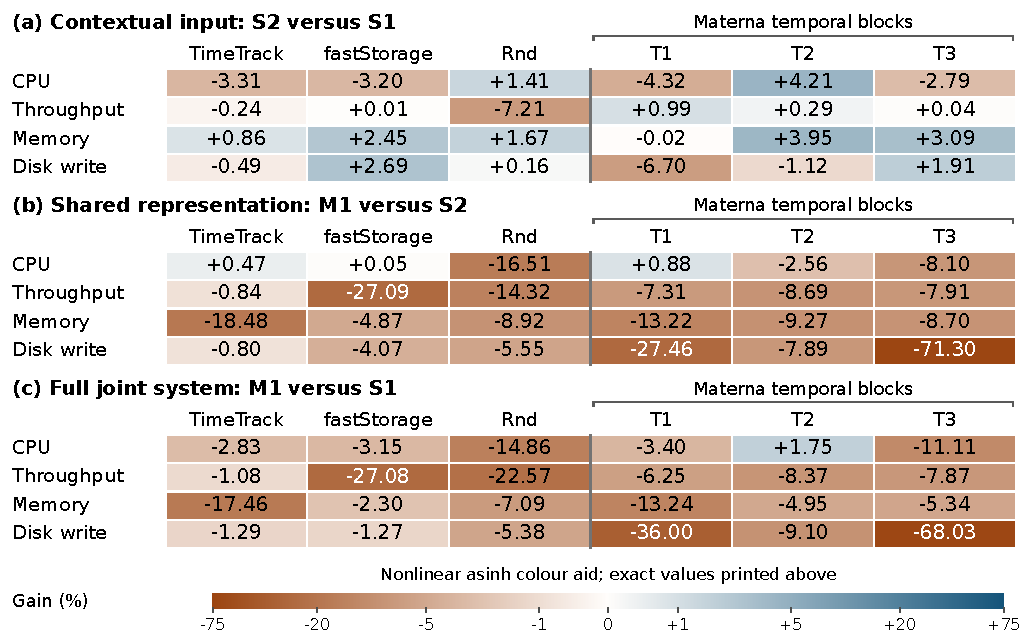
\includegraphics[width=\textwidth]{FigureS_G1.pdf}
\caption{Tier~1: prespecified resource-overall MacroMAE percentage gains for (a) S2 versus S1, (b) M1 versus S2
and (c) M1 versus S1 across the evaluated blocks. Positive values indicate lower MacroMAE for the candidate.
Colour uses a symmetric $\operatorname{asinh}$ mapping as a visual aid; no values are clipped and the printed
percentages are authoritative. Materna T1--T3 are dependent temporal blocks.}
\end{figure}

\begin{figure}[h]
\centering
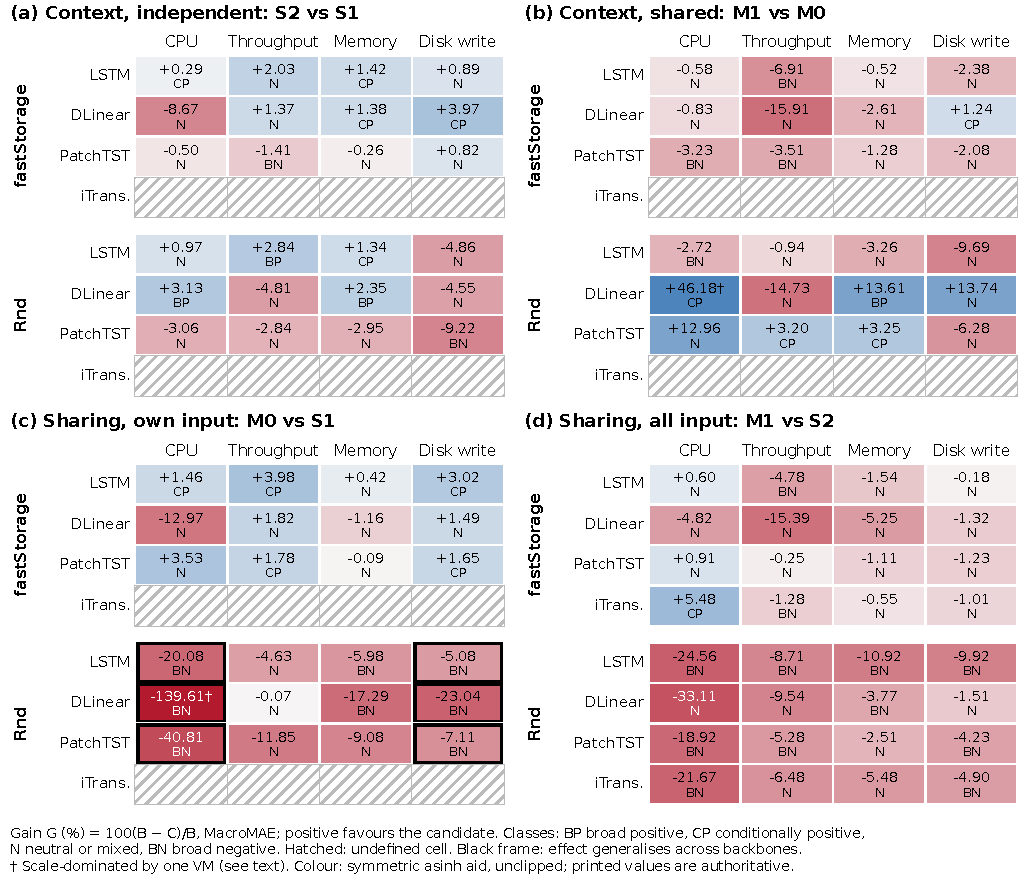
\includegraphics[width=\textwidth]{FigureS_G2.pdf}
\caption{Tier~2: prespecified resource-overall MacroMAE percentage gains on the 20-VM Bitbrains cohort for (a)
S2 versus S1, (b) M1 versus M0, (c) M0 versus S1 and (d) M1 versus S2, by backbone and block. Positive values
favour the candidate. Letters give the consistency class with VM thresholds rescaled to ten VMs. Hatched cells
are undefined by design. A black frame marks a cell where every defined backbone has a non-neutral class of the
same sign. $\dagger$: scale-dominated by one VM. Colour is a symmetric $\operatorname{asinh}$ visual aid without
clipping; printed values are authoritative.}
\end{figure}

\clearpage
\small
\begin{longtable}{@{}lllrrr@{}}
\caption{Post-hoc VM-cluster bootstrap intervals for the tier-2 matched-cell median MAE ratios (candidate/reference; 10{,}000 replicates resampling the ten VMs of each block with the frozen tier-2 draw matrices, seed 20261007; percentile 95\%). Point medians equal the frozen analysis output; win rates are the candidate's. An interval wholly above one means the ratio stays above one under resampling of the ten VMs; it indicates direction, not practical size, and percentile intervals from ten clusters may be too narrow. Computed after all results were known; descriptive.}\label{tab:supp-median-intervals}\\
\toprule
Contrast & Backbone & Block / resource & Ratio & 95\% interval & Win (\%) \\
\midrule
\endfirsthead
\toprule
Contrast & Backbone & Block / resource & Ratio & 95\% interval & Win (\%) \\
\midrule
\endhead
M1:S2 & LSTM & fastStorage CPU & 1.036 & [1.002, 1.094] & 35 \\
 &  & fastStorage Throughput & 1.053 & [1.013, 1.120] & 19 \\
 &  & fastStorage Memory & 1.001 & [0.997, 1.011] & 48 \\
 &  & fastStorage Disk write & 1.006 & [1.0002, 1.031] & 40 \\
 &  & Rnd CPU & 1.057 & [1.013, 1.097] & 28 \\
 &  & Rnd Throughput & 1.016 & [1.003, 1.042] & 23 \\
 &  & Rnd Memory & 1.015 & [1.005, 1.030] & 28 \\
 &  & Rnd Disk write & 1.039 & [1.007, 1.083] & 19 \\
\addlinespace
M1:S2 & DLinear & fastStorage CPU & 1.012 & [0.997, 1.051] & 40 \\
 &  & fastStorage Throughput & 1.006 & [1.001, 1.082] & 34 \\
 &  & fastStorage Memory & 1.003 & [0.9999, 1.014] & 37 \\
 &  & fastStorage Disk write & 1.00004 & [0.998, 1.014] & 50 \\
 &  & Rnd CPU & 1.011 & [1.003, 1.036] & 35 \\
 &  & Rnd Throughput & 1.004 & [0.9999, 1.016] & 42 \\
 &  & Rnd Memory & 1.005 & [1.003, 1.013] & 26 \\
 &  & Rnd Disk write & 1.007 & [1.003, 1.015] & 32 \\
\addlinespace
M1:S2 & PatchTST-style & fastStorage CPU & 1.006 & [0.980, 1.076] & 49 \\
 &  & fastStorage Throughput & 1.009 & [0.998, 1.080] & 41 \\
 &  & fastStorage Memory & 0.999 & [0.990, 1.013] & 50 \\
 &  & fastStorage Disk write & 1.004 & [0.9998, 1.034] & 41 \\
 &  & Rnd CPU & 1.037 & [1.016, 1.072] & 30 \\
 &  & Rnd Throughput & 1.003 & [0.997, 1.019] & 45 \\
 &  & Rnd Memory & 1.004 & [0.996, 1.022] & 43 \\
 &  & Rnd Disk write & 1.011 & [1.002, 1.058] & 34 \\
\addlinespace
M1:S2 & iTransformer-style & fastStorage CPU & 1.001 & [0.990, 1.019] & 49 \\
 &  & fastStorage Throughput & 1.029 & [1.010, 1.061] & 28 \\
 &  & fastStorage Memory & 0.9999 & [0.998, 1.003] & 51 \\
 &  & fastStorage Disk write & 1.001 & [0.995, 1.024] & 48 \\
 &  & Rnd CPU & 1.022 & [1.001, 1.054] & 35 \\
 &  & Rnd Throughput & 1.001 & [0.998, 1.010] & 48 \\
 &  & Rnd Memory & 1.006 & [0.9999, 1.024] & 39 \\
 &  & Rnd Disk write & 1.014 & [1.004, 1.043] & 32 \\
\addlinespace
M0:S1 & LSTM & fastStorage CPU & 0.999 & [0.978, 1.023] & 51 \\
 &  & fastStorage Throughput & 1.004 & [0.996, 1.035] & 43 \\
 &  & fastStorage Memory & 1.001 & [0.999, 1.006] & 43 \\
 &  & fastStorage Disk write & 1.001 & [0.999, 1.010] & 48 \\
 &  & Rnd CPU & 1.018 & [1.009, 1.036] & 33 \\
 &  & Rnd Throughput & 1.0003 & [0.998, 1.011] & 48 \\
 &  & Rnd Memory & 1.003 & [1.001, 1.021] & 33 \\
 &  & Rnd Disk write & 1.007 & [1.002, 1.029] & 33 \\
\addlinespace
M0:S1 & DLinear & fastStorage CPU & 1.017 & [0.983, 1.080] & 38 \\
 &  & fastStorage Throughput & 1.019 & [0.995, 1.058] & 42 \\
 &  & fastStorage Memory & 1.035 & [1.022, 1.065] & 18 \\
 &  & fastStorage Disk write & 1.004 & [0.991, 1.017] & 40 \\
 &  & Rnd CPU & 1.051 & [0.961, 1.247] & 34 \\
 &  & Rnd Throughput & 0.996 & [0.981, 1.009] & 61 \\
 &  & Rnd Memory & 1.059 & [1.022, 1.156] & 16 \\
 &  & Rnd Disk write & 1.023 & [1.008, 1.050] & 18 \\
\addlinespace
M0:S1 & PatchTST-style & fastStorage CPU & 1.011 & [0.994, 1.031] & 45 \\
 &  & fastStorage Throughput & 0.999 & [0.985, 1.017] & 53 \\
 &  & fastStorage Memory & 1.001 & [0.999, 1.008] & 47 \\
 &  & fastStorage Disk write & 0.9997 & [0.985, 1.004] & 51 \\
 &  & Rnd CPU & 1.027 & [1.008, 1.054] & 35 \\
 &  & Rnd Throughput & 1.007 & [1.001, 1.028] & 38 \\
 &  & Rnd Memory & 1.002 & [0.995, 1.015] & 45 \\
 &  & Rnd Disk write & 1.010 & [1.004, 1.035] & 35 \\
\addlinespace
S2:S1 & LSTM & fastStorage CPU & 0.985 & [0.941, 1.002] & 61 \\
 &  & fastStorage Throughput & 0.999 & [0.989, 1.005] & 52 \\
 &  & fastStorage Memory & 0.993 & [0.987, 1.004] & 62 \\
 &  & fastStorage Disk write & 1.003 & [0.997, 1.018] & 43 \\
 &  & Rnd CPU & 1.001 & [0.985, 1.038] & 50 \\
 &  & Rnd Throughput & 1.0001 & [0.992, 1.015] & 49 \\
 &  & Rnd Memory & 0.990 & [0.975, 1.007] & 61 \\
 &  & Rnd Disk write & 1.010 & [0.996, 1.047] & 38 \\
\addlinespace
S2:S1 & DLinear & fastStorage CPU & 1.012 & [0.972, 1.051] & 44 \\
 &  & fastStorage Throughput & 1.018 & [0.997, 1.084] & 42 \\
 &  & fastStorage Memory & 0.988 & [0.976, 1.003] & 65 \\
 &  & fastStorage Disk write & 0.981 & [0.951, 0.996] & 70 \\
 &  & Rnd CPU & 0.997 & [0.978, 1.005] & 52 \\
 &  & Rnd Throughput & 0.992 & [0.958, 1.007] & 58 \\
 &  & Rnd Memory & 0.990 & [0.969, 1.002] & 66 \\
 &  & Rnd Disk write & 0.997 & [0.991, 1.029] & 55 \\
\addlinespace
S2:S1 & PatchTST-style & fastStorage CPU & 1.035 & [1.002, 1.081] & 36 \\
 &  & fastStorage Throughput & 1.020 & [1.002, 1.058] & 34 \\
 &  & fastStorage Memory & 1.001 & [0.993, 1.014] & 48 \\
 &  & fastStorage Disk write & 1.010 & [0.999, 1.061] & 41 \\
 &  & Rnd CPU & 1.035 & [1.009, 1.061] & 36 \\
 &  & Rnd Throughput & 1.005 & [0.9996, 1.036] & 41 \\
 &  & Rnd Memory & 0.989 & [0.968, 1.014] & 59 \\
 &  & Rnd Disk write & 1.017 & [1.001, 1.060] & 35 \\
\addlinespace
M1:M0 & LSTM & fastStorage CPU & 1.025 & [1.001, 1.052] & 38 \\
 &  & fastStorage Throughput & 1.040 & [1.006, 1.158] & 26 \\
 &  & fastStorage Memory & 0.996 & [0.988, 1.011] & 55 \\
 &  & fastStorage Disk write & 1.009 & [0.999, 1.031] & 38 \\
 &  & Rnd CPU & 1.038 & [1.011, 1.086] & 35 \\
 &  & Rnd Throughput & 1.009 & [1.001, 1.043] & 34 \\
 &  & Rnd Memory & 0.995 & [0.988, 1.005] & 56 \\
 &  & Rnd Disk write & 1.034 & [0.999, 1.096] & 30 \\
\addlinespace
M1:M0 & DLinear & fastStorage CPU & 0.995 & [0.920, 1.102] & 52 \\
 &  & fastStorage Throughput & 1.020 & [0.991, 1.163] & 35 \\
 &  & fastStorage Memory & 0.960 & [0.924, 0.997] & 70 \\
 &  & fastStorage Disk write & 0.983 & [0.941, 1.010] & 63 \\
 &  & Rnd CPU & 0.928 & [0.802, 1.012] & 64 \\
 &  & Rnd Throughput & 1.006 & [0.976, 1.050] & 45 \\
 &  & Rnd Memory & 0.940 & [0.864, 0.971] & 83 \\
 &  & Rnd Disk write & 0.985 & [0.961, 1.015] & 62 \\
\addlinespace
M1:M0 & PatchTST-style & fastStorage CPU & 1.033 & [1.005, 1.077] & 36 \\
 &  & fastStorage Throughput & 1.059 & [1.012, 1.135] & 23 \\
 &  & fastStorage Memory & 0.995 & [0.990, 1.009] & 58 \\
 &  & fastStorage Disk write & 1.013 & [1.0005, 1.101] & 33 \\
 &  & Rnd CPU & 1.023 & [1.004, 1.052] & 34 \\
 &  & Rnd Throughput & 1.002 & [0.989, 1.024] & 47 \\
 &  & Rnd Memory & 0.994 & [0.981, 1.011] & 58 \\
 &  & Rnd Disk write & 1.038 & [1.0005, 1.107] & 31 \\
\bottomrule
\end{longtable}
\normalsize

\begin{table*}[t]
  \caption{Prespecified descriptive source summaries of primary overall MacroMAE
  gain (\%).}
  \label{tab:supp-synthesis}
  \centering
  \small
  \setlength{\tabcolsep}{3pt}
  \begin{tabular*}{\textwidth}{@{\extracolsep{\fill}}l*{9}{r}@{}}
    \toprule
    & \multicolumn{3}{c}{S2 versus S1}
      & \multicolumn{3}{c}{M1 versus S2}
      & \multicolumn{3}{c}{M1 versus S1} \\
    \cmidrule(lr){2-4}\cmidrule(lr){5-7}\cmidrule(l){8-10}
    Resource & TimeTrack & Bitbrains & Materna
      & TimeTrack & Bitbrains & Materna
      & TimeTrack & Bitbrains & Materna \\
    \midrule
    CPU & $-3.31$ & $-0.89$ & $-0.97$
      & $0.47$ & $-8.23$ & $-3.26$
      & $-2.83$ & $-9.01$ & $-4.25$ \\
    Throughput & $-0.24$ & $-3.60$ & $0.44$
      & $-0.84$ & $-20.71$ & $-7.97$
      & $-1.08$ & $-24.82$ & $-7.50$ \\
    Memory & $0.86$ & $2.06$ & $2.34$
      & $-18.48$ & $-6.89$ & $-10.40$
      & $-17.46$ & $-4.70$ & $-7.85$ \\
    Disk write & $-0.49$ & $1.42$ & $-1.97$
      & $-0.80$ & $-4.81$ & $-35.55$
      & $-1.29$ & $-3.33$ & $-37.71$ \\
    \midrule
    \multicolumn{10}{@{}l}{\emph{Tier~2 (Bitbrains, 20 VMs, every backbone
      defining the contrast): cells with negative gain / defined cells}} \\
    All resources & -- & 11/24 & -- & -- & 29/32 & -- & -- & -- & -- \\
    \bottomrule
  \end{tabular*}

  \vspace{2pt}
  \parbox{\textwidth}{\footnotesize
    Positive values indicate lower MacroMAE for the candidate formulation;
    negative values indicate higher MacroMAE. TimeTrack: development summary.
    Bitbrains: equal-environment synthesis of fastStorage and Rnd.
    Materna: equal-temporal-block synthesis of T1--T3, consecutive dependent
    temporal blocks rather than independent replications. Comparisons are
    descriptive, without cross-source aggregation. The tier-2 row counts
    backbone $\times$ resource $\times$ environment cells of tier~2
    (main-text Figure~3); it is not a gain,
    is not averaged with tier~1, and is not a replication of it. Tier~2 did
    not evaluate TimeTrack, Materna or M1 versus S1.}
\end{table*}

\clearpage
\section*{S-H Amendment A3: validation-gated consolidation and task grouping}
\label{sec:s-h}
Amendment A3 fits no model. It applies decision policies to the stored inner-validation and outer-test errors of
the tier-1 LSTM (six blocks) and the tier-2 backbones (20 Bitbrains VMs). It was frozen by the annotated tag
\texttt{fgcs-v04-a3-validation-gate} before any policy outcome was computed. The protocol is
\texttt{review\_revision/fgcs\_strengthening/validation\_gate\_amendment\_A3.md}; where the two differ, the
configuration \texttt{fgcs\_strengthening\_v04a3/configs/protocol\_v04a3.json} governs.

\emph{Unit and validation error.} A unit is a block $\times$ machine $\times$ fold $\times$ seed.
\begin{itemize}
  \item Tier~1 uses each fit's inner-validation MAE in training-scaled units at the selected context, averaged
    over leads.
  \item Tier~2 uses each inner fit's per-task scaled validation MSE at the epoch selected for the final refit.
\end{itemize}
A policy sees only its own unit's validation errors.

\emph{Policies.}
\begin{itemize}
  \item \emph{Fixed:} S1, S2, M0 (tier~2) and M1.
  \item \emph{G-ctx:} for each resource, S2 if it validates strictly better than S1.
  \item \emph{G-share($\tau$):} M1 if the mean over resources of the validation ratio M1/S2 is at most
    $1+\tau$, otherwise S2.
  \item \emph{G-full($\tau$):} the same, using the better-validating of M1 and M0 against the G-ctx baseline.
  \item \emph{G-group($\tau$), tier-2 LSTM:} the 15 partitions of the four resources into all-input models use
    S2 for singletons, the D-5 pair and triple models, and M1 for the full set. A partition is feasible if its
    mean validation ratio against S2 is at most $1+\tau$. The feasible partition with the fewest models is chosen;
    ties are broken by the lower ratio, then by a fixed order.
  \item \emph{Fallback, tier~2:} a target goes to persistence where persistence's validation MSE is strictly
    lower. The persistence MSE is computed on the same inner-validation windows, rebuilt and checked against their
    recorded hashes.
  \item \emph{Oracle, descriptive:} the candidate with the lowest outer score. It uses the outer test and is not a
    policy.
\end{itemize}
The tolerances are $\tau\in\{0,0.5,1,2\}\%$; $1\%$ is primary.

\emph{Outcomes.} Accuracy uses the main-text typical-cell statistics and the MacroMAE gains against S2, with
VM-cluster percentile intervals (seed 20261007, 10{,}000 replicates; tier~2 reuses its frozen draw matrices).
Savings retained is $R=(4-\text{models})/3$.

\emph{Decision rules.}
\begin{itemize}
  \item \emph{H-A3a:} ``keeps most savings at reduced cost'' if $R\ge0.5$ and the cost cells (median ratio above
    1.01) number at most half the M1:S2 count (22 in tier~1, 13 in tier~2); ``rarely consolidates'' if $R<0.25$.
  \item \emph{H-A3b:} ``detects'' if Spearman $\rho\ge0.3$ between the unit-level validation and outer M1/S2
    scores and its interval lies above zero.
  \item \emph{H-A3c:} ``grouping adds savings'' if G-group uses at least 0.25 fewer models per unit than G-share,
    with at most one more cost cell.
  \item \emph{Fallback:} ``restores positive skill'' if at least 8 of 16 CPU and throughput cells beat persistence.
\end{itemize}

\emph{Run and integrity.} The run took 147~s on one CPU thread from the tagged commit. Its output has SHA-256
\texttt{\seqsplit{33e11a858ea338b3c3ff25bec2f59527a3a2100a386658443def77956501cee0}}. Before the freeze, only the
input readers and the reproduction guards were run:
\begin{itemize}
  \item tier-1 seed means matched the published matched cells within a relative $3\times10^{-13}$;
  \item all 104 tier-2 fixed contrasts matched the frozen tier-2 output exactly;
  \item the persistence windows matched the recorded splits.
\end{itemize}
The verdicts were:
\begin{itemize}
  \item H-A3a: ``rarely consolidates'', in both tiers;
  \item H-A3b: ``detects'' in 12 of 14 frames;
  \item H-A3c: ``grouping adds savings'';
  \item fallback: ``does not restore positive skill''.
\end{itemize}
When a policy keeps most units on S2, the median matched-cell ratio is one by construction. The cost-cell counts
are then uninformative, and the savings and MacroMAE intervals carry the comparison.

% Generated by manuscript/fgcs/tools/a3_numbers.py; do not edit by hand.
\begin{table*}[t]\let\small\footnotesize
\centering
\caption{Amendment A3, consolidation policies per tier and backbone: savings retained $R=(4-\text{models})/3$ (\%) and typical-cell cost cells (policy:S2 median ratio above 1.01; of 4 cells per block) for G-share and G-full at each tolerance, and the reference M1 cost cells. G-ctx keeps four models and chooses S1 or S2 per resource.}
\label{tab:S-A3-gate}
\small
\begin{tabular}{@{}llcccccccccc@{}}
\toprule
 & & \multicolumn{4}{c}{G-share $R$ (cost) at $\tau$} & \multicolumn{4}{c}{G-full $R$ (cost) at $\tau$} & M1 & G-ctx \\
\cmidrule(lr){3-6}\cmidrule(lr){7-10}
Tier & Backbone, block & 0 & 0.5\% & 1\% & 2\% & 0 & 0.5\% & 1\% & 2\% & cost & cost \\
\midrule
1 & LSTM, TimeTrack & 3 (0) & 4 (0) & 5 (0) & 8 (0) & 1 (0) & 1 (0) & 2 (0) & 2 (0) & 2 & 0 \\
1 & LSTM, fastStorage & 5 (0) & 6 (0) & 8 (0) & 14 (0) & 3 (0) & 3 (0) & 4 (0) & 8 (0) & 4 & 0 \\
1 & LSTM, Rnd & 2 (0) & 3 (0) & 4 (0) & 8 (0) & 1 (0) & 2 (0) & 2 (0) & 4 (0) & 4 & 0 \\
1 & LSTM, Materna-T1 & 6 (0) & 8 (0) & 10 (0) & 17 (0) & 4 (0) & 5 (0) & 7 (0) & 11 (0) & 4 & 0 \\
1 & LSTM, Materna-T2 & 4 (0) & 6 (0) & 10 (0) & 18 (0) & 2 (0) & 3 (0) & 6 (0) & 13 (0) & 4 & 0 \\
1 & LSTM, Materna-T3 & 4 (0) & 5 (0) & 7 (0) & 14 (0) & 1 (0) & 2 (0) & 4 (0) & 8 (0) & 4 & 0 \\
2 & LSTM, fastStorage & 9 (0) & 12 (0) & 15 (0) & 29 (0) & 6 (0) & 11 (0) & 15 (0) & 31 (0) & 2 & 0 \\
2 & LSTM, Rnd & 2 (0) & 3 (0) & 6 (0) & 9 (0) & 5 (0) & 6 (0) & 9 (0) & 18 (0) & 4 & 0 \\
2 & DLinear, fastStorage & 16 (0) & 29 (0) & 35 (0) & 42 (0) & 15 (0) & 23 (0) & 33 (0) & 44 (0) & 1 & 0 \\
2 & DLinear, Rnd & 3 (0) & 17 (0) & 29 (0) & 41 (0) & 11 (0) & 24 (0) & 34 (0) & 44 (0) & 1 & 0 \\
2 & PatchTST-style, fastStorage & 8 (0) & 13 (0) & 21 (0) & 27 (0) & 2 (0) & 7 (0) & 18 (0) & 33 (0) & 0 & 0 \\
2 & PatchTST-style, Rnd & 4 (0) & 6 (0) & 11 (0) & 24 (0) & 8 (0) & 10 (0) & 13 (0) & 23 (0) & 2 & 0 \\
2 & iTransformer-style, fastStorage & 8 (0) & 15 (0) & 23 (0) & 30 (0) & 8 (0) & 15 (0) & 23 (0) & 30 (0) & 1 & -- \\
2 & iTransformer-style, Rnd & 8 (0) & 15 (0) & 21 (0) & 33 (0) & 8 (0) & 15 (0) & 21 (0) & 33 (0) & 2 & -- \\
\bottomrule
\end{tabular}
\end{table*}

\begin{table}[t]\let\small\footnotesize
\centering
\caption{Amendment A3, H-A3b: rank correlation between the unit-level validation score and the outer-test score of M1 against S2 (machine $\times$ fold $\times$ seed units), with VM-cluster interval, the share of units in which M1 was worse on validation and on the outer test, and the balanced accuracy of the validation sign.}
\label{tab:S-A3-detect}
\small
\setlength{\tabcolsep}{2.5pt}
\begin{tabular}{@{}lcccc@{}}
\toprule
Frame & $\rho$ [95\% interval] & Val./test worse & Bal. acc. & Verdict \\
\midrule
T1 TimeTrack & 0.30 [-0.08, 0.53] & 97/87\% & 0.48 & does not detect \\
T1 fastStorage & 0.52 [0.38, 0.63] & 95/82\% & 0.55 & detects \\
T1 Rnd & 0.55 [0.43, 0.64] & 98/94\% & 0.51 & detects \\
T1 Materna-T1 & 0.55 [0.36, 0.70] & 94/85\% & 0.56 & detects \\
T1 Materna-T2 & 0.66 [0.52, 0.76] & 96/86\% & 0.55 & detects \\
T1 Materna-T3 & 0.64 [0.49, 0.75] & 96/89\% & 0.56 & detects \\
T2 LSTM fastStorage & 0.31 [-0.00, 0.52] & 91/82\% & 0.54 & does not detect \\
T2 DLinear fastStorage & 0.64 [0.38, 0.77] & 84/74\% & 0.65 & detects \\
T2 PatchTST-style fastStorage & 0.34 [0.04, 0.54] & 92/66\% & 0.56 & detects \\
T2 iTransformer-style fastStorage & 0.30 [0.05, 0.47] & 92/67\% & 0.50 & detects \\
T2 LSTM Rnd & 0.53 [0.31, 0.67] & 98/90\% & 0.49 & detects \\
T2 DLinear Rnd & 0.46 [0.19, 0.64] & 97/77\% & 0.52 & detects \\
T2 PatchTST-style Rnd & 0.43 [0.02, 0.69] & 96/71\% & 0.50 & detects \\
T2 iTransformer-style Rnd & 0.34 [0.15, 0.51] & 92/77\% & 0.52 & detects \\
\bottomrule
\end{tabular}
\end{table}

\begin{table*}[t]\let\small\footnotesize
\centering
\caption{Amendment A3, tier-2 LSTM: G-group at $\tau=1\%$ and full sharing M1 against S2 per block and resource: matched-cell median MAE ratio [VM-cluster interval], win rate, MacroMAE gain (\%) [interval], and the share of units in which the resource stays in its own S2 model.}
\label{tab:S-A3-group}
\small
\begin{tabular}{@{}llccccc@{}}
\toprule
Block & Resource & G-group ratio & Win & G-group gain & Own model & M1 ratio / gain \\
\midrule
fastStorage & CPU & 1.000 [0.990, 1.003] & 0.46 & $+1.76$ [$-1.01$, $+2.69$] & 35\% & 1.036 / $+0.60$ \\
 & Throughput & 1.002 [1.000, 1.011] & 0.34 & $-3.05$ [$-8.34$, $-0.20$] & 28\% & 1.053 / $-4.78$ \\
 & Memory & 1.000 [0.995, 1.002] & 0.46 & $-0.83$ [$-2.73$, $+1.03$] & 21\% & 1.001 / $-1.54$ \\
 & Disk write & 0.999 [0.996, 1.001] & 0.53 & $+0.57$ [$-0.65$, $+2.06$] & 27\% & 1.006 / $-0.18$ \\
Rnd & CPU & 1.000 [1.000, 1.013] & 0.30 & $-0.36$ [$-1.80$, $+0.51$] & 37\% & 1.057 / $-24.56$ \\
 & Throughput & 1.000 [1.000, 1.004] & 0.26 & $-2.35$ [$-2.60$, $-0.32$] & 46\% & 1.016 / $-8.71$ \\
 & Memory & 1.000 [1.000, 1.002] & 0.34 & $-1.24$ [$-6.99$, $+0.71$] & 39\% & 1.015 / $-10.92$ \\
 & Disk write & 1.004 [1.002, 1.012] & 0.26 & $-5.74$ [$-18.10$, $-0.39$] & 27\% & 1.039 / $-9.92$ \\
\bottomrule
\end{tabular}
\end{table*}

\begin{table}[t]\let\small\footnotesize
\centering
\caption{Amendment A3, tier-2 LSTM: each of the 15 groupings applied to every unit (descriptive). Groups, cost cells and largest median ratio against S2 (of 8 cells), and the lowest MacroMAE gain (\%).}
\label{tab:S-A3-partitions}
\small
\setlength{\tabcolsep}{2.5pt}
\begin{tabular}{@{}lcccc@{}}
\toprule
Grouping & Groups & Cost & Max ratio & Lowest gain \\
\midrule
CTMD & 1 & 6 & 1.057 & $-24.56$ \\
C $\mid$ TMD & 2 & 2 & 1.039 & $-8.63$ \\
CD $\mid$ TM & 2 & 4 & 1.027 & $-8.69$ \\
CM $\mid$ TD & 2 & 2 & 1.017 & $-6.52$ \\
CMD $\mid$ T & 2 & 3 & 1.040 & $-10.82$ \\
CT $\mid$ MD & 2 & 4 & 1.049 & $-27.27$ \\
CTD $\mid$ M & 2 & 5 & 1.062 & $-27.69$ \\
CTM $\mid$ D & 2 & 5 & 1.045 & $-23.01$ \\
C $\mid$ T $\mid$ MD & 3 & 0 & 1.005 & $-9.63$ \\
C $\mid$ TD $\mid$ M & 3 & 2 & 1.017 & $-3.45$ \\
C $\mid$ TM $\mid$ D & 3 & 2 & 1.013 & $-8.69$ \\
CD $\mid$ T $\mid$ M & 3 & 2 & 1.027 & $-8.69$ \\
CM $\mid$ T $\mid$ D & 3 & 0 & 1.010 & $-6.52$ \\
CT $\mid$ M $\mid$ D & 3 & 4 & 1.049 & $-27.27$ \\
C $\mid$ T $\mid$ M $\mid$ D & 4 & 0 & 1.000 & $+0.00$ \\
\bottomrule
\end{tabular}

\vspace{2pt}\parbox{\columnwidth}{\footnotesize C, T, M, D: CPU, throughput, memory, disk write; letters in one group share a model.}
\end{table}

\begin{table}[t]\let\small\footnotesize
\centering
\caption{Amendment A3, persistence fallback (tier~2): persistence skill of S2 and of S2 with the validation-selected fallback for CPU and throughput, and the share of units sent to persistence.}
\label{tab:S-A3-fallback}
\small
\setlength{\tabcolsep}{2.5pt}
\begin{tabular}{@{}llccc@{}}
\toprule
Backbone, block & Resource & S2 & S2+fallback & Fallback units \\
\midrule
LSTM, fastStorage & CPU & $-0.701$ & $-0.602$ & 5\% \\
LSTM, fastStorage & Throughput & $-0.143$ & $+0.080$ & 19\% \\
LSTM, Rnd & CPU & $-0.299$ & $-0.269$ & 4\% \\
LSTM, Rnd & Throughput & $-0.044$ & $-0.018$ & 11\% \\
DLinear, fastStorage & CPU & $-0.163$ & $-0.098$ & 10\% \\
DLinear, fastStorage & Throughput & $-0.199$ & $+0.037$ & 25\% \\
DLinear, Rnd & CPU & $-0.090$ & $-0.079$ & 2\% \\
DLinear, Rnd & Throughput & $-0.066$ & $-0.020$ & 8\% \\
PatchTST-style, fastStorage & CPU & $-0.758$ & $-0.664$ & 6\% \\
PatchTST-style, fastStorage & Throughput & $-0.201$ & $+0.041$ & 20\% \\
PatchTST-style, Rnd & CPU & $-0.456$ & $-0.395$ & 4\% \\
PatchTST-style, Rnd & Throughput & $-0.110$ & $-0.091$ & 10\% \\
iTransformer-style, fastStorage & CPU & $-0.850$ & $-0.717$ & 9\% \\
iTransformer-style, fastStorage & Throughput & $-0.161$ & $-0.001$ & 18\% \\
iTransformer-style, Rnd & CPU & $-0.434$ & $-0.335$ & 4\% \\
iTransformer-style, Rnd & Throughput & $-0.136$ & $-0.061$ & 10\% \\
\bottomrule
\end{tabular}
\end{table}


\bibliographystyle{elsarticle-num-names}
\bibliography{references}
\end{document}
